\documentclass[twoside]{book}

% Packages required by doxygen
\usepackage{calc}
\usepackage{doxygen}
\usepackage{graphicx}
\usepackage[utf8]{inputenc}
\usepackage{makeidx}
\usepackage{multicol}
\usepackage{multirow}
\usepackage{textcomp}
\usepackage[table]{xcolor}

% Font selection
\usepackage[T1]{fontenc}
\usepackage{mathptmx}
\usepackage[scaled=.90]{helvet}
\usepackage{courier}
\usepackage{amssymb}
\usepackage{sectsty}
\renewcommand{\familydefault}{\sfdefault}
\allsectionsfont{%
  \fontseries{bc}\selectfont%
  \color{darkgray}%
}
\renewcommand{\DoxyLabelFont}{%
  \fontseries{bc}\selectfont%
  \color{darkgray}%
}

% Page & text layout
\usepackage{geometry}
\geometry{%
  a4paper,%
  top=2.5cm,%
  bottom=2.5cm,%
  left=2.5cm,%
  right=2.5cm%
}
\tolerance=750
\hfuzz=15pt
\hbadness=750
\setlength{\emergencystretch}{15pt}
\setlength{\parindent}{0cm}
\setlength{\parskip}{0.2cm}
\makeatletter
\renewcommand{\paragraph}{%
  \@startsection{paragraph}{4}{0ex}{-1.0ex}{1.0ex}{%
    \normalfont\normalsize\bfseries\SS@parafont%
  }%
}
\renewcommand{\subparagraph}{%
  \@startsection{subparagraph}{5}{0ex}{-1.0ex}{1.0ex}{%
    \normalfont\normalsize\bfseries\SS@subparafont%
  }%
}
\makeatother

% Headers & footers
\usepackage{fancyhdr}
\pagestyle{fancyplain}
\fancyhead[LE]{\fancyplain{}{\bfseries\thepage}}
\fancyhead[CE]{\fancyplain{}{}}
\fancyhead[RE]{\fancyplain{}{\bfseries\leftmark}}
\fancyhead[LO]{\fancyplain{}{\bfseries\rightmark}}
\fancyhead[CO]{\fancyplain{}{}}
\fancyhead[RO]{\fancyplain{}{\bfseries\thepage}}
\fancyfoot[LE]{\fancyplain{}{}}
\fancyfoot[CE]{\fancyplain{}{}}
\fancyfoot[RE]{\fancyplain{}{\bfseries\scriptsize Generated on Sat Mar 14 2015 23\-:13\-:50 for Robot Simulation by Doxygen }}
\fancyfoot[LO]{\fancyplain{}{\bfseries\scriptsize Generated on Sat Mar 14 2015 23\-:13\-:50 for Robot Simulation by Doxygen }}
\fancyfoot[CO]{\fancyplain{}{}}
\fancyfoot[RO]{\fancyplain{}{}}
\renewcommand{\footrulewidth}{0.4pt}
\renewcommand{\chaptermark}[1]{%
  \markboth{#1}{}%
}
\renewcommand{\sectionmark}[1]{%
  \markright{\thesection\ #1}%
}

% Indices & bibliography
\usepackage{natbib}
\usepackage[titles]{tocloft}
\setcounter{tocdepth}{3}
\setcounter{secnumdepth}{5}
\makeindex

% Hyperlinks (required, but should be loaded last)
\usepackage{ifpdf}
\ifpdf
  \usepackage[pdftex,pagebackref=true]{hyperref}
\else
  \usepackage[ps2pdf,pagebackref=true]{hyperref}
\fi
\hypersetup{%
  colorlinks=true,%
  linkcolor=blue,%
  citecolor=blue,%
  unicode%
}

% Custom commands
\newcommand{\clearemptydoublepage}{%
  \newpage{\pagestyle{empty}\cleardoublepage}%
}


%===== C O N T E N T S =====

\begin{document}

% Titlepage & ToC
\hypersetup{pageanchor=false}
\pagenumbering{roman}
\begin{titlepage}
\vspace*{7cm}
\begin{center}%
{\Large Robot Simulation }\\
\vspace*{1cm}
{\large Generated by Doxygen 1.8.6}\\
\vspace*{0.5cm}
{\small Sat Mar 14 2015 23:13:50}\\
\end{center}
\end{titlepage}
\clearemptydoublepage
\tableofcontents
\clearemptydoublepage
\pagenumbering{arabic}
\hypersetup{pageanchor=true}

%--- Begin generated contents ---
\chapter{Hierarchical Index}
\section{Class Hierarchy}
This inheritance list is sorted roughly, but not completely, alphabetically\-:\begin{DoxyCompactList}
\item \contentsline{section}{Base\-Gfx\-App}{\pageref{classBaseGfxApp}}{}
\begin{DoxyCompactList}
\item \contentsline{section}{Simulation}{\pageref{classSimulation}}{}
\end{DoxyCompactList}
\item \contentsline{section}{Environment\-Class}{\pageref{classEnvironmentClass}}{}
\item \contentsline{section}{Navigate}{\pageref{structNavigate}}{}
\item \contentsline{section}{Object}{\pageref{classObject}}{}
\item Test\-Suite\begin{DoxyCompactList}
\item \contentsline{section}{Environment\-Class\-Test}{\pageref{classEnvironmentClassTest}}{}
\item \contentsline{section}{Object\-Tests}{\pageref{classObjectTests}}{}
\end{DoxyCompactList}
\end{DoxyCompactList}

\chapter{Class Index}
\section{Class List}
Here are the classes, structs, unions and interfaces with brief descriptions\-:\begin{DoxyCompactList}
\item\contentsline{section}{\hyperlink{classBaseGfxApp}{Base\-Gfx\-App} }{\pageref{classBaseGfxApp}}{}
\item\contentsline{section}{\hyperlink{classEnvironmentClass}{Environment\-Class} }{\pageref{classEnvironmentClass}}{}
\item\contentsline{section}{\hyperlink{classLight}{Light} \\*A light class contains attributes and behaviors }{\pageref{classLight}}{}
\item\contentsline{section}{\hyperlink{classRobotClass}{Robot\-Class} \\*A robot class contains attributes and hehaviors }{\pageref{classRobotClass}}{}
\item\contentsline{section}{\hyperlink{classSensor}{Sensor} }{\pageref{classSensor}}{}
\item\contentsline{section}{\hyperlink{classShape}{Shape} \\*Super Class of \hyperlink{classRobotClass}{Robot\-Class}, Target and Obstacle, contains position x, y, width and length }{\pageref{classShape}}{}
\item\contentsline{section}{\hyperlink{classSimulation}{Simulation} }{\pageref{classSimulation}}{}
\item\contentsline{section}{\hyperlink{classWheel}{Wheel} }{\pageref{classWheel}}{}
\end{DoxyCompactList}

\chapter{File Index}
\section{File List}
Here is a list of all files with brief descriptions\-:\begin{DoxyCompactList}
\item\contentsline{section}{\hyperlink{BaseGfxApp_8cpp}{Base\-Gfx\-App.\-cpp} }{\pageref{BaseGfxApp_8cpp}}{}
\item\contentsline{section}{\hyperlink{BaseGfxApp_8h}{Base\-Gfx\-App.\-h} \\*The basic application class for C\-Sci-\/3081 project. Uses G\-L\-U\-T and G\-L\-U\-I and wraps them in a nice C++ interface }{\pageref{BaseGfxApp_8h}}{}
\item\contentsline{section}{\hyperlink{EnvironmentClass_8cpp}{Environment\-Class.\-cpp} }{\pageref{EnvironmentClass_8cpp}}{}
\item\contentsline{section}{\hyperlink{EnvironmentClass_8h}{Environment\-Class.\-h} \\*Main application class for the Environment Class }{\pageref{EnvironmentClass_8h}}{}
\item\contentsline{section}{\hyperlink{EnvironmentClassTest_8h}{Environment\-Class\-Test.\-h} \\*The Tests for environment functions }{\pageref{EnvironmentClassTest_8h}}{}
\item\contentsline{section}{\hyperlink{main_8cpp}{main.\-cpp} \\*Main function }{\pageref{main_8cpp}}{}
\item\contentsline{section}{\hyperlink{Object_8cpp}{Object.\-cpp} \\*The representation of \hyperlink{classObject}{Object} within the simulation }{\pageref{Object_8cpp}}{}
\item\contentsline{section}{\hyperlink{Object_8h}{Object.\-h} \\*The \hyperlink{classObject}{Object} Class }{\pageref{Object_8h}}{}
\item\contentsline{section}{\hyperlink{ObjectTests_8h}{Object\-Tests.\-h} }{\pageref{ObjectTests_8h}}{}
\item\contentsline{section}{\hyperlink{Simulation_8cpp}{Simulation.\-cpp} }{\pageref{Simulation_8cpp}}{}
\item\contentsline{section}{\hyperlink{Simulation_8h}{Simulation.\-h} \\*Main application class for the robot simulation }{\pageref{Simulation_8h}}{}
\end{DoxyCompactList}

\chapter{Class Documentation}
\hypertarget{classBaseGfxApp}{\section{Base\-Gfx\-App Class Reference}
\label{classBaseGfxApp}\index{Base\-Gfx\-App@{Base\-Gfx\-App}}
}


{\ttfamily \#include $<$Base\-Gfx\-App.\-h$>$}

Inheritance diagram for Base\-Gfx\-App\-:\begin{figure}[H]
\begin{center}
\leavevmode
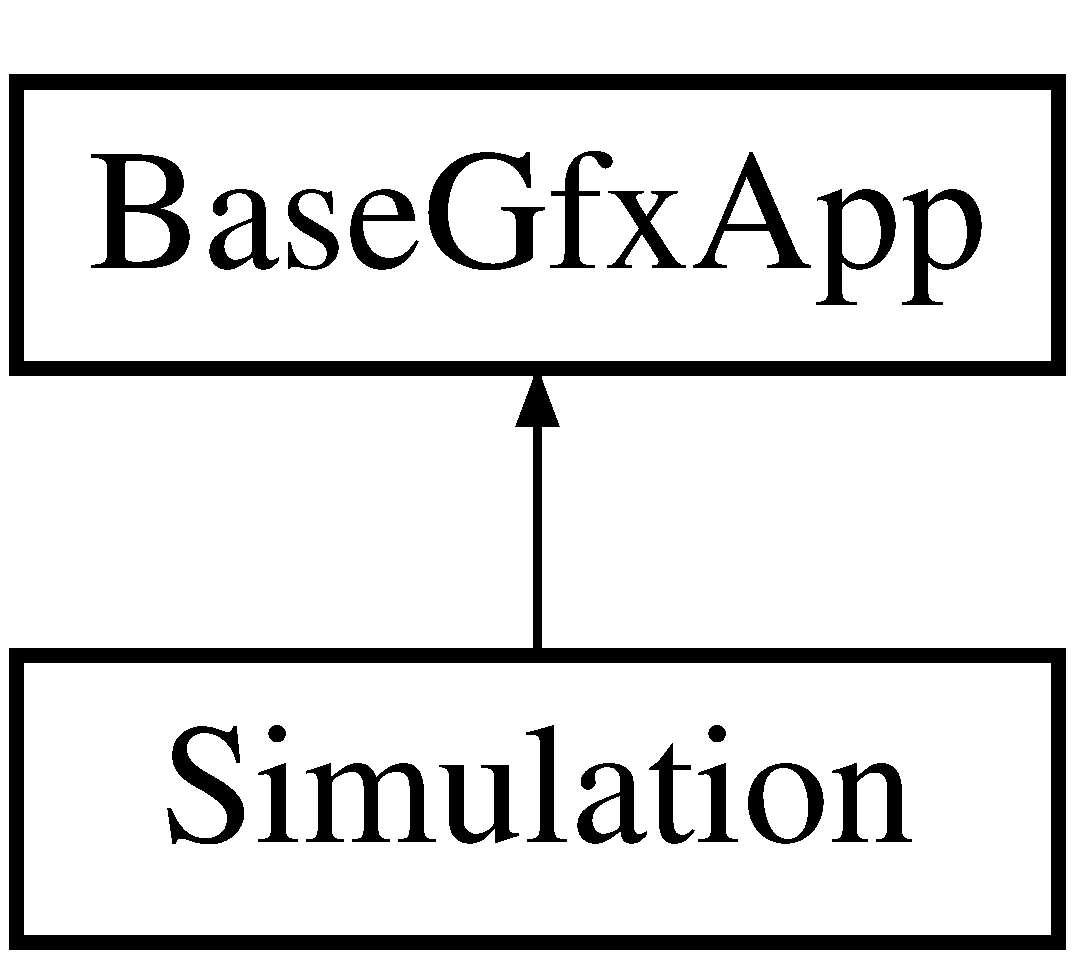
\includegraphics[height=2.000000cm]{classBaseGfxApp}
\end{center}
\end{figure}
\subsection*{Public Member Functions}
\begin{DoxyCompactItemize}
\item 
\hyperlink{classBaseGfxApp_a534a4b5293a35947fdae3805a103541d}{Base\-Gfx\-App} (int argc, char $\ast$argv\mbox{[}$\,$\mbox{]}, int \hyperlink{classBaseGfxApp_ace089a1a94fb6bb0bc17e1b7fa48e05d}{width}, int \hyperlink{classBaseGfxApp_aa253dbe16a20c40e0a1bf8ff942ceea3}{height}, int x, int y, int glut\-Flags, bool create\-G\-L\-U\-I\-Win, int glui\-Win\-X, int glui\-Win\-Y)
\item 
virtual \hyperlink{classBaseGfxApp_aceb6194bd818c0ffa980a6990fd03027}{$\sim$\-Base\-Gfx\-App} ()
\item 
void \hyperlink{classBaseGfxApp_a4b3b1a475b7f2babaf1b477c34b15fb1}{set\-Caption} (const std\-::string \&caption)
\item 
void \hyperlink{classBaseGfxApp_acda031916c00d56c2dc901e2653e3083}{run\-Main\-Loop} ()
\item 
virtual void \hyperlink{classBaseGfxApp_ac8de2d5a955582547af5619b771b4d6d}{display} ()
\item 
virtual void \hyperlink{classBaseGfxApp_a0956b82d7fa58b623c498aea7073dbba}{mouse\-Moved} (int x, int y)
\item 
virtual void \hyperlink{classBaseGfxApp_abb23f716dd6612b3a72938e41525d338}{mouse\-Dragged} (int x, int y)
\item 
virtual void \hyperlink{classBaseGfxApp_aaaccf5a5e923a9465441a5ee712424a8}{left\-Mouse\-Down} (int x, int y)
\item 
virtual void \hyperlink{classBaseGfxApp_a0a2961a932b02b2f9d7d0bb408f6fb51}{left\-Mouse\-Up} (int x, int y)
\item 
virtual void \hyperlink{classBaseGfxApp_afa87e6a71220945e41f0424e540125d9}{right\-Mouse\-Down} (int x, int y)
\item 
virtual void \hyperlink{classBaseGfxApp_a812643d563522a993457dd565c33f8f6}{right\-Mouse\-Up} (int x, int y)
\item 
virtual void \hyperlink{classBaseGfxApp_a2c98cae9bb5ad1fb1832a6d4812670f8}{middle\-Mouse\-Down} (int x, int y)
\item 
virtual void \hyperlink{classBaseGfxApp_a00fc05e8d9629b72302b5adf014bdb0c}{middle\-Mouse\-Up} (int x, int y)
\item 
virtual void \hyperlink{classBaseGfxApp_a6d91e0cb7a3d48cad33956efe7eb36ca}{keyboard} (unsigned char c, int x, int y)
\item 
virtual void \hyperlink{classBaseGfxApp_a345566e62c9e4ec3705ec4d1c4c75f1f}{keyboard\-Special} (int key, int x, int y)
\item 
virtual void \hyperlink{classBaseGfxApp_acc4a40ce11edd6b6660a19cb4802a2bf}{keyboard\-Up} (unsigned char c, int x, int y)
\item 
virtual void \hyperlink{classBaseGfxApp_afd14b435ff93b1e7f461cb8bd1a6fd59}{keyboard\-Special\-Up} (int key, int x, int y)
\item 
virtual void \hyperlink{classBaseGfxApp_a5d8d5d778a8aecd7f5f8e9c87f4c3d20}{reshape} (int \hyperlink{classBaseGfxApp_ace089a1a94fb6bb0bc17e1b7fa48e05d}{width}, int \hyperlink{classBaseGfxApp_aa253dbe16a20c40e0a1bf8ff942ceea3}{height})
\item 
virtual void \hyperlink{classBaseGfxApp_a2978a7c358794c67df73b66776b2cef3}{glui\-Control} (int control\-I\-D)
\item 
int \hyperlink{classBaseGfxApp_ace089a1a94fb6bb0bc17e1b7fa48e05d}{width} () const 
\item 
int \hyperlink{classBaseGfxApp_aa253dbe16a20c40e0a1bf8ff942ceea3}{height} () const 
\item 
int \hyperlink{classBaseGfxApp_ae9779f948eff6f45beec08091e98a803}{handle} ()
\item 
G\-L\-U\-I $\ast$ \hyperlink{classBaseGfxApp_ac721a0fedce80308c5c0e5695016e95d}{glui} ()
\end{DoxyCompactItemize}
\subsection*{Static Protected Member Functions}
\begin{DoxyCompactItemize}
\item 
static void \hyperlink{classBaseGfxApp_a5fe6a77d37044cbe28647ed3391bbb7a}{s\-\_\-reshape} (int \hyperlink{classBaseGfxApp_ace089a1a94fb6bb0bc17e1b7fa48e05d}{width}, int \hyperlink{classBaseGfxApp_aa253dbe16a20c40e0a1bf8ff942ceea3}{height})
\item 
static void \hyperlink{classBaseGfxApp_a52edb2569227319feb68779844e7d857}{s\-\_\-keyboard} (unsigned char c, int x, int y)
\item 
static void \hyperlink{classBaseGfxApp_a1e8d90a4faab60300ddf2a4ea9b83115}{s\-\_\-keyboardspecial} (int key, int x, int y)
\item 
static void \hyperlink{classBaseGfxApp_aa1ca205af9d6cee33949f2e6adf4c923}{s\-\_\-keyboardup} (unsigned char c, int x, int y)
\item 
static void \hyperlink{classBaseGfxApp_a0e4dfe006f3cc9126c1cc8ad32784f75}{s\-\_\-keyboardspecialup} (int key, int x, int y)
\item 
static void \hyperlink{classBaseGfxApp_a5e640f2394f7e038d0dd2b469d5c2e24}{s\-\_\-mousemotion} (int x, int y)
\item 
static void \hyperlink{classBaseGfxApp_a22dd953bfb75add9fd0f8f2f8be535c5}{s\-\_\-mousebtn} (int b, int s, int x, int y)
\item 
static void \hyperlink{classBaseGfxApp_a58415c6151a2a80e1fe2eaa9919a4dab}{s\-\_\-draw} ()
\item 
static void \hyperlink{classBaseGfxApp_ad4a963321f1147d68369225ab0c7f32f}{s\-\_\-gluicallback} (int control\-I\-D)
\end{DoxyCompactItemize}
\subsection*{Protected Attributes}
\begin{DoxyCompactItemize}
\item 
int \hyperlink{classBaseGfxApp_ad8697d6fdd10e6f336c3a662016b4fa7}{m\-\_\-glut\-Window\-Handle}
\item 
G\-L\-U\-I $\ast$ \hyperlink{classBaseGfxApp_a6eb1673b80283727221da2242211af1d}{m\-\_\-glui}
\item 
bool \hyperlink{classBaseGfxApp_a2e70a389224f8affe7c137f7e20dc8c1}{m\-\_\-drag}
\item 
int \hyperlink{classBaseGfxApp_a7e5ef1c8f25fe081b4a1fd4ce6a96e07}{m\-\_\-width}
\item 
int \hyperlink{classBaseGfxApp_ac078e4fc20b5c2fe0c744966b850b412}{m\-\_\-height}
\end{DoxyCompactItemize}
\subsection*{Static Protected Attributes}
\begin{DoxyCompactItemize}
\item 
static \hyperlink{classBaseGfxApp}{Base\-Gfx\-App} $\ast$ \hyperlink{classBaseGfxApp_a65ba89b98af31e2649a0546631931000}{s\-\_\-current\-App} = N\-U\-L\-L
\item 
static bool \hyperlink{classBaseGfxApp_afa4690383ea27713016ef75b9fb1e42f}{s\-\_\-glut\-Initialized} = false
\end{DoxyCompactItemize}


\subsection{Constructor \& Destructor Documentation}
\hypertarget{classBaseGfxApp_a534a4b5293a35947fdae3805a103541d}{\index{Base\-Gfx\-App@{Base\-Gfx\-App}!Base\-Gfx\-App@{Base\-Gfx\-App}}
\index{Base\-Gfx\-App@{Base\-Gfx\-App}!BaseGfxApp@{Base\-Gfx\-App}}
\subsubsection[{Base\-Gfx\-App}]{\setlength{\rightskip}{0pt plus 5cm}Base\-Gfx\-App\-::\-Base\-Gfx\-App (
\begin{DoxyParamCaption}
\item[{int}]{argc, }
\item[{char $\ast$}]{argv\mbox{[}$\,$\mbox{]}, }
\item[{int}]{width, }
\item[{int}]{height, }
\item[{int}]{x, }
\item[{int}]{y, }
\item[{int}]{glut\-Flags, }
\item[{bool}]{create\-G\-L\-U\-I\-Win, }
\item[{int}]{glui\-Win\-X, }
\item[{int}]{glui\-Win\-Y}
\end{DoxyParamCaption}
)}}\label{classBaseGfxApp_a534a4b5293a35947fdae3805a103541d}
\hypertarget{classBaseGfxApp_aceb6194bd818c0ffa980a6990fd03027}{\index{Base\-Gfx\-App@{Base\-Gfx\-App}!$\sim$\-Base\-Gfx\-App@{$\sim$\-Base\-Gfx\-App}}
\index{$\sim$\-Base\-Gfx\-App@{$\sim$\-Base\-Gfx\-App}!BaseGfxApp@{Base\-Gfx\-App}}
\subsubsection[{$\sim$\-Base\-Gfx\-App}]{\setlength{\rightskip}{0pt plus 5cm}Base\-Gfx\-App\-::$\sim$\-Base\-Gfx\-App (
\begin{DoxyParamCaption}
{}
\end{DoxyParamCaption}
)\hspace{0.3cm}{\ttfamily [virtual]}}}\label{classBaseGfxApp_aceb6194bd818c0ffa980a6990fd03027}


\subsection{Member Function Documentation}
\hypertarget{classBaseGfxApp_ac8de2d5a955582547af5619b771b4d6d}{\index{Base\-Gfx\-App@{Base\-Gfx\-App}!display@{display}}
\index{display@{display}!BaseGfxApp@{Base\-Gfx\-App}}
\subsubsection[{display}]{\setlength{\rightskip}{0pt plus 5cm}virtual void Base\-Gfx\-App\-::display (
\begin{DoxyParamCaption}
{}
\end{DoxyParamCaption}
)\hspace{0.3cm}{\ttfamily [inline]}, {\ttfamily [virtual]}}}\label{classBaseGfxApp_ac8de2d5a955582547af5619b771b4d6d}


Reimplemented in \hyperlink{classSimulation_a449dcb7d97dfba99efe770de2f399c31}{Simulation}.

\hypertarget{classBaseGfxApp_ac721a0fedce80308c5c0e5695016e95d}{\index{Base\-Gfx\-App@{Base\-Gfx\-App}!glui@{glui}}
\index{glui@{glui}!BaseGfxApp@{Base\-Gfx\-App}}
\subsubsection[{glui}]{\setlength{\rightskip}{0pt plus 5cm}G\-L\-U\-I$\ast$ Base\-Gfx\-App\-::glui (
\begin{DoxyParamCaption}
{}
\end{DoxyParamCaption}
)\hspace{0.3cm}{\ttfamily [inline]}}}\label{classBaseGfxApp_ac721a0fedce80308c5c0e5695016e95d}
\hypertarget{classBaseGfxApp_a2978a7c358794c67df73b66776b2cef3}{\index{Base\-Gfx\-App@{Base\-Gfx\-App}!glui\-Control@{glui\-Control}}
\index{glui\-Control@{glui\-Control}!BaseGfxApp@{Base\-Gfx\-App}}
\subsubsection[{glui\-Control}]{\setlength{\rightskip}{0pt plus 5cm}virtual void Base\-Gfx\-App\-::glui\-Control (
\begin{DoxyParamCaption}
\item[{int}]{control\-I\-D}
\end{DoxyParamCaption}
)\hspace{0.3cm}{\ttfamily [inline]}, {\ttfamily [virtual]}}}\label{classBaseGfxApp_a2978a7c358794c67df73b66776b2cef3}


Reimplemented in \hyperlink{classSimulation_a1607cd18e552ab9f4a6f57d362f7121a}{Simulation}.

\hypertarget{classBaseGfxApp_ae9779f948eff6f45beec08091e98a803}{\index{Base\-Gfx\-App@{Base\-Gfx\-App}!handle@{handle}}
\index{handle@{handle}!BaseGfxApp@{Base\-Gfx\-App}}
\subsubsection[{handle}]{\setlength{\rightskip}{0pt plus 5cm}int Base\-Gfx\-App\-::handle (
\begin{DoxyParamCaption}
{}
\end{DoxyParamCaption}
)\hspace{0.3cm}{\ttfamily [inline]}}}\label{classBaseGfxApp_ae9779f948eff6f45beec08091e98a803}
\hypertarget{classBaseGfxApp_aa253dbe16a20c40e0a1bf8ff942ceea3}{\index{Base\-Gfx\-App@{Base\-Gfx\-App}!height@{height}}
\index{height@{height}!BaseGfxApp@{Base\-Gfx\-App}}
\subsubsection[{height}]{\setlength{\rightskip}{0pt plus 5cm}int Base\-Gfx\-App\-::height (
\begin{DoxyParamCaption}
{}
\end{DoxyParamCaption}
) const}}\label{classBaseGfxApp_aa253dbe16a20c40e0a1bf8ff942ceea3}
\hypertarget{classBaseGfxApp_a6d91e0cb7a3d48cad33956efe7eb36ca}{\index{Base\-Gfx\-App@{Base\-Gfx\-App}!keyboard@{keyboard}}
\index{keyboard@{keyboard}!BaseGfxApp@{Base\-Gfx\-App}}
\subsubsection[{keyboard}]{\setlength{\rightskip}{0pt plus 5cm}virtual void Base\-Gfx\-App\-::keyboard (
\begin{DoxyParamCaption}
\item[{unsigned char}]{c, }
\item[{int}]{x, }
\item[{int}]{y}
\end{DoxyParamCaption}
)\hspace{0.3cm}{\ttfamily [inline]}, {\ttfamily [virtual]}}}\label{classBaseGfxApp_a6d91e0cb7a3d48cad33956efe7eb36ca}
\hypertarget{classBaseGfxApp_a345566e62c9e4ec3705ec4d1c4c75f1f}{\index{Base\-Gfx\-App@{Base\-Gfx\-App}!keyboard\-Special@{keyboard\-Special}}
\index{keyboard\-Special@{keyboard\-Special}!BaseGfxApp@{Base\-Gfx\-App}}
\subsubsection[{keyboard\-Special}]{\setlength{\rightskip}{0pt plus 5cm}virtual void Base\-Gfx\-App\-::keyboard\-Special (
\begin{DoxyParamCaption}
\item[{int}]{key, }
\item[{int}]{x, }
\item[{int}]{y}
\end{DoxyParamCaption}
)\hspace{0.3cm}{\ttfamily [inline]}, {\ttfamily [virtual]}}}\label{classBaseGfxApp_a345566e62c9e4ec3705ec4d1c4c75f1f}
\hypertarget{classBaseGfxApp_afd14b435ff93b1e7f461cb8bd1a6fd59}{\index{Base\-Gfx\-App@{Base\-Gfx\-App}!keyboard\-Special\-Up@{keyboard\-Special\-Up}}
\index{keyboard\-Special\-Up@{keyboard\-Special\-Up}!BaseGfxApp@{Base\-Gfx\-App}}
\subsubsection[{keyboard\-Special\-Up}]{\setlength{\rightskip}{0pt plus 5cm}virtual void Base\-Gfx\-App\-::keyboard\-Special\-Up (
\begin{DoxyParamCaption}
\item[{int}]{key, }
\item[{int}]{x, }
\item[{int}]{y}
\end{DoxyParamCaption}
)\hspace{0.3cm}{\ttfamily [inline]}, {\ttfamily [virtual]}}}\label{classBaseGfxApp_afd14b435ff93b1e7f461cb8bd1a6fd59}
\hypertarget{classBaseGfxApp_acc4a40ce11edd6b6660a19cb4802a2bf}{\index{Base\-Gfx\-App@{Base\-Gfx\-App}!keyboard\-Up@{keyboard\-Up}}
\index{keyboard\-Up@{keyboard\-Up}!BaseGfxApp@{Base\-Gfx\-App}}
\subsubsection[{keyboard\-Up}]{\setlength{\rightskip}{0pt plus 5cm}virtual void Base\-Gfx\-App\-::keyboard\-Up (
\begin{DoxyParamCaption}
\item[{unsigned char}]{c, }
\item[{int}]{x, }
\item[{int}]{y}
\end{DoxyParamCaption}
)\hspace{0.3cm}{\ttfamily [inline]}, {\ttfamily [virtual]}}}\label{classBaseGfxApp_acc4a40ce11edd6b6660a19cb4802a2bf}
\hypertarget{classBaseGfxApp_aaaccf5a5e923a9465441a5ee712424a8}{\index{Base\-Gfx\-App@{Base\-Gfx\-App}!left\-Mouse\-Down@{left\-Mouse\-Down}}
\index{left\-Mouse\-Down@{left\-Mouse\-Down}!BaseGfxApp@{Base\-Gfx\-App}}
\subsubsection[{left\-Mouse\-Down}]{\setlength{\rightskip}{0pt plus 5cm}virtual void Base\-Gfx\-App\-::left\-Mouse\-Down (
\begin{DoxyParamCaption}
\item[{int}]{x, }
\item[{int}]{y}
\end{DoxyParamCaption}
)\hspace{0.3cm}{\ttfamily [inline]}, {\ttfamily [virtual]}}}\label{classBaseGfxApp_aaaccf5a5e923a9465441a5ee712424a8}


Reimplemented in \hyperlink{classSimulation_a786d1ba31d29937f0ac6f3ea88f8a607}{Simulation}.

\hypertarget{classBaseGfxApp_a0a2961a932b02b2f9d7d0bb408f6fb51}{\index{Base\-Gfx\-App@{Base\-Gfx\-App}!left\-Mouse\-Up@{left\-Mouse\-Up}}
\index{left\-Mouse\-Up@{left\-Mouse\-Up}!BaseGfxApp@{Base\-Gfx\-App}}
\subsubsection[{left\-Mouse\-Up}]{\setlength{\rightskip}{0pt plus 5cm}virtual void Base\-Gfx\-App\-::left\-Mouse\-Up (
\begin{DoxyParamCaption}
\item[{int}]{x, }
\item[{int}]{y}
\end{DoxyParamCaption}
)\hspace{0.3cm}{\ttfamily [inline]}, {\ttfamily [virtual]}}}\label{classBaseGfxApp_a0a2961a932b02b2f9d7d0bb408f6fb51}


Reimplemented in \hyperlink{classSimulation_a62ef254d85017074cd521a5787b5a234}{Simulation}.

\hypertarget{classBaseGfxApp_a2c98cae9bb5ad1fb1832a6d4812670f8}{\index{Base\-Gfx\-App@{Base\-Gfx\-App}!middle\-Mouse\-Down@{middle\-Mouse\-Down}}
\index{middle\-Mouse\-Down@{middle\-Mouse\-Down}!BaseGfxApp@{Base\-Gfx\-App}}
\subsubsection[{middle\-Mouse\-Down}]{\setlength{\rightskip}{0pt plus 5cm}virtual void Base\-Gfx\-App\-::middle\-Mouse\-Down (
\begin{DoxyParamCaption}
\item[{int}]{x, }
\item[{int}]{y}
\end{DoxyParamCaption}
)\hspace{0.3cm}{\ttfamily [inline]}, {\ttfamily [virtual]}}}\label{classBaseGfxApp_a2c98cae9bb5ad1fb1832a6d4812670f8}
\hypertarget{classBaseGfxApp_a00fc05e8d9629b72302b5adf014bdb0c}{\index{Base\-Gfx\-App@{Base\-Gfx\-App}!middle\-Mouse\-Up@{middle\-Mouse\-Up}}
\index{middle\-Mouse\-Up@{middle\-Mouse\-Up}!BaseGfxApp@{Base\-Gfx\-App}}
\subsubsection[{middle\-Mouse\-Up}]{\setlength{\rightskip}{0pt plus 5cm}virtual void Base\-Gfx\-App\-::middle\-Mouse\-Up (
\begin{DoxyParamCaption}
\item[{int}]{x, }
\item[{int}]{y}
\end{DoxyParamCaption}
)\hspace{0.3cm}{\ttfamily [inline]}, {\ttfamily [virtual]}}}\label{classBaseGfxApp_a00fc05e8d9629b72302b5adf014bdb0c}
\hypertarget{classBaseGfxApp_abb23f716dd6612b3a72938e41525d338}{\index{Base\-Gfx\-App@{Base\-Gfx\-App}!mouse\-Dragged@{mouse\-Dragged}}
\index{mouse\-Dragged@{mouse\-Dragged}!BaseGfxApp@{Base\-Gfx\-App}}
\subsubsection[{mouse\-Dragged}]{\setlength{\rightskip}{0pt plus 5cm}virtual void Base\-Gfx\-App\-::mouse\-Dragged (
\begin{DoxyParamCaption}
\item[{int}]{x, }
\item[{int}]{y}
\end{DoxyParamCaption}
)\hspace{0.3cm}{\ttfamily [inline]}, {\ttfamily [virtual]}}}\label{classBaseGfxApp_abb23f716dd6612b3a72938e41525d338}
\hypertarget{classBaseGfxApp_a0956b82d7fa58b623c498aea7073dbba}{\index{Base\-Gfx\-App@{Base\-Gfx\-App}!mouse\-Moved@{mouse\-Moved}}
\index{mouse\-Moved@{mouse\-Moved}!BaseGfxApp@{Base\-Gfx\-App}}
\subsubsection[{mouse\-Moved}]{\setlength{\rightskip}{0pt plus 5cm}virtual void Base\-Gfx\-App\-::mouse\-Moved (
\begin{DoxyParamCaption}
\item[{int}]{x, }
\item[{int}]{y}
\end{DoxyParamCaption}
)\hspace{0.3cm}{\ttfamily [inline]}, {\ttfamily [virtual]}}}\label{classBaseGfxApp_a0956b82d7fa58b623c498aea7073dbba}
\hypertarget{classBaseGfxApp_a5d8d5d778a8aecd7f5f8e9c87f4c3d20}{\index{Base\-Gfx\-App@{Base\-Gfx\-App}!reshape@{reshape}}
\index{reshape@{reshape}!BaseGfxApp@{Base\-Gfx\-App}}
\subsubsection[{reshape}]{\setlength{\rightskip}{0pt plus 5cm}void Base\-Gfx\-App\-::reshape (
\begin{DoxyParamCaption}
\item[{int}]{width, }
\item[{int}]{height}
\end{DoxyParamCaption}
)\hspace{0.3cm}{\ttfamily [virtual]}}}\label{classBaseGfxApp_a5d8d5d778a8aecd7f5f8e9c87f4c3d20}
\hypertarget{classBaseGfxApp_afa87e6a71220945e41f0424e540125d9}{\index{Base\-Gfx\-App@{Base\-Gfx\-App}!right\-Mouse\-Down@{right\-Mouse\-Down}}
\index{right\-Mouse\-Down@{right\-Mouse\-Down}!BaseGfxApp@{Base\-Gfx\-App}}
\subsubsection[{right\-Mouse\-Down}]{\setlength{\rightskip}{0pt plus 5cm}virtual void Base\-Gfx\-App\-::right\-Mouse\-Down (
\begin{DoxyParamCaption}
\item[{int}]{x, }
\item[{int}]{y}
\end{DoxyParamCaption}
)\hspace{0.3cm}{\ttfamily [inline]}, {\ttfamily [virtual]}}}\label{classBaseGfxApp_afa87e6a71220945e41f0424e540125d9}
\hypertarget{classBaseGfxApp_a812643d563522a993457dd565c33f8f6}{\index{Base\-Gfx\-App@{Base\-Gfx\-App}!right\-Mouse\-Up@{right\-Mouse\-Up}}
\index{right\-Mouse\-Up@{right\-Mouse\-Up}!BaseGfxApp@{Base\-Gfx\-App}}
\subsubsection[{right\-Mouse\-Up}]{\setlength{\rightskip}{0pt plus 5cm}virtual void Base\-Gfx\-App\-::right\-Mouse\-Up (
\begin{DoxyParamCaption}
\item[{int}]{x, }
\item[{int}]{y}
\end{DoxyParamCaption}
)\hspace{0.3cm}{\ttfamily [inline]}, {\ttfamily [virtual]}}}\label{classBaseGfxApp_a812643d563522a993457dd565c33f8f6}
\hypertarget{classBaseGfxApp_acda031916c00d56c2dc901e2653e3083}{\index{Base\-Gfx\-App@{Base\-Gfx\-App}!run\-Main\-Loop@{run\-Main\-Loop}}
\index{run\-Main\-Loop@{run\-Main\-Loop}!BaseGfxApp@{Base\-Gfx\-App}}
\subsubsection[{run\-Main\-Loop}]{\setlength{\rightskip}{0pt plus 5cm}void Base\-Gfx\-App\-::run\-Main\-Loop (
\begin{DoxyParamCaption}
{}
\end{DoxyParamCaption}
)}}\label{classBaseGfxApp_acda031916c00d56c2dc901e2653e3083}
\hypertarget{classBaseGfxApp_a58415c6151a2a80e1fe2eaa9919a4dab}{\index{Base\-Gfx\-App@{Base\-Gfx\-App}!s\-\_\-draw@{s\-\_\-draw}}
\index{s\-\_\-draw@{s\-\_\-draw}!BaseGfxApp@{Base\-Gfx\-App}}
\subsubsection[{s\-\_\-draw}]{\setlength{\rightskip}{0pt plus 5cm}void Base\-Gfx\-App\-::s\-\_\-draw (
\begin{DoxyParamCaption}
{}
\end{DoxyParamCaption}
)\hspace{0.3cm}{\ttfamily [static]}, {\ttfamily [protected]}}}\label{classBaseGfxApp_a58415c6151a2a80e1fe2eaa9919a4dab}
\hypertarget{classBaseGfxApp_ad4a963321f1147d68369225ab0c7f32f}{\index{Base\-Gfx\-App@{Base\-Gfx\-App}!s\-\_\-gluicallback@{s\-\_\-gluicallback}}
\index{s\-\_\-gluicallback@{s\-\_\-gluicallback}!BaseGfxApp@{Base\-Gfx\-App}}
\subsubsection[{s\-\_\-gluicallback}]{\setlength{\rightskip}{0pt plus 5cm}void Base\-Gfx\-App\-::s\-\_\-gluicallback (
\begin{DoxyParamCaption}
\item[{int}]{control\-I\-D}
\end{DoxyParamCaption}
)\hspace{0.3cm}{\ttfamily [static]}, {\ttfamily [protected]}}}\label{classBaseGfxApp_ad4a963321f1147d68369225ab0c7f32f}
\hypertarget{classBaseGfxApp_a52edb2569227319feb68779844e7d857}{\index{Base\-Gfx\-App@{Base\-Gfx\-App}!s\-\_\-keyboard@{s\-\_\-keyboard}}
\index{s\-\_\-keyboard@{s\-\_\-keyboard}!BaseGfxApp@{Base\-Gfx\-App}}
\subsubsection[{s\-\_\-keyboard}]{\setlength{\rightskip}{0pt plus 5cm}void Base\-Gfx\-App\-::s\-\_\-keyboard (
\begin{DoxyParamCaption}
\item[{unsigned char}]{c, }
\item[{int}]{x, }
\item[{int}]{y}
\end{DoxyParamCaption}
)\hspace{0.3cm}{\ttfamily [static]}, {\ttfamily [protected]}}}\label{classBaseGfxApp_a52edb2569227319feb68779844e7d857}
\hypertarget{classBaseGfxApp_a1e8d90a4faab60300ddf2a4ea9b83115}{\index{Base\-Gfx\-App@{Base\-Gfx\-App}!s\-\_\-keyboardspecial@{s\-\_\-keyboardspecial}}
\index{s\-\_\-keyboardspecial@{s\-\_\-keyboardspecial}!BaseGfxApp@{Base\-Gfx\-App}}
\subsubsection[{s\-\_\-keyboardspecial}]{\setlength{\rightskip}{0pt plus 5cm}void Base\-Gfx\-App\-::s\-\_\-keyboardspecial (
\begin{DoxyParamCaption}
\item[{int}]{key, }
\item[{int}]{x, }
\item[{int}]{y}
\end{DoxyParamCaption}
)\hspace{0.3cm}{\ttfamily [static]}, {\ttfamily [protected]}}}\label{classBaseGfxApp_a1e8d90a4faab60300ddf2a4ea9b83115}
\hypertarget{classBaseGfxApp_a0e4dfe006f3cc9126c1cc8ad32784f75}{\index{Base\-Gfx\-App@{Base\-Gfx\-App}!s\-\_\-keyboardspecialup@{s\-\_\-keyboardspecialup}}
\index{s\-\_\-keyboardspecialup@{s\-\_\-keyboardspecialup}!BaseGfxApp@{Base\-Gfx\-App}}
\subsubsection[{s\-\_\-keyboardspecialup}]{\setlength{\rightskip}{0pt plus 5cm}void Base\-Gfx\-App\-::s\-\_\-keyboardspecialup (
\begin{DoxyParamCaption}
\item[{int}]{key, }
\item[{int}]{x, }
\item[{int}]{y}
\end{DoxyParamCaption}
)\hspace{0.3cm}{\ttfamily [static]}, {\ttfamily [protected]}}}\label{classBaseGfxApp_a0e4dfe006f3cc9126c1cc8ad32784f75}
\hypertarget{classBaseGfxApp_aa1ca205af9d6cee33949f2e6adf4c923}{\index{Base\-Gfx\-App@{Base\-Gfx\-App}!s\-\_\-keyboardup@{s\-\_\-keyboardup}}
\index{s\-\_\-keyboardup@{s\-\_\-keyboardup}!BaseGfxApp@{Base\-Gfx\-App}}
\subsubsection[{s\-\_\-keyboardup}]{\setlength{\rightskip}{0pt plus 5cm}void Base\-Gfx\-App\-::s\-\_\-keyboardup (
\begin{DoxyParamCaption}
\item[{unsigned char}]{c, }
\item[{int}]{x, }
\item[{int}]{y}
\end{DoxyParamCaption}
)\hspace{0.3cm}{\ttfamily [static]}, {\ttfamily [protected]}}}\label{classBaseGfxApp_aa1ca205af9d6cee33949f2e6adf4c923}
\hypertarget{classBaseGfxApp_a22dd953bfb75add9fd0f8f2f8be535c5}{\index{Base\-Gfx\-App@{Base\-Gfx\-App}!s\-\_\-mousebtn@{s\-\_\-mousebtn}}
\index{s\-\_\-mousebtn@{s\-\_\-mousebtn}!BaseGfxApp@{Base\-Gfx\-App}}
\subsubsection[{s\-\_\-mousebtn}]{\setlength{\rightskip}{0pt plus 5cm}void Base\-Gfx\-App\-::s\-\_\-mousebtn (
\begin{DoxyParamCaption}
\item[{int}]{b, }
\item[{int}]{s, }
\item[{int}]{x, }
\item[{int}]{y}
\end{DoxyParamCaption}
)\hspace{0.3cm}{\ttfamily [static]}, {\ttfamily [protected]}}}\label{classBaseGfxApp_a22dd953bfb75add9fd0f8f2f8be535c5}
\hypertarget{classBaseGfxApp_a5e640f2394f7e038d0dd2b469d5c2e24}{\index{Base\-Gfx\-App@{Base\-Gfx\-App}!s\-\_\-mousemotion@{s\-\_\-mousemotion}}
\index{s\-\_\-mousemotion@{s\-\_\-mousemotion}!BaseGfxApp@{Base\-Gfx\-App}}
\subsubsection[{s\-\_\-mousemotion}]{\setlength{\rightskip}{0pt plus 5cm}void Base\-Gfx\-App\-::s\-\_\-mousemotion (
\begin{DoxyParamCaption}
\item[{int}]{x, }
\item[{int}]{y}
\end{DoxyParamCaption}
)\hspace{0.3cm}{\ttfamily [static]}, {\ttfamily [protected]}}}\label{classBaseGfxApp_a5e640f2394f7e038d0dd2b469d5c2e24}
\hypertarget{classBaseGfxApp_a5fe6a77d37044cbe28647ed3391bbb7a}{\index{Base\-Gfx\-App@{Base\-Gfx\-App}!s\-\_\-reshape@{s\-\_\-reshape}}
\index{s\-\_\-reshape@{s\-\_\-reshape}!BaseGfxApp@{Base\-Gfx\-App}}
\subsubsection[{s\-\_\-reshape}]{\setlength{\rightskip}{0pt plus 5cm}void Base\-Gfx\-App\-::s\-\_\-reshape (
\begin{DoxyParamCaption}
\item[{int}]{width, }
\item[{int}]{height}
\end{DoxyParamCaption}
)\hspace{0.3cm}{\ttfamily [static]}, {\ttfamily [protected]}}}\label{classBaseGfxApp_a5fe6a77d37044cbe28647ed3391bbb7a}
\hypertarget{classBaseGfxApp_a4b3b1a475b7f2babaf1b477c34b15fb1}{\index{Base\-Gfx\-App@{Base\-Gfx\-App}!set\-Caption@{set\-Caption}}
\index{set\-Caption@{set\-Caption}!BaseGfxApp@{Base\-Gfx\-App}}
\subsubsection[{set\-Caption}]{\setlength{\rightskip}{0pt plus 5cm}void Base\-Gfx\-App\-::set\-Caption (
\begin{DoxyParamCaption}
\item[{const std\-::string \&}]{caption}
\end{DoxyParamCaption}
)}}\label{classBaseGfxApp_a4b3b1a475b7f2babaf1b477c34b15fb1}
\hypertarget{classBaseGfxApp_ace089a1a94fb6bb0bc17e1b7fa48e05d}{\index{Base\-Gfx\-App@{Base\-Gfx\-App}!width@{width}}
\index{width@{width}!BaseGfxApp@{Base\-Gfx\-App}}
\subsubsection[{width}]{\setlength{\rightskip}{0pt plus 5cm}int Base\-Gfx\-App\-::width (
\begin{DoxyParamCaption}
{}
\end{DoxyParamCaption}
) const}}\label{classBaseGfxApp_ace089a1a94fb6bb0bc17e1b7fa48e05d}


\subsection{Member Data Documentation}
\hypertarget{classBaseGfxApp_a2e70a389224f8affe7c137f7e20dc8c1}{\index{Base\-Gfx\-App@{Base\-Gfx\-App}!m\-\_\-drag@{m\-\_\-drag}}
\index{m\-\_\-drag@{m\-\_\-drag}!BaseGfxApp@{Base\-Gfx\-App}}
\subsubsection[{m\-\_\-drag}]{\setlength{\rightskip}{0pt plus 5cm}bool Base\-Gfx\-App\-::m\-\_\-drag\hspace{0.3cm}{\ttfamily [protected]}}}\label{classBaseGfxApp_a2e70a389224f8affe7c137f7e20dc8c1}
\hypertarget{classBaseGfxApp_a6eb1673b80283727221da2242211af1d}{\index{Base\-Gfx\-App@{Base\-Gfx\-App}!m\-\_\-glui@{m\-\_\-glui}}
\index{m\-\_\-glui@{m\-\_\-glui}!BaseGfxApp@{Base\-Gfx\-App}}
\subsubsection[{m\-\_\-glui}]{\setlength{\rightskip}{0pt plus 5cm}G\-L\-U\-I$\ast$ Base\-Gfx\-App\-::m\-\_\-glui\hspace{0.3cm}{\ttfamily [protected]}}}\label{classBaseGfxApp_a6eb1673b80283727221da2242211af1d}
\hypertarget{classBaseGfxApp_ad8697d6fdd10e6f336c3a662016b4fa7}{\index{Base\-Gfx\-App@{Base\-Gfx\-App}!m\-\_\-glut\-Window\-Handle@{m\-\_\-glut\-Window\-Handle}}
\index{m\-\_\-glut\-Window\-Handle@{m\-\_\-glut\-Window\-Handle}!BaseGfxApp@{Base\-Gfx\-App}}
\subsubsection[{m\-\_\-glut\-Window\-Handle}]{\setlength{\rightskip}{0pt plus 5cm}int Base\-Gfx\-App\-::m\-\_\-glut\-Window\-Handle\hspace{0.3cm}{\ttfamily [protected]}}}\label{classBaseGfxApp_ad8697d6fdd10e6f336c3a662016b4fa7}
Underlying glut window handle \hypertarget{classBaseGfxApp_ac078e4fc20b5c2fe0c744966b850b412}{\index{Base\-Gfx\-App@{Base\-Gfx\-App}!m\-\_\-height@{m\-\_\-height}}
\index{m\-\_\-height@{m\-\_\-height}!BaseGfxApp@{Base\-Gfx\-App}}
\subsubsection[{m\-\_\-height}]{\setlength{\rightskip}{0pt plus 5cm}int Base\-Gfx\-App\-::m\-\_\-height\hspace{0.3cm}{\ttfamily [protected]}}}\label{classBaseGfxApp_ac078e4fc20b5c2fe0c744966b850b412}
\hypertarget{classBaseGfxApp_a7e5ef1c8f25fe081b4a1fd4ce6a96e07}{\index{Base\-Gfx\-App@{Base\-Gfx\-App}!m\-\_\-width@{m\-\_\-width}}
\index{m\-\_\-width@{m\-\_\-width}!BaseGfxApp@{Base\-Gfx\-App}}
\subsubsection[{m\-\_\-width}]{\setlength{\rightskip}{0pt plus 5cm}int Base\-Gfx\-App\-::m\-\_\-width\hspace{0.3cm}{\ttfamily [protected]}}}\label{classBaseGfxApp_a7e5ef1c8f25fe081b4a1fd4ce6a96e07}
\hypertarget{classBaseGfxApp_a65ba89b98af31e2649a0546631931000}{\index{Base\-Gfx\-App@{Base\-Gfx\-App}!s\-\_\-current\-App@{s\-\_\-current\-App}}
\index{s\-\_\-current\-App@{s\-\_\-current\-App}!BaseGfxApp@{Base\-Gfx\-App}}
\subsubsection[{s\-\_\-current\-App}]{\setlength{\rightskip}{0pt plus 5cm}{\bf Base\-Gfx\-App} $\ast$ Base\-Gfx\-App\-::s\-\_\-current\-App = N\-U\-L\-L\hspace{0.3cm}{\ttfamily [static]}, {\ttfamily [protected]}}}\label{classBaseGfxApp_a65ba89b98af31e2649a0546631931000}
G\-L\-U\-T and G\-L\-U\-I event callbacks are sent to the current window/app. Right now, there is only one window anyway (not counting the G\-L\-U\-I U\-I window.. in the future could be extended to support more windows. In any case, some structure like this is always needed when using glut with C++, since the glut callbacks must be either global or static functions. \hypertarget{classBaseGfxApp_afa4690383ea27713016ef75b9fb1e42f}{\index{Base\-Gfx\-App@{Base\-Gfx\-App}!s\-\_\-glut\-Initialized@{s\-\_\-glut\-Initialized}}
\index{s\-\_\-glut\-Initialized@{s\-\_\-glut\-Initialized}!BaseGfxApp@{Base\-Gfx\-App}}
\subsubsection[{s\-\_\-glut\-Initialized}]{\setlength{\rightskip}{0pt plus 5cm}bool Base\-Gfx\-App\-::s\-\_\-glut\-Initialized = false\hspace{0.3cm}{\ttfamily [static]}, {\ttfamily [protected]}}}\label{classBaseGfxApp_afa4690383ea27713016ef75b9fb1e42f}
Has glut\-Init been called? (only allowed once per program) 

The documentation for this class was generated from the following files\-:\begin{DoxyCompactItemize}
\item 
\hyperlink{BaseGfxApp_8h}{Base\-Gfx\-App.\-h}\item 
\hyperlink{BaseGfxApp_8cpp}{Base\-Gfx\-App.\-cpp}\end{DoxyCompactItemize}

\hypertarget{classEnvironmentClass}{\section{Environment\-Class Class Reference}
\label{classEnvironmentClass}\index{Environment\-Class@{Environment\-Class}}
}


{\ttfamily \#include $<$Environment\-Class.\-h$>$}

\subsection*{Public Member Functions}
\begin{DoxyCompactItemize}
\item 
\hyperlink{classEnvironmentClass_aa69ad01551a79f7326f005709061ff31}{Environment\-Class} ()
\begin{DoxyCompactList}\small\item\em The default constructor. \end{DoxyCompactList}\item 
\hyperlink{classEnvironmentClass_a48da88b6cf7894159825b9c869b2af9f}{Environment\-Class} (int area, int width, int height, std\-::vector$<$ \hyperlink{classObject}{Object} $>$ $\ast$objs)
\begin{DoxyCompactList}\small\item\em A Constructor. \end{DoxyCompactList}\item 
void \hyperlink{classEnvironmentClass_afd86169390f7e3aadfb7b6438d220655}{update} (double elasped\-Time)
\begin{DoxyCompactList}\small\item\em Update the orientation and positions of each object. \end{DoxyCompactList}\item 
int \hyperlink{classEnvironmentClass_a77e1650c9944e5831760b4f9a9482580}{get\-Count} ()
\begin{DoxyCompactList}\small\item\em This function returns the number of objects in the environment. \end{DoxyCompactList}\item 
void \hyperlink{classEnvironmentClass_ac4de88a208dfe69c635eb1aa1954fc60}{register\-Object} (\hyperlink{classObject}{Object} obj)
\begin{DoxyCompactList}\small\item\em Objects register with the environment, which adds them to the environment data structure(s). \end{DoxyCompactList}\item 
int \hyperlink{classEnvironmentClass_a401ac57c648ba38b9ff5e29699ae0e2a}{touch\-Sensor\-Reading} (\hyperlink{classObject}{Object} obj)
\begin{DoxyCompactList}\small\item\em This function returns the information about distance and angles between each pair of robot and target. The infomation is returned in form of distance-\/direction vector. \end{DoxyCompactList}\item 
\hyperlink{structNavigate}{Navigate} \hyperlink{classEnvironmentClass_a4535aab681606c4b67e790ec9b4484f9}{homing\-Sensor\-Reading} (\hyperlink{classObject}{Object} obj)
\begin{DoxyCompactList}\small\item\em This function adjusts the orientation of a robot and make sure that the robots always move towards target. \end{DoxyCompactList}\end{DoxyCompactItemize}
\subsection*{Private Attributes}
\begin{DoxyCompactItemize}
\item 
std\-::vector$<$ \hyperlink{classObject}{Object} $>$ $\ast$ \hyperlink{classEnvironmentClass_a76496bf077c5d0a89a42ab752330e546}{objects}
\item 
int \hyperlink{classEnvironmentClass_afeb46604acaea75228549ed700f331a0}{Times\-Count}
\item 
int \hyperlink{classEnvironmentClass_a9a5b37410d83d107ab1b5d2912fc0a87}{count}
\item 
int \hyperlink{classEnvironmentClass_a62183824ee7d890044558c6c235bd86e}{size}
\item 
int \hyperlink{classEnvironmentClass_a48581ef606b9f769046d56553766bae6}{boundary} \mbox{[}2\mbox{]}
\end{DoxyCompactItemize}


\subsection{Constructor \& Destructor Documentation}
\hypertarget{classEnvironmentClass_aa69ad01551a79f7326f005709061ff31}{\index{Environment\-Class@{Environment\-Class}!Environment\-Class@{Environment\-Class}}
\index{Environment\-Class@{Environment\-Class}!EnvironmentClass@{Environment\-Class}}
\subsubsection[{Environment\-Class}]{\setlength{\rightskip}{0pt plus 5cm}Environment\-Class\-::\-Environment\-Class (
\begin{DoxyParamCaption}
{}
\end{DoxyParamCaption}
)}}\label{classEnvironmentClass_aa69ad01551a79f7326f005709061ff31}


The default constructor. 

\hypertarget{classEnvironmentClass_a48da88b6cf7894159825b9c869b2af9f}{\index{Environment\-Class@{Environment\-Class}!Environment\-Class@{Environment\-Class}}
\index{Environment\-Class@{Environment\-Class}!EnvironmentClass@{Environment\-Class}}
\subsubsection[{Environment\-Class}]{\setlength{\rightskip}{0pt plus 5cm}Environment\-Class\-::\-Environment\-Class (
\begin{DoxyParamCaption}
\item[{int}]{area, }
\item[{int}]{width, }
\item[{int}]{height, }
\item[{std\-::vector$<$ {\bf Object} $>$ $\ast$}]{objs}
\end{DoxyParamCaption}
)}}\label{classEnvironmentClass_a48da88b6cf7894159825b9c869b2af9f}


A Constructor. 


\begin{DoxyParams}{Parameters}
{\em area} & The size of environment. \\
\hline
{\em width} & The width of environment. \\
\hline
{\em height} & The height of environment. \\
\hline
{\em objs} & The vector array of objects. \\
\hline
\end{DoxyParams}


\subsection{Member Function Documentation}
\hypertarget{classEnvironmentClass_a77e1650c9944e5831760b4f9a9482580}{\index{Environment\-Class@{Environment\-Class}!get\-Count@{get\-Count}}
\index{get\-Count@{get\-Count}!EnvironmentClass@{Environment\-Class}}
\subsubsection[{get\-Count}]{\setlength{\rightskip}{0pt plus 5cm}int Environment\-Class\-::get\-Count (
\begin{DoxyParamCaption}
{}
\end{DoxyParamCaption}
)}}\label{classEnvironmentClass_a77e1650c9944e5831760b4f9a9482580}


This function returns the number of objects in the environment. 

\hypertarget{classEnvironmentClass_a4535aab681606c4b67e790ec9b4484f9}{\index{Environment\-Class@{Environment\-Class}!homing\-Sensor\-Reading@{homing\-Sensor\-Reading}}
\index{homing\-Sensor\-Reading@{homing\-Sensor\-Reading}!EnvironmentClass@{Environment\-Class}}
\subsubsection[{homing\-Sensor\-Reading}]{\setlength{\rightskip}{0pt plus 5cm}{\bf Navigate} Environment\-Class\-::homing\-Sensor\-Reading (
\begin{DoxyParamCaption}
\item[{{\bf Object}}]{obj}
\end{DoxyParamCaption}
)}}\label{classEnvironmentClass_a4535aab681606c4b67e790ec9b4484f9}


This function adjusts the orientation of a robot and make sure that the robots always move towards target. 


\begin{DoxyParams}{Parameters}
{\em obj} & pass in the object that we want to know information(distance and orientation) towards its target. \\
\hline
\end{DoxyParams}
\hypertarget{classEnvironmentClass_ac4de88a208dfe69c635eb1aa1954fc60}{\index{Environment\-Class@{Environment\-Class}!register\-Object@{register\-Object}}
\index{register\-Object@{register\-Object}!EnvironmentClass@{Environment\-Class}}
\subsubsection[{register\-Object}]{\setlength{\rightskip}{0pt plus 5cm}void Environment\-Class\-::register\-Object (
\begin{DoxyParamCaption}
\item[{{\bf Object}}]{obj}
\end{DoxyParamCaption}
)}}\label{classEnvironmentClass_ac4de88a208dfe69c635eb1aa1954fc60}


Objects register with the environment, which adds them to the environment data structure(s). 


\begin{DoxyParams}{Parameters}
{\em obj} & the object need to be registered to the environment. \\
\hline
\end{DoxyParams}
\hypertarget{classEnvironmentClass_a401ac57c648ba38b9ff5e29699ae0e2a}{\index{Environment\-Class@{Environment\-Class}!touch\-Sensor\-Reading@{touch\-Sensor\-Reading}}
\index{touch\-Sensor\-Reading@{touch\-Sensor\-Reading}!EnvironmentClass@{Environment\-Class}}
\subsubsection[{touch\-Sensor\-Reading}]{\setlength{\rightskip}{0pt plus 5cm}int Environment\-Class\-::touch\-Sensor\-Reading (
\begin{DoxyParamCaption}
\item[{{\bf Object}}]{obj}
\end{DoxyParamCaption}
)}}\label{classEnvironmentClass_a401ac57c648ba38b9ff5e29699ae0e2a}


This function returns the information about distance and angles between each pair of robot and target. The infomation is returned in form of distance-\/direction vector. 


\begin{DoxyParams}{Parameters}
{\em obj} & the value for robot.\-touch sensor. \\
\hline
\end{DoxyParams}
\hypertarget{classEnvironmentClass_afd86169390f7e3aadfb7b6438d220655}{\index{Environment\-Class@{Environment\-Class}!update@{update}}
\index{update@{update}!EnvironmentClass@{Environment\-Class}}
\subsubsection[{update}]{\setlength{\rightskip}{0pt plus 5cm}void Environment\-Class\-::update (
\begin{DoxyParamCaption}
\item[{double}]{elasped\-Time}
\end{DoxyParamCaption}
)}}\label{classEnvironmentClass_afd86169390f7e3aadfb7b6438d220655}


Update the orientation and positions of each object. 


\begin{DoxyParams}{Parameters}
{\em elapsed\-Time} & the time inteval between each updates \\
\hline
\end{DoxyParams}


\subsection{Member Data Documentation}
\hypertarget{classEnvironmentClass_a48581ef606b9f769046d56553766bae6}{\index{Environment\-Class@{Environment\-Class}!boundary@{boundary}}
\index{boundary@{boundary}!EnvironmentClass@{Environment\-Class}}
\subsubsection[{boundary}]{\setlength{\rightskip}{0pt plus 5cm}int Environment\-Class\-::boundary\mbox{[}2\mbox{]}\hspace{0.3cm}{\ttfamily [private]}}}\label{classEnvironmentClass_a48581ef606b9f769046d56553766bae6}
boundary of environment \hypertarget{classEnvironmentClass_a9a5b37410d83d107ab1b5d2912fc0a87}{\index{Environment\-Class@{Environment\-Class}!count@{count}}
\index{count@{count}!EnvironmentClass@{Environment\-Class}}
\subsubsection[{count}]{\setlength{\rightskip}{0pt plus 5cm}int Environment\-Class\-::count\hspace{0.3cm}{\ttfamily [private]}}}\label{classEnvironmentClass_a9a5b37410d83d107ab1b5d2912fc0a87}
the number of objects \hypertarget{classEnvironmentClass_a76496bf077c5d0a89a42ab752330e546}{\index{Environment\-Class@{Environment\-Class}!objects@{objects}}
\index{objects@{objects}!EnvironmentClass@{Environment\-Class}}
\subsubsection[{objects}]{\setlength{\rightskip}{0pt plus 5cm}std\-::vector$<${\bf Object}$>$$\ast$ Environment\-Class\-::objects\hspace{0.3cm}{\ttfamily [private]}}}\label{classEnvironmentClass_a76496bf077c5d0a89a42ab752330e546}
The object array \hypertarget{classEnvironmentClass_a62183824ee7d890044558c6c235bd86e}{\index{Environment\-Class@{Environment\-Class}!size@{size}}
\index{size@{size}!EnvironmentClass@{Environment\-Class}}
\subsubsection[{size}]{\setlength{\rightskip}{0pt plus 5cm}int Environment\-Class\-::size\hspace{0.3cm}{\ttfamily [private]}}}\label{classEnvironmentClass_a62183824ee7d890044558c6c235bd86e}
size of environment \hypertarget{classEnvironmentClass_afeb46604acaea75228549ed700f331a0}{\index{Environment\-Class@{Environment\-Class}!Times\-Count@{Times\-Count}}
\index{Times\-Count@{Times\-Count}!EnvironmentClass@{Environment\-Class}}
\subsubsection[{Times\-Count}]{\setlength{\rightskip}{0pt plus 5cm}int Environment\-Class\-::\-Times\-Count\hspace{0.3cm}{\ttfamily [private]}}}\label{classEnvironmentClass_afeb46604acaea75228549ed700f331a0}
The number used for count how many times that update function been called 

The documentation for this class was generated from the following files\-:\begin{DoxyCompactItemize}
\item 
\hyperlink{EnvironmentClass_8h}{Environment\-Class.\-h}\item 
\hyperlink{EnvironmentClass_8cpp}{Environment\-Class.\-cpp}\end{DoxyCompactItemize}

\hypertarget{classEnvironmentClassTest}{\section{Environment\-Class\-Test Class Reference}
\label{classEnvironmentClassTest}\index{Environment\-Class\-Test@{Environment\-Class\-Test}}
}


{\ttfamily \#include $<$Environment\-Class\-Test.\-h$>$}

Inheritance diagram for Environment\-Class\-Test\-:\begin{figure}[H]
\begin{center}
\leavevmode
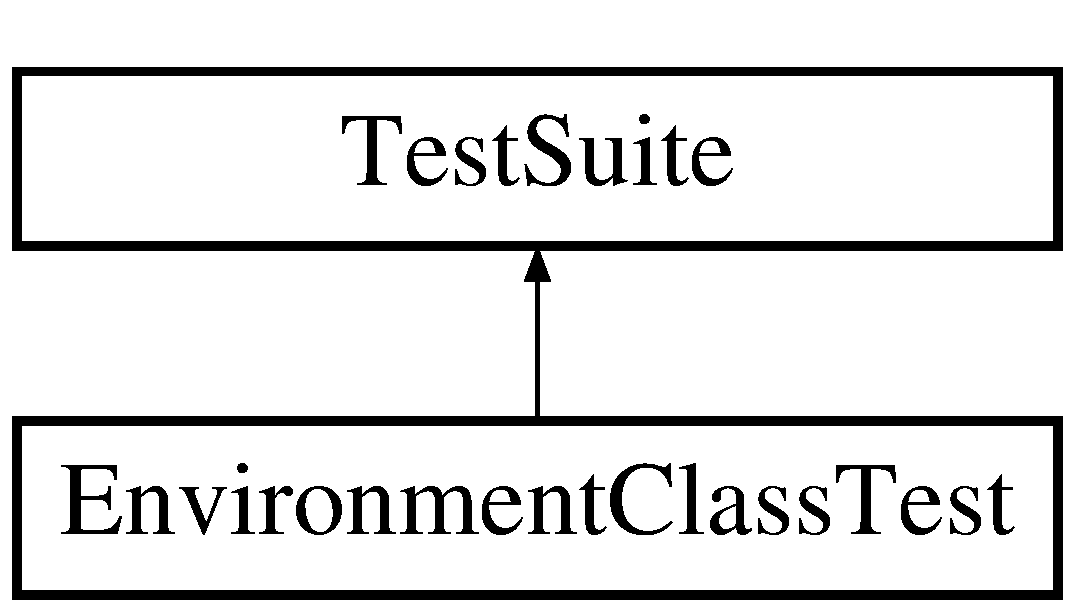
\includegraphics[height=2.000000cm]{classEnvironmentClassTest}
\end{center}
\end{figure}
\subsection*{Public Member Functions}
\begin{DoxyCompactItemize}
\item 
void \hyperlink{classEnvironmentClassTest_aea6f1c71d57ae40bf3fc7d096cf561a8}{Test\-\_\-\-Homing\-Sensor\-Reading\-\_\-up\-Leftor\-Right} (void)
\begin{DoxyCompactList}\small\item\em When the target is at the direction of exactly up left, reset the \hyperlink{structNavigate}{Navigate}'s direction to 45. \end{DoxyCompactList}\item 
void \hyperlink{classEnvironmentClassTest_a80efcd90295b95510ffe4b966e905a9e}{Test\-\_\-\-Homing\-Sensor\-Reading\-\_\-down\-Leftor\-Right} (void)
\begin{DoxyCompactList}\small\item\em When the target is at the direction of exactly downright, reset the direction of \hyperlink{structNavigate}{Navigate} to 315, which is 360-\/315. \end{DoxyCompactList}\item 
void \hyperlink{classEnvironmentClassTest_a888d1566d66aafb04146c8eb3ef67084}{Test\-\_\-\-Homing\-Sensor\-Reading\-\_\-\-Up} (void)
\begin{DoxyCompactList}\small\item\em When the target is at the direction of exactly up, reset the direction of \hyperlink{structNavigate}{Navigate} to 90 degrees, which makes the direction to 90. \end{DoxyCompactList}\item 
void \hyperlink{classEnvironmentClassTest_ad775e188eeabf3f42cded2a7c12c1320}{Test\-\_\-\-Homing\-Sensor\-Reading\-\_\-down} (void)
\begin{DoxyCompactList}\small\item\em When the target is at the direction of exactly below, reset the direction of \hyperlink{structNavigate}{Navigate} to 270, which makes the robot points down. \end{DoxyCompactList}\item 
void \hyperlink{classEnvironmentClassTest_a4b2bed563687924d81ee47326e209ff5}{Test\-\_\-update\-\_\-collide\-\_\-other\-Obj\-\_\-\-Not\-\_\-\-Verticle\-\_\-below} (void)
\begin{DoxyCompactList}\small\item\em When the center of Obstacle is below the line drawn by the robot, and orientation of robot is between 0 and 90, decrement the orientation of robot by 90 degrees. \end{DoxyCompactList}\item 
void \hyperlink{classEnvironmentClassTest_a03c106d609ce4cc49cd522f976cd4954}{Test\-\_\-update\-\_\-collide\-\_\-other\-Obj\-\_\-\-Not\-\_\-\-Verticle\-\_\-hori} (void)
\begin{DoxyCompactList}\small\item\em When the center of Obstacle is at the same horizon with the line drawn by the robot, increment the orientation of robot by 180 degrees, which means make it move back. \end{DoxyCompactList}\item 
void \hyperlink{classEnvironmentClassTest_a4a6193973d424e61be7b0c1a2d3f09ad}{Test\-\_\-update\-\_\-collide\-\_\-other\-Obj\-\_\-\-Not\-\_\-\-Verticle\-\_\-above} (void)
\begin{DoxyCompactList}\small\item\em When the center of Obstacle is above the line drawn by the robot, and orientation is between 0 and 90, decrement the orientation of robot by 90 degrees. \end{DoxyCompactList}\item 
void \hyperlink{classEnvironmentClassTest_ad2ac784ce8639415ead66cb3e1ab09e9}{Test\-\_\-update\-\_\-collide\-\_\-other\-Obj\-\_\-\-Verticle\-\_\-right} (void)
\begin{DoxyCompactList}\small\item\em When the center of Obstacle is to the right of the line drawn by the robot, and the orientaion of robot is 270, which means moving downwards, decrement the orientation by 90 degrees. \end{DoxyCompactList}\item 
void \hyperlink{classEnvironmentClassTest_aae3e2db645184add94f5735d2f0b25e6}{Test\-\_\-update\-\_\-collide\-\_\-other\-Obj\-\_\-\-Verticle\-\_\-left} (void)
\begin{DoxyCompactList}\small\item\em When the center of Obstacle is to the left of the line drawn by the robot, and orientation is 90, which means moving upwards, decrement the orientation of robot by 90 degrees. \end{DoxyCompactList}\item 
void \hyperlink{classEnvironmentClassTest_a6c143d7020eeb3ee83591606bcb3eca0}{Test\-\_\-update\-\_\-collide\-\_\-other\-Obj\-\_\-\-Verticle\-\_\-\-Ver} (void)
\begin{DoxyCompactList}\small\item\em When the center of Obstacle is on the line drawn by the robot, and the robot is moving vertically, decrement the orientation of robot by 180. \end{DoxyCompactList}\item 
void \hyperlink{classEnvironmentClassTest_a202238e6bec3a80f625519c9d1658c59}{Test\-\_\-updatecollide\-\_\-top\-\_\-turn\-\_\-right} (void)
\begin{DoxyCompactList}\small\item\em The following 8 test cases are to detect collision with Wall. For this function, it tests when the orientatioin is between 0 and 90, and it touched the top wall, it's orientation will decrement by 90. \end{DoxyCompactList}\item 
void \hyperlink{classEnvironmentClassTest_a0e29ad516c2ac19f2388dd1e9989dd90}{Test\-\_\-update\-\_\-collide\-\_\-top\-\_\-turn\-\_\-left} (void)
\begin{DoxyCompactList}\small\item\em For this function, it tests when the orientatioin is between 90 and 180, and it touched the top wall, it's orientation will increment by 90. \end{DoxyCompactList}\item 
void \hyperlink{classEnvironmentClassTest_ad739326d2fd1e2d91ebbaa4f05d3a5d0}{Test\-\_\-update\-\_\-collide\-\_\-bottom\-\_\-turn\-\_\-right} (void)
\begin{DoxyCompactList}\small\item\em For this function, it tests when the orientatioin is between 180 and 270, and it touched the bottom wall, it's orientation will decrement by 90. \end{DoxyCompactList}\item 
void \hyperlink{classEnvironmentClassTest_a18a7de3e61196c4cee5c3d0c4678aee5}{Test\-\_\-update\-\_\-collide\-\_\-bottom\-\_\-turn\-\_\-left} (void)
\begin{DoxyCompactList}\small\item\em For this function, it tests when the orientatioin is between 180 and 360, and it touched the bottom wall, it's orientation will decrement by 90. \end{DoxyCompactList}\item 
void \hyperlink{classEnvironmentClassTest_a8115b7b021e30fd0e449e2a69d7a30ee}{Test\-\_\-update\-\_\-collide\-\_\-left\-\_\-turn\-\_\-right} (void)
\begin{DoxyCompactList}\small\item\em For this function, it tests when the orientatioin is between 90 and 180, and it touched the right wall, it's orientation will decrement by 90. \end{DoxyCompactList}\item 
void \hyperlink{classEnvironmentClassTest_a41ebe9e2605a503fe5865c2ecdbfd8e4}{Test\-\_\-update\-\_\-collide\-\_\-left\-\_\-turn\-\_\-left} (void)
\begin{DoxyCompactList}\small\item\em For this function, it tests when the orientatioin is between 180 and 270, and it touched the right wall, it's orientation will increment by 90. \end{DoxyCompactList}\item 
void \hyperlink{classEnvironmentClassTest_a27d199a25c9ba79cd8b58bdaf5e899ba}{Test\-\_\-update\-\_\-collide\-\_\-right\-\_\-turn\-\_\-right} (void)
\begin{DoxyCompactList}\small\item\em For this function, it tests when the orientatioin is between 270 and 360, and it touched the right wall, it's orientation will decrement by 90. \end{DoxyCompactList}\item 
void \hyperlink{classEnvironmentClassTest_ab276ec81cc77f81538ce49bb3234066a}{Test\-\_\-update\-\_\-collide\-\_\-right\-\_\-turn\-\_\-left} (void)
\begin{DoxyCompactList}\small\item\em For this function, it tests when the orientatioin is between 0 and 90, and it touched the right wall, it's orientation will increment by 90. \end{DoxyCompactList}\item 
void \hyperlink{classEnvironmentClassTest_a3f5427ee507cef27351aebccef508a3c}{Test\-\_\-get\-Count} ()
\begin{DoxyCompactList}\small\item\em When there's one object registered, get\-Count() function return 1. \end{DoxyCompactList}\item 
void \hyperlink{classEnvironmentClassTest_ad0f5791ae30997ba0264f5c8b29d67b0}{Test\-\_\-register\-Object} (\hyperlink{classObject}{Object} obj)
\begin{DoxyCompactList}\small\item\em To test that when two objects are registered, get\-Count() function returns two. \end{DoxyCompactList}\item 
void \hyperlink{classEnvironmentClassTest_aa56cb296aa9b61bf5fff62815fa320ea}{Test\-\_\-touch\-Sensor\-Reading\-\_\-find\-\_\-target} (\hyperlink{classObject}{Object} obj)
\begin{DoxyCompactList}\small\item\em When the target is found, the status marked is 1. \end{DoxyCompactList}\item 
void \hyperlink{classEnvironmentClassTest_ab33d3a63cd4f5b8669788f50d37fb2ce}{Test\-\_\-touchsensor\-Reading\-\_\-find\-\_\-self} (\hyperlink{classObject}{Object} obj)
\begin{DoxyCompactList}\small\item\em When there is only one object and it's Robot, the robot would find itself, so the status is marked as 0. \end{DoxyCompactList}\item 
void \hyperlink{classEnvironmentClassTest_a7efc73377aef53781c7130fd80088c5d}{Test\-\_\-touch\-Sensor\-Reading\-\_\-detect\-\_\-wall} (\hyperlink{classObject}{Object} obj)
\begin{DoxyCompactList}\small\item\em When wall is detected, the status is marked ad 3. \end{DoxyCompactList}\item 
void \hyperlink{classEnvironmentClassTest_a43fff8a75f5a49a83b987ad96aa13897}{Test\-\_\-touch\-Sensor\-Reading\-\_\-find\-\_\-other\-\_\-object} (\hyperlink{classObject}{Object} obj)
\begin{DoxyCompactList}\small\item\em When Robot finds other objects, the status is marked as 2. \end{DoxyCompactList}\item 
void \hyperlink{classEnvironmentClassTest_adc618d79e098a26b928925ce11609e6f}{Test\-\_\-update\-\_\-\-Find\-\_\-\-Target} (void)
\begin{DoxyCompactList}\small\item\em When one is Target, other is not, and collision detected, decrements the objects count by 2. \end{DoxyCompactList}\item 
void \hyperlink{classEnvironmentClassTest_a32e8d69d217c911bc60e56f512be4e04}{Test\-\_\-update\-\_\-\-No\-\_\-\-Collision} (void)
\begin{DoxyCompactList}\small\item\em This test case is to test when there is no collision, the orientation of robot keeps unchanges. \end{DoxyCompactList}\end{DoxyCompactItemize}


\subsection{Member Function Documentation}
\hypertarget{classEnvironmentClassTest_a3f5427ee507cef27351aebccef508a3c}{\index{Environment\-Class\-Test@{Environment\-Class\-Test}!Test\-\_\-get\-Count@{Test\-\_\-get\-Count}}
\index{Test\-\_\-get\-Count@{Test\-\_\-get\-Count}!EnvironmentClassTest@{Environment\-Class\-Test}}
\subsubsection[{Test\-\_\-get\-Count}]{\setlength{\rightskip}{0pt plus 5cm}void Environment\-Class\-Test\-::\-Test\-\_\-get\-Count (
\begin{DoxyParamCaption}
{}
\end{DoxyParamCaption}
)\hspace{0.3cm}{\ttfamily [inline]}}}\label{classEnvironmentClassTest_a3f5427ee507cef27351aebccef508a3c}


When there's one object registered, get\-Count() function return 1. 


\begin{DoxyParams}{Parameters}
{\em void} & \\
\hline
\end{DoxyParams}
\hypertarget{classEnvironmentClassTest_ad775e188eeabf3f42cded2a7c12c1320}{\index{Environment\-Class\-Test@{Environment\-Class\-Test}!Test\-\_\-\-Homing\-Sensor\-Reading\-\_\-down@{Test\-\_\-\-Homing\-Sensor\-Reading\-\_\-down}}
\index{Test\-\_\-\-Homing\-Sensor\-Reading\-\_\-down@{Test\-\_\-\-Homing\-Sensor\-Reading\-\_\-down}!EnvironmentClassTest@{Environment\-Class\-Test}}
\subsubsection[{Test\-\_\-\-Homing\-Sensor\-Reading\-\_\-down}]{\setlength{\rightskip}{0pt plus 5cm}void Environment\-Class\-Test\-::\-Test\-\_\-\-Homing\-Sensor\-Reading\-\_\-down (
\begin{DoxyParamCaption}
\item[{void}]{}
\end{DoxyParamCaption}
)\hspace{0.3cm}{\ttfamily [inline]}}}\label{classEnvironmentClassTest_ad775e188eeabf3f42cded2a7c12c1320}


When the target is at the direction of exactly below, reset the direction of \hyperlink{structNavigate}{Navigate} to 270, which makes the robot points down. 


\begin{DoxyParams}{Parameters}
{\em void} & \\
\hline
\end{DoxyParams}
\hypertarget{classEnvironmentClassTest_a80efcd90295b95510ffe4b966e905a9e}{\index{Environment\-Class\-Test@{Environment\-Class\-Test}!Test\-\_\-\-Homing\-Sensor\-Reading\-\_\-down\-Leftor\-Right@{Test\-\_\-\-Homing\-Sensor\-Reading\-\_\-down\-Leftor\-Right}}
\index{Test\-\_\-\-Homing\-Sensor\-Reading\-\_\-down\-Leftor\-Right@{Test\-\_\-\-Homing\-Sensor\-Reading\-\_\-down\-Leftor\-Right}!EnvironmentClassTest@{Environment\-Class\-Test}}
\subsubsection[{Test\-\_\-\-Homing\-Sensor\-Reading\-\_\-down\-Leftor\-Right}]{\setlength{\rightskip}{0pt plus 5cm}void Environment\-Class\-Test\-::\-Test\-\_\-\-Homing\-Sensor\-Reading\-\_\-down\-Leftor\-Right (
\begin{DoxyParamCaption}
\item[{void}]{}
\end{DoxyParamCaption}
)\hspace{0.3cm}{\ttfamily [inline]}}}\label{classEnvironmentClassTest_a80efcd90295b95510ffe4b966e905a9e}


When the target is at the direction of exactly downright, reset the direction of \hyperlink{structNavigate}{Navigate} to 315, which is 360-\/315. 


\begin{DoxyParams}{Parameters}
{\em void} & \\
\hline
\end{DoxyParams}
\hypertarget{classEnvironmentClassTest_a888d1566d66aafb04146c8eb3ef67084}{\index{Environment\-Class\-Test@{Environment\-Class\-Test}!Test\-\_\-\-Homing\-Sensor\-Reading\-\_\-\-Up@{Test\-\_\-\-Homing\-Sensor\-Reading\-\_\-\-Up}}
\index{Test\-\_\-\-Homing\-Sensor\-Reading\-\_\-\-Up@{Test\-\_\-\-Homing\-Sensor\-Reading\-\_\-\-Up}!EnvironmentClassTest@{Environment\-Class\-Test}}
\subsubsection[{Test\-\_\-\-Homing\-Sensor\-Reading\-\_\-\-Up}]{\setlength{\rightskip}{0pt plus 5cm}void Environment\-Class\-Test\-::\-Test\-\_\-\-Homing\-Sensor\-Reading\-\_\-\-Up (
\begin{DoxyParamCaption}
\item[{void}]{}
\end{DoxyParamCaption}
)\hspace{0.3cm}{\ttfamily [inline]}}}\label{classEnvironmentClassTest_a888d1566d66aafb04146c8eb3ef67084}


When the target is at the direction of exactly up, reset the direction of \hyperlink{structNavigate}{Navigate} to 90 degrees, which makes the direction to 90. 


\begin{DoxyParams}{Parameters}
{\em void} & \\
\hline
\end{DoxyParams}
\hypertarget{classEnvironmentClassTest_aea6f1c71d57ae40bf3fc7d096cf561a8}{\index{Environment\-Class\-Test@{Environment\-Class\-Test}!Test\-\_\-\-Homing\-Sensor\-Reading\-\_\-up\-Leftor\-Right@{Test\-\_\-\-Homing\-Sensor\-Reading\-\_\-up\-Leftor\-Right}}
\index{Test\-\_\-\-Homing\-Sensor\-Reading\-\_\-up\-Leftor\-Right@{Test\-\_\-\-Homing\-Sensor\-Reading\-\_\-up\-Leftor\-Right}!EnvironmentClassTest@{Environment\-Class\-Test}}
\subsubsection[{Test\-\_\-\-Homing\-Sensor\-Reading\-\_\-up\-Leftor\-Right}]{\setlength{\rightskip}{0pt plus 5cm}void Environment\-Class\-Test\-::\-Test\-\_\-\-Homing\-Sensor\-Reading\-\_\-up\-Leftor\-Right (
\begin{DoxyParamCaption}
\item[{void}]{}
\end{DoxyParamCaption}
)\hspace{0.3cm}{\ttfamily [inline]}}}\label{classEnvironmentClassTest_aea6f1c71d57ae40bf3fc7d096cf561a8}


When the target is at the direction of exactly up left, reset the \hyperlink{structNavigate}{Navigate}'s direction to 45. 


\begin{DoxyParams}{Parameters}
{\em void} & \\
\hline
\end{DoxyParams}
\hypertarget{classEnvironmentClassTest_ad0f5791ae30997ba0264f5c8b29d67b0}{\index{Environment\-Class\-Test@{Environment\-Class\-Test}!Test\-\_\-register\-Object@{Test\-\_\-register\-Object}}
\index{Test\-\_\-register\-Object@{Test\-\_\-register\-Object}!EnvironmentClassTest@{Environment\-Class\-Test}}
\subsubsection[{Test\-\_\-register\-Object}]{\setlength{\rightskip}{0pt plus 5cm}void Environment\-Class\-Test\-::\-Test\-\_\-register\-Object (
\begin{DoxyParamCaption}
\item[{{\bf Object}}]{obj}
\end{DoxyParamCaption}
)\hspace{0.3cm}{\ttfamily [inline]}}}\label{classEnvironmentClassTest_ad0f5791ae30997ba0264f5c8b29d67b0}


To test that when two objects are registered, get\-Count() function returns two. 


\begin{DoxyParams}{Parameters}
{\em void} & \\
\hline
\end{DoxyParams}
\hypertarget{classEnvironmentClassTest_a7efc73377aef53781c7130fd80088c5d}{\index{Environment\-Class\-Test@{Environment\-Class\-Test}!Test\-\_\-touch\-Sensor\-Reading\-\_\-detect\-\_\-wall@{Test\-\_\-touch\-Sensor\-Reading\-\_\-detect\-\_\-wall}}
\index{Test\-\_\-touch\-Sensor\-Reading\-\_\-detect\-\_\-wall@{Test\-\_\-touch\-Sensor\-Reading\-\_\-detect\-\_\-wall}!EnvironmentClassTest@{Environment\-Class\-Test}}
\subsubsection[{Test\-\_\-touch\-Sensor\-Reading\-\_\-detect\-\_\-wall}]{\setlength{\rightskip}{0pt plus 5cm}void Environment\-Class\-Test\-::\-Test\-\_\-touch\-Sensor\-Reading\-\_\-detect\-\_\-wall (
\begin{DoxyParamCaption}
\item[{{\bf Object}}]{obj}
\end{DoxyParamCaption}
)\hspace{0.3cm}{\ttfamily [inline]}}}\label{classEnvironmentClassTest_a7efc73377aef53781c7130fd80088c5d}


When wall is detected, the status is marked ad 3. 


\begin{DoxyParams}{Parameters}
{\em void} & \\
\hline
\end{DoxyParams}
\hypertarget{classEnvironmentClassTest_a43fff8a75f5a49a83b987ad96aa13897}{\index{Environment\-Class\-Test@{Environment\-Class\-Test}!Test\-\_\-touch\-Sensor\-Reading\-\_\-find\-\_\-other\-\_\-object@{Test\-\_\-touch\-Sensor\-Reading\-\_\-find\-\_\-other\-\_\-object}}
\index{Test\-\_\-touch\-Sensor\-Reading\-\_\-find\-\_\-other\-\_\-object@{Test\-\_\-touch\-Sensor\-Reading\-\_\-find\-\_\-other\-\_\-object}!EnvironmentClassTest@{Environment\-Class\-Test}}
\subsubsection[{Test\-\_\-touch\-Sensor\-Reading\-\_\-find\-\_\-other\-\_\-object}]{\setlength{\rightskip}{0pt plus 5cm}void Environment\-Class\-Test\-::\-Test\-\_\-touch\-Sensor\-Reading\-\_\-find\-\_\-other\-\_\-object (
\begin{DoxyParamCaption}
\item[{{\bf Object}}]{obj}
\end{DoxyParamCaption}
)\hspace{0.3cm}{\ttfamily [inline]}}}\label{classEnvironmentClassTest_a43fff8a75f5a49a83b987ad96aa13897}


When Robot finds other objects, the status is marked as 2. 


\begin{DoxyParams}{Parameters}
{\em void} & \\
\hline
\end{DoxyParams}
\hypertarget{classEnvironmentClassTest_ab33d3a63cd4f5b8669788f50d37fb2ce}{\index{Environment\-Class\-Test@{Environment\-Class\-Test}!Test\-\_\-touchsensor\-Reading\-\_\-find\-\_\-self@{Test\-\_\-touchsensor\-Reading\-\_\-find\-\_\-self}}
\index{Test\-\_\-touchsensor\-Reading\-\_\-find\-\_\-self@{Test\-\_\-touchsensor\-Reading\-\_\-find\-\_\-self}!EnvironmentClassTest@{Environment\-Class\-Test}}
\subsubsection[{Test\-\_\-touchsensor\-Reading\-\_\-find\-\_\-self}]{\setlength{\rightskip}{0pt plus 5cm}void Environment\-Class\-Test\-::\-Test\-\_\-touchsensor\-Reading\-\_\-find\-\_\-self (
\begin{DoxyParamCaption}
\item[{{\bf Object}}]{obj}
\end{DoxyParamCaption}
)\hspace{0.3cm}{\ttfamily [inline]}}}\label{classEnvironmentClassTest_ab33d3a63cd4f5b8669788f50d37fb2ce}


When there is only one object and it's Robot, the robot would find itself, so the status is marked as 0. 


\begin{DoxyParams}{Parameters}
{\em void} & \\
\hline
\end{DoxyParams}
\hypertarget{classEnvironmentClassTest_aa56cb296aa9b61bf5fff62815fa320ea}{\index{Environment\-Class\-Test@{Environment\-Class\-Test}!Test\-\_\-touch\-Sensor\-Reading\-\_\-find\-\_\-target@{Test\-\_\-touch\-Sensor\-Reading\-\_\-find\-\_\-target}}
\index{Test\-\_\-touch\-Sensor\-Reading\-\_\-find\-\_\-target@{Test\-\_\-touch\-Sensor\-Reading\-\_\-find\-\_\-target}!EnvironmentClassTest@{Environment\-Class\-Test}}
\subsubsection[{Test\-\_\-touch\-Sensor\-Reading\-\_\-find\-\_\-target}]{\setlength{\rightskip}{0pt plus 5cm}void Environment\-Class\-Test\-::\-Test\-\_\-touch\-Sensor\-Reading\-\_\-find\-\_\-target (
\begin{DoxyParamCaption}
\item[{{\bf Object}}]{obj}
\end{DoxyParamCaption}
)\hspace{0.3cm}{\ttfamily [inline]}}}\label{classEnvironmentClassTest_aa56cb296aa9b61bf5fff62815fa320ea}


When the target is found, the status marked is 1. 


\begin{DoxyParams}{Parameters}
{\em void} & \\
\hline
\end{DoxyParams}
\hypertarget{classEnvironmentClassTest_a18a7de3e61196c4cee5c3d0c4678aee5}{\index{Environment\-Class\-Test@{Environment\-Class\-Test}!Test\-\_\-update\-\_\-collide\-\_\-bottom\-\_\-turn\-\_\-left@{Test\-\_\-update\-\_\-collide\-\_\-bottom\-\_\-turn\-\_\-left}}
\index{Test\-\_\-update\-\_\-collide\-\_\-bottom\-\_\-turn\-\_\-left@{Test\-\_\-update\-\_\-collide\-\_\-bottom\-\_\-turn\-\_\-left}!EnvironmentClassTest@{Environment\-Class\-Test}}
\subsubsection[{Test\-\_\-update\-\_\-collide\-\_\-bottom\-\_\-turn\-\_\-left}]{\setlength{\rightskip}{0pt plus 5cm}void Environment\-Class\-Test\-::\-Test\-\_\-update\-\_\-collide\-\_\-bottom\-\_\-turn\-\_\-left (
\begin{DoxyParamCaption}
\item[{void}]{}
\end{DoxyParamCaption}
)\hspace{0.3cm}{\ttfamily [inline]}}}\label{classEnvironmentClassTest_a18a7de3e61196c4cee5c3d0c4678aee5}


For this function, it tests when the orientatioin is between 180 and 360, and it touched the bottom wall, it's orientation will decrement by 90. 


\begin{DoxyParams}{Parameters}
{\em void} & \\
\hline
\end{DoxyParams}
\hypertarget{classEnvironmentClassTest_ad739326d2fd1e2d91ebbaa4f05d3a5d0}{\index{Environment\-Class\-Test@{Environment\-Class\-Test}!Test\-\_\-update\-\_\-collide\-\_\-bottom\-\_\-turn\-\_\-right@{Test\-\_\-update\-\_\-collide\-\_\-bottom\-\_\-turn\-\_\-right}}
\index{Test\-\_\-update\-\_\-collide\-\_\-bottom\-\_\-turn\-\_\-right@{Test\-\_\-update\-\_\-collide\-\_\-bottom\-\_\-turn\-\_\-right}!EnvironmentClassTest@{Environment\-Class\-Test}}
\subsubsection[{Test\-\_\-update\-\_\-collide\-\_\-bottom\-\_\-turn\-\_\-right}]{\setlength{\rightskip}{0pt plus 5cm}void Environment\-Class\-Test\-::\-Test\-\_\-update\-\_\-collide\-\_\-bottom\-\_\-turn\-\_\-right (
\begin{DoxyParamCaption}
\item[{void}]{}
\end{DoxyParamCaption}
)\hspace{0.3cm}{\ttfamily [inline]}}}\label{classEnvironmentClassTest_ad739326d2fd1e2d91ebbaa4f05d3a5d0}


For this function, it tests when the orientatioin is between 180 and 270, and it touched the bottom wall, it's orientation will decrement by 90. 


\begin{DoxyParams}{Parameters}
{\em void} & \\
\hline
\end{DoxyParams}
\hypertarget{classEnvironmentClassTest_a41ebe9e2605a503fe5865c2ecdbfd8e4}{\index{Environment\-Class\-Test@{Environment\-Class\-Test}!Test\-\_\-update\-\_\-collide\-\_\-left\-\_\-turn\-\_\-left@{Test\-\_\-update\-\_\-collide\-\_\-left\-\_\-turn\-\_\-left}}
\index{Test\-\_\-update\-\_\-collide\-\_\-left\-\_\-turn\-\_\-left@{Test\-\_\-update\-\_\-collide\-\_\-left\-\_\-turn\-\_\-left}!EnvironmentClassTest@{Environment\-Class\-Test}}
\subsubsection[{Test\-\_\-update\-\_\-collide\-\_\-left\-\_\-turn\-\_\-left}]{\setlength{\rightskip}{0pt plus 5cm}void Environment\-Class\-Test\-::\-Test\-\_\-update\-\_\-collide\-\_\-left\-\_\-turn\-\_\-left (
\begin{DoxyParamCaption}
\item[{void}]{}
\end{DoxyParamCaption}
)\hspace{0.3cm}{\ttfamily [inline]}}}\label{classEnvironmentClassTest_a41ebe9e2605a503fe5865c2ecdbfd8e4}


For this function, it tests when the orientatioin is between 180 and 270, and it touched the right wall, it's orientation will increment by 90. 


\begin{DoxyParams}{Parameters}
{\em void} & \\
\hline
\end{DoxyParams}
\hypertarget{classEnvironmentClassTest_a8115b7b021e30fd0e449e2a69d7a30ee}{\index{Environment\-Class\-Test@{Environment\-Class\-Test}!Test\-\_\-update\-\_\-collide\-\_\-left\-\_\-turn\-\_\-right@{Test\-\_\-update\-\_\-collide\-\_\-left\-\_\-turn\-\_\-right}}
\index{Test\-\_\-update\-\_\-collide\-\_\-left\-\_\-turn\-\_\-right@{Test\-\_\-update\-\_\-collide\-\_\-left\-\_\-turn\-\_\-right}!EnvironmentClassTest@{Environment\-Class\-Test}}
\subsubsection[{Test\-\_\-update\-\_\-collide\-\_\-left\-\_\-turn\-\_\-right}]{\setlength{\rightskip}{0pt plus 5cm}void Environment\-Class\-Test\-::\-Test\-\_\-update\-\_\-collide\-\_\-left\-\_\-turn\-\_\-right (
\begin{DoxyParamCaption}
\item[{void}]{}
\end{DoxyParamCaption}
)\hspace{0.3cm}{\ttfamily [inline]}}}\label{classEnvironmentClassTest_a8115b7b021e30fd0e449e2a69d7a30ee}


For this function, it tests when the orientatioin is between 90 and 180, and it touched the right wall, it's orientation will decrement by 90. 


\begin{DoxyParams}{Parameters}
{\em void} & \\
\hline
\end{DoxyParams}
\hypertarget{classEnvironmentClassTest_a4a6193973d424e61be7b0c1a2d3f09ad}{\index{Environment\-Class\-Test@{Environment\-Class\-Test}!Test\-\_\-update\-\_\-collide\-\_\-other\-Obj\-\_\-\-Not\-\_\-\-Verticle\-\_\-above@{Test\-\_\-update\-\_\-collide\-\_\-other\-Obj\-\_\-\-Not\-\_\-\-Verticle\-\_\-above}}
\index{Test\-\_\-update\-\_\-collide\-\_\-other\-Obj\-\_\-\-Not\-\_\-\-Verticle\-\_\-above@{Test\-\_\-update\-\_\-collide\-\_\-other\-Obj\-\_\-\-Not\-\_\-\-Verticle\-\_\-above}!EnvironmentClassTest@{Environment\-Class\-Test}}
\subsubsection[{Test\-\_\-update\-\_\-collide\-\_\-other\-Obj\-\_\-\-Not\-\_\-\-Verticle\-\_\-above}]{\setlength{\rightskip}{0pt plus 5cm}void Environment\-Class\-Test\-::\-Test\-\_\-update\-\_\-collide\-\_\-other\-Obj\-\_\-\-Not\-\_\-\-Verticle\-\_\-above (
\begin{DoxyParamCaption}
\item[{void}]{}
\end{DoxyParamCaption}
)\hspace{0.3cm}{\ttfamily [inline]}}}\label{classEnvironmentClassTest_a4a6193973d424e61be7b0c1a2d3f09ad}


When the center of Obstacle is above the line drawn by the robot, and orientation is between 0 and 90, decrement the orientation of robot by 90 degrees. 


\begin{DoxyParams}{Parameters}
{\em void} & \\
\hline
\end{DoxyParams}
\hypertarget{classEnvironmentClassTest_a4b2bed563687924d81ee47326e209ff5}{\index{Environment\-Class\-Test@{Environment\-Class\-Test}!Test\-\_\-update\-\_\-collide\-\_\-other\-Obj\-\_\-\-Not\-\_\-\-Verticle\-\_\-below@{Test\-\_\-update\-\_\-collide\-\_\-other\-Obj\-\_\-\-Not\-\_\-\-Verticle\-\_\-below}}
\index{Test\-\_\-update\-\_\-collide\-\_\-other\-Obj\-\_\-\-Not\-\_\-\-Verticle\-\_\-below@{Test\-\_\-update\-\_\-collide\-\_\-other\-Obj\-\_\-\-Not\-\_\-\-Verticle\-\_\-below}!EnvironmentClassTest@{Environment\-Class\-Test}}
\subsubsection[{Test\-\_\-update\-\_\-collide\-\_\-other\-Obj\-\_\-\-Not\-\_\-\-Verticle\-\_\-below}]{\setlength{\rightskip}{0pt plus 5cm}void Environment\-Class\-Test\-::\-Test\-\_\-update\-\_\-collide\-\_\-other\-Obj\-\_\-\-Not\-\_\-\-Verticle\-\_\-below (
\begin{DoxyParamCaption}
\item[{void}]{}
\end{DoxyParamCaption}
)\hspace{0.3cm}{\ttfamily [inline]}}}\label{classEnvironmentClassTest_a4b2bed563687924d81ee47326e209ff5}


When the center of Obstacle is below the line drawn by the robot, and orientation of robot is between 0 and 90, decrement the orientation of robot by 90 degrees. 


\begin{DoxyParams}{Parameters}
{\em void} & \\
\hline
\end{DoxyParams}
\hypertarget{classEnvironmentClassTest_a03c106d609ce4cc49cd522f976cd4954}{\index{Environment\-Class\-Test@{Environment\-Class\-Test}!Test\-\_\-update\-\_\-collide\-\_\-other\-Obj\-\_\-\-Not\-\_\-\-Verticle\-\_\-hori@{Test\-\_\-update\-\_\-collide\-\_\-other\-Obj\-\_\-\-Not\-\_\-\-Verticle\-\_\-hori}}
\index{Test\-\_\-update\-\_\-collide\-\_\-other\-Obj\-\_\-\-Not\-\_\-\-Verticle\-\_\-hori@{Test\-\_\-update\-\_\-collide\-\_\-other\-Obj\-\_\-\-Not\-\_\-\-Verticle\-\_\-hori}!EnvironmentClassTest@{Environment\-Class\-Test}}
\subsubsection[{Test\-\_\-update\-\_\-collide\-\_\-other\-Obj\-\_\-\-Not\-\_\-\-Verticle\-\_\-hori}]{\setlength{\rightskip}{0pt plus 5cm}void Environment\-Class\-Test\-::\-Test\-\_\-update\-\_\-collide\-\_\-other\-Obj\-\_\-\-Not\-\_\-\-Verticle\-\_\-hori (
\begin{DoxyParamCaption}
\item[{void}]{}
\end{DoxyParamCaption}
)\hspace{0.3cm}{\ttfamily [inline]}}}\label{classEnvironmentClassTest_a03c106d609ce4cc49cd522f976cd4954}


When the center of Obstacle is at the same horizon with the line drawn by the robot, increment the orientation of robot by 180 degrees, which means make it move back. 


\begin{DoxyParams}{Parameters}
{\em void} & \\
\hline
\end{DoxyParams}
\hypertarget{classEnvironmentClassTest_aae3e2db645184add94f5735d2f0b25e6}{\index{Environment\-Class\-Test@{Environment\-Class\-Test}!Test\-\_\-update\-\_\-collide\-\_\-other\-Obj\-\_\-\-Verticle\-\_\-left@{Test\-\_\-update\-\_\-collide\-\_\-other\-Obj\-\_\-\-Verticle\-\_\-left}}
\index{Test\-\_\-update\-\_\-collide\-\_\-other\-Obj\-\_\-\-Verticle\-\_\-left@{Test\-\_\-update\-\_\-collide\-\_\-other\-Obj\-\_\-\-Verticle\-\_\-left}!EnvironmentClassTest@{Environment\-Class\-Test}}
\subsubsection[{Test\-\_\-update\-\_\-collide\-\_\-other\-Obj\-\_\-\-Verticle\-\_\-left}]{\setlength{\rightskip}{0pt plus 5cm}void Environment\-Class\-Test\-::\-Test\-\_\-update\-\_\-collide\-\_\-other\-Obj\-\_\-\-Verticle\-\_\-left (
\begin{DoxyParamCaption}
\item[{void}]{}
\end{DoxyParamCaption}
)\hspace{0.3cm}{\ttfamily [inline]}}}\label{classEnvironmentClassTest_aae3e2db645184add94f5735d2f0b25e6}


When the center of Obstacle is to the left of the line drawn by the robot, and orientation is 90, which means moving upwards, decrement the orientation of robot by 90 degrees. 


\begin{DoxyParams}{Parameters}
{\em void} & \\
\hline
\end{DoxyParams}
\hypertarget{classEnvironmentClassTest_ad2ac784ce8639415ead66cb3e1ab09e9}{\index{Environment\-Class\-Test@{Environment\-Class\-Test}!Test\-\_\-update\-\_\-collide\-\_\-other\-Obj\-\_\-\-Verticle\-\_\-right@{Test\-\_\-update\-\_\-collide\-\_\-other\-Obj\-\_\-\-Verticle\-\_\-right}}
\index{Test\-\_\-update\-\_\-collide\-\_\-other\-Obj\-\_\-\-Verticle\-\_\-right@{Test\-\_\-update\-\_\-collide\-\_\-other\-Obj\-\_\-\-Verticle\-\_\-right}!EnvironmentClassTest@{Environment\-Class\-Test}}
\subsubsection[{Test\-\_\-update\-\_\-collide\-\_\-other\-Obj\-\_\-\-Verticle\-\_\-right}]{\setlength{\rightskip}{0pt plus 5cm}void Environment\-Class\-Test\-::\-Test\-\_\-update\-\_\-collide\-\_\-other\-Obj\-\_\-\-Verticle\-\_\-right (
\begin{DoxyParamCaption}
\item[{void}]{}
\end{DoxyParamCaption}
)\hspace{0.3cm}{\ttfamily [inline]}}}\label{classEnvironmentClassTest_ad2ac784ce8639415ead66cb3e1ab09e9}


When the center of Obstacle is to the right of the line drawn by the robot, and the orientaion of robot is 270, which means moving downwards, decrement the orientation by 90 degrees. 


\begin{DoxyParams}{Parameters}
{\em void} & \\
\hline
\end{DoxyParams}
\hypertarget{classEnvironmentClassTest_a6c143d7020eeb3ee83591606bcb3eca0}{\index{Environment\-Class\-Test@{Environment\-Class\-Test}!Test\-\_\-update\-\_\-collide\-\_\-other\-Obj\-\_\-\-Verticle\-\_\-\-Ver@{Test\-\_\-update\-\_\-collide\-\_\-other\-Obj\-\_\-\-Verticle\-\_\-\-Ver}}
\index{Test\-\_\-update\-\_\-collide\-\_\-other\-Obj\-\_\-\-Verticle\-\_\-\-Ver@{Test\-\_\-update\-\_\-collide\-\_\-other\-Obj\-\_\-\-Verticle\-\_\-\-Ver}!EnvironmentClassTest@{Environment\-Class\-Test}}
\subsubsection[{Test\-\_\-update\-\_\-collide\-\_\-other\-Obj\-\_\-\-Verticle\-\_\-\-Ver}]{\setlength{\rightskip}{0pt plus 5cm}void Environment\-Class\-Test\-::\-Test\-\_\-update\-\_\-collide\-\_\-other\-Obj\-\_\-\-Verticle\-\_\-\-Ver (
\begin{DoxyParamCaption}
\item[{void}]{}
\end{DoxyParamCaption}
)\hspace{0.3cm}{\ttfamily [inline]}}}\label{classEnvironmentClassTest_a6c143d7020eeb3ee83591606bcb3eca0}


When the center of Obstacle is on the line drawn by the robot, and the robot is moving vertically, decrement the orientation of robot by 180. 


\begin{DoxyParams}{Parameters}
{\em void} & \\
\hline
\end{DoxyParams}
\hypertarget{classEnvironmentClassTest_ab276ec81cc77f81538ce49bb3234066a}{\index{Environment\-Class\-Test@{Environment\-Class\-Test}!Test\-\_\-update\-\_\-collide\-\_\-right\-\_\-turn\-\_\-left@{Test\-\_\-update\-\_\-collide\-\_\-right\-\_\-turn\-\_\-left}}
\index{Test\-\_\-update\-\_\-collide\-\_\-right\-\_\-turn\-\_\-left@{Test\-\_\-update\-\_\-collide\-\_\-right\-\_\-turn\-\_\-left}!EnvironmentClassTest@{Environment\-Class\-Test}}
\subsubsection[{Test\-\_\-update\-\_\-collide\-\_\-right\-\_\-turn\-\_\-left}]{\setlength{\rightskip}{0pt plus 5cm}void Environment\-Class\-Test\-::\-Test\-\_\-update\-\_\-collide\-\_\-right\-\_\-turn\-\_\-left (
\begin{DoxyParamCaption}
\item[{void}]{}
\end{DoxyParamCaption}
)\hspace{0.3cm}{\ttfamily [inline]}}}\label{classEnvironmentClassTest_ab276ec81cc77f81538ce49bb3234066a}


For this function, it tests when the orientatioin is between 0 and 90, and it touched the right wall, it's orientation will increment by 90. 


\begin{DoxyParams}{Parameters}
{\em void} & \\
\hline
\end{DoxyParams}
\hypertarget{classEnvironmentClassTest_a27d199a25c9ba79cd8b58bdaf5e899ba}{\index{Environment\-Class\-Test@{Environment\-Class\-Test}!Test\-\_\-update\-\_\-collide\-\_\-right\-\_\-turn\-\_\-right@{Test\-\_\-update\-\_\-collide\-\_\-right\-\_\-turn\-\_\-right}}
\index{Test\-\_\-update\-\_\-collide\-\_\-right\-\_\-turn\-\_\-right@{Test\-\_\-update\-\_\-collide\-\_\-right\-\_\-turn\-\_\-right}!EnvironmentClassTest@{Environment\-Class\-Test}}
\subsubsection[{Test\-\_\-update\-\_\-collide\-\_\-right\-\_\-turn\-\_\-right}]{\setlength{\rightskip}{0pt plus 5cm}void Environment\-Class\-Test\-::\-Test\-\_\-update\-\_\-collide\-\_\-right\-\_\-turn\-\_\-right (
\begin{DoxyParamCaption}
\item[{void}]{}
\end{DoxyParamCaption}
)\hspace{0.3cm}{\ttfamily [inline]}}}\label{classEnvironmentClassTest_a27d199a25c9ba79cd8b58bdaf5e899ba}


For this function, it tests when the orientatioin is between 270 and 360, and it touched the right wall, it's orientation will decrement by 90. 


\begin{DoxyParams}{Parameters}
{\em void} & \\
\hline
\end{DoxyParams}
\hypertarget{classEnvironmentClassTest_a0e29ad516c2ac19f2388dd1e9989dd90}{\index{Environment\-Class\-Test@{Environment\-Class\-Test}!Test\-\_\-update\-\_\-collide\-\_\-top\-\_\-turn\-\_\-left@{Test\-\_\-update\-\_\-collide\-\_\-top\-\_\-turn\-\_\-left}}
\index{Test\-\_\-update\-\_\-collide\-\_\-top\-\_\-turn\-\_\-left@{Test\-\_\-update\-\_\-collide\-\_\-top\-\_\-turn\-\_\-left}!EnvironmentClassTest@{Environment\-Class\-Test}}
\subsubsection[{Test\-\_\-update\-\_\-collide\-\_\-top\-\_\-turn\-\_\-left}]{\setlength{\rightskip}{0pt plus 5cm}void Environment\-Class\-Test\-::\-Test\-\_\-update\-\_\-collide\-\_\-top\-\_\-turn\-\_\-left (
\begin{DoxyParamCaption}
\item[{void}]{}
\end{DoxyParamCaption}
)\hspace{0.3cm}{\ttfamily [inline]}}}\label{classEnvironmentClassTest_a0e29ad516c2ac19f2388dd1e9989dd90}


For this function, it tests when the orientatioin is between 90 and 180, and it touched the top wall, it's orientation will increment by 90. 


\begin{DoxyParams}{Parameters}
{\em void} & \\
\hline
\end{DoxyParams}
\hypertarget{classEnvironmentClassTest_adc618d79e098a26b928925ce11609e6f}{\index{Environment\-Class\-Test@{Environment\-Class\-Test}!Test\-\_\-update\-\_\-\-Find\-\_\-\-Target@{Test\-\_\-update\-\_\-\-Find\-\_\-\-Target}}
\index{Test\-\_\-update\-\_\-\-Find\-\_\-\-Target@{Test\-\_\-update\-\_\-\-Find\-\_\-\-Target}!EnvironmentClassTest@{Environment\-Class\-Test}}
\subsubsection[{Test\-\_\-update\-\_\-\-Find\-\_\-\-Target}]{\setlength{\rightskip}{0pt plus 5cm}void Environment\-Class\-Test\-::\-Test\-\_\-update\-\_\-\-Find\-\_\-\-Target (
\begin{DoxyParamCaption}
\item[{void}]{}
\end{DoxyParamCaption}
)\hspace{0.3cm}{\ttfamily [inline]}}}\label{classEnvironmentClassTest_adc618d79e098a26b928925ce11609e6f}


When one is Target, other is not, and collision detected, decrements the objects count by 2. 


\begin{DoxyParams}{Parameters}
{\em void} & \\
\hline
\end{DoxyParams}
\hypertarget{classEnvironmentClassTest_a32e8d69d217c911bc60e56f512be4e04}{\index{Environment\-Class\-Test@{Environment\-Class\-Test}!Test\-\_\-update\-\_\-\-No\-\_\-\-Collision@{Test\-\_\-update\-\_\-\-No\-\_\-\-Collision}}
\index{Test\-\_\-update\-\_\-\-No\-\_\-\-Collision@{Test\-\_\-update\-\_\-\-No\-\_\-\-Collision}!EnvironmentClassTest@{Environment\-Class\-Test}}
\subsubsection[{Test\-\_\-update\-\_\-\-No\-\_\-\-Collision}]{\setlength{\rightskip}{0pt plus 5cm}void Environment\-Class\-Test\-::\-Test\-\_\-update\-\_\-\-No\-\_\-\-Collision (
\begin{DoxyParamCaption}
\item[{void}]{}
\end{DoxyParamCaption}
)\hspace{0.3cm}{\ttfamily [inline]}}}\label{classEnvironmentClassTest_a32e8d69d217c911bc60e56f512be4e04}


This test case is to test when there is no collision, the orientation of robot keeps unchanges. 


\begin{DoxyParams}{Parameters}
{\em void} & \\
\hline
\end{DoxyParams}
\hypertarget{classEnvironmentClassTest_a202238e6bec3a80f625519c9d1658c59}{\index{Environment\-Class\-Test@{Environment\-Class\-Test}!Test\-\_\-updatecollide\-\_\-top\-\_\-turn\-\_\-right@{Test\-\_\-updatecollide\-\_\-top\-\_\-turn\-\_\-right}}
\index{Test\-\_\-updatecollide\-\_\-top\-\_\-turn\-\_\-right@{Test\-\_\-updatecollide\-\_\-top\-\_\-turn\-\_\-right}!EnvironmentClassTest@{Environment\-Class\-Test}}
\subsubsection[{Test\-\_\-updatecollide\-\_\-top\-\_\-turn\-\_\-right}]{\setlength{\rightskip}{0pt plus 5cm}void Environment\-Class\-Test\-::\-Test\-\_\-updatecollide\-\_\-top\-\_\-turn\-\_\-right (
\begin{DoxyParamCaption}
\item[{void}]{}
\end{DoxyParamCaption}
)\hspace{0.3cm}{\ttfamily [inline]}}}\label{classEnvironmentClassTest_a202238e6bec3a80f625519c9d1658c59}


The following 8 test cases are to detect collision with Wall. For this function, it tests when the orientatioin is between 0 and 90, and it touched the top wall, it's orientation will decrement by 90. 


\begin{DoxyParams}{Parameters}
{\em void} & \\
\hline
\end{DoxyParams}


The documentation for this class was generated from the following file\-:\begin{DoxyCompactItemize}
\item 
\hyperlink{EnvironmentClassTest_8h}{Environment\-Class\-Test.\-h}\end{DoxyCompactItemize}

\hypertarget{structNavigate}{\section{Navigate Struct Reference}
\label{structNavigate}\index{Navigate@{Navigate}}
}


{\ttfamily \#include $<$Object.\-h$>$}

\subsection*{Public Attributes}
\begin{DoxyCompactItemize}
\item 
double \hyperlink{structNavigate_a44093df3edad183c340d85d9762a27f8}{delta\-Distance}
\item 
double \hyperlink{structNavigate_a245fd5044011a7d7d8471e52771bf4b3}{delta\-Ori}
\end{DoxyCompactItemize}


\subsection{Member Data Documentation}
\hypertarget{structNavigate_a44093df3edad183c340d85d9762a27f8}{\index{Navigate@{Navigate}!delta\-Distance@{delta\-Distance}}
\index{delta\-Distance@{delta\-Distance}!Navigate@{Navigate}}
\subsubsection[{delta\-Distance}]{\setlength{\rightskip}{0pt plus 5cm}double Navigate\-::delta\-Distance}}\label{structNavigate_a44093df3edad183c340d85d9762a27f8}
$<$ Vector including distance and orientation information that robot need to locate target \hypertarget{structNavigate_a245fd5044011a7d7d8471e52771bf4b3}{\index{Navigate@{Navigate}!delta\-Ori@{delta\-Ori}}
\index{delta\-Ori@{delta\-Ori}!Navigate@{Navigate}}
\subsubsection[{delta\-Ori}]{\setlength{\rightskip}{0pt plus 5cm}double Navigate\-::delta\-Ori}}\label{structNavigate_a245fd5044011a7d7d8471e52771bf4b3}


The documentation for this struct was generated from the following file\-:\begin{DoxyCompactItemize}
\item 
\hyperlink{Object_8h}{Object.\-h}\end{DoxyCompactItemize}

\hypertarget{classObject}{\section{Object Class Reference}
\label{classObject}\index{Object@{Object}}
}


Super Class of Robot\-Class, Target and Obstacle, contains position x, y and size.  




{\ttfamily \#include $<$Object.\-h$>$}

\subsection*{Public Member Functions}
\begin{DoxyCompactItemize}
\item 
\hyperlink{classObject_a40860402e64d8008fb42329df7097cdb}{Object} ()
\begin{DoxyCompactList}\small\item\em The default constructor. \end{DoxyCompactList}\item 
\hyperlink{classObject_a1578ef305ecdd88d8b2c0b4408d0f4f2}{Object} (double x, double y, double s, double sp, double ori, \hyperlink{Object_8h_a5a4538eeab397888d88a4eefcc5a1345}{Shape\-Type} sh, \hyperlink{Object_8h_a842c5e2e69277690b064bf363c017980}{Object\-Type} objtype, float c\mbox{[}3\mbox{]}, int id)
\begin{DoxyCompactList}\small\item\em A Constructor. \end{DoxyCompactList}\item 
\hyperlink{classObject_ae8f5483f459e46687bd01e6f9977afd3}{$\sim$\-Object} ()
\begin{DoxyCompactList}\small\item\em The default constructor. \end{DoxyCompactList}\item 
void \hyperlink{classObject_a20943e8303df77a63e7173b7cb31fcb4}{set\-Shape} (\hyperlink{Object_8h_a5a4538eeab397888d88a4eefcc5a1345}{Shape\-Type} shape)
\begin{DoxyCompactList}\small\item\em Set \hyperlink{classObject}{Object}'s shape through arguements. \end{DoxyCompactList}\item 
void \hyperlink{classObject_a24d288762ff0406ea1018ce0063c5636}{set\-Color} (float c\mbox{[}$\,$\mbox{]})
\begin{DoxyCompactList}\small\item\em Set \hyperlink{classObject}{Object}'s color through arguements. \end{DoxyCompactList}\item 
void \hyperlink{classObject_a91f40854ef8471bdc38d8b3848e3c25a}{set\-Type} (\hyperlink{Object_8h_a842c5e2e69277690b064bf363c017980}{Object\-Type} obj)
\begin{DoxyCompactList}\small\item\em Set \hyperlink{classObject}{Object}'s type through arguements. \end{DoxyCompactList}\item 
void \hyperlink{classObject_a31495a5948411e2cb7b10e2c211b2f9b}{set\-Position} (double x, double y)
\begin{DoxyCompactList}\small\item\em Set \hyperlink{classObject}{Object}'s Position through arguements. \end{DoxyCompactList}\item 
void \hyperlink{classObject_a0ade9aa73271d6ec7aa9bf6b0d458270}{set\-Size} (double s)
\begin{DoxyCompactList}\small\item\em set \hyperlink{classObject}{Object}'s size through arguement. \end{DoxyCompactList}\item 
double \hyperlink{classObject_a82313b69986eebc7e2dff3925e2684b2}{get\-X\-Position} ()
\begin{DoxyCompactList}\small\item\em Return current x position of \hyperlink{classObject}{Object}. \end{DoxyCompactList}\item 
double \hyperlink{classObject_aa2816e5e411b0bc1179a2762f7e2b552}{get\-Y\-Position} ()
\begin{DoxyCompactList}\small\item\em Return current y position of \hyperlink{classObject}{Object}. \end{DoxyCompactList}\item 
double \hyperlink{classObject_aa45378bcd52e52cae8070de90b2b1148}{get\-Size} ()
\begin{DoxyCompactList}\small\item\em Return current size of \hyperlink{classObject}{Object}. \end{DoxyCompactList}\item 
void \hyperlink{classObject_a9c0c9ea4d4168ba6775ec8d4ce0d980a}{set\-Orientation} (double degrees)
\begin{DoxyCompactList}\small\item\em Set \hyperlink{classObject}{Object}'s orientation through arguement. \end{DoxyCompactList}\item 
void \hyperlink{classObject_a68f33643bbd5fe7410f4f367433010b3}{set\-Speed} (double pps)
\begin{DoxyCompactList}\small\item\em set \hyperlink{classObject}{Object}'s speed through arguement. \end{DoxyCompactList}\item 
double \hyperlink{classObject_a138712103a66b8d7268ef839464a1262}{get\-Orientation} ()
\begin{DoxyCompactList}\small\item\em Return current orientation of \hyperlink{classObject}{Object}. \end{DoxyCompactList}\item 
double \hyperlink{classObject_a407ec2b4aaa93429355c58e8d4a3d138}{get\-Speed} ()
\begin{DoxyCompactList}\small\item\em Return current speed of \hyperlink{classObject}{Object}. \end{DoxyCompactList}\item 
\hyperlink{structNavigate}{Navigate} \hyperlink{classObject_a4082c792274872b764ce5b271e1bcb9d}{move} (double elapsed\-Time)
\begin{DoxyCompactList}\small\item\em Return movement vector in elapsed time. \end{DoxyCompactList}\item 
\hyperlink{structNavigate}{Navigate} \hyperlink{classObject_aaca6dc786800652d76bbf26672a8d0c9}{rotate} (double d)
\begin{DoxyCompactList}\small\item\em Return movement vector in certain degree. \end{DoxyCompactList}\item 
float $\ast$ \hyperlink{classObject_a881b6317e1cb3a907a46875bfb91949a}{get\-Color} ()
\begin{DoxyCompactList}\small\item\em Set \hyperlink{classObject}{Object}'s color through arguements. \end{DoxyCompactList}\item 
\hyperlink{Object_8h_a842c5e2e69277690b064bf363c017980}{Object\-Type} \hyperlink{classObject_acc41783171d260422196748e94109d55}{get\-Object\-Type} ()
\begin{DoxyCompactList}\small\item\em Return \hyperlink{classObject}{Object}'s type through arguements. \end{DoxyCompactList}\item 
\hyperlink{Object_8h_a5a4538eeab397888d88a4eefcc5a1345}{Shape\-Type} \hyperlink{classObject_a2db9eb28fac0df737c873b03a32cabdf}{get\-Shape\-Type} ()
\begin{DoxyCompactList}\small\item\em Return \hyperlink{classObject}{Object}'s shape through arguements. \end{DoxyCompactList}\item 
int \hyperlink{classObject_a99a8389a22915067650a7f5fb9167c03}{get\-I\-D} ()
\begin{DoxyCompactList}\small\item\em Return \hyperlink{classObject}{Object}'s I\-D through arguements. \end{DoxyCompactList}\item 
\hyperlink{Object_8h_ad4f6886266572e51d198a61a6c762ce5}{Wall} \hyperlink{classObject_a36771a8ad58bb897cfc593ad76965706}{detect\-Wall} (int width, int height)
\begin{DoxyCompactList}\small\item\em Return the type of wall that the \hyperlink{classObject}{Object} detects. \end{DoxyCompactList}\item 
bool \hyperlink{classObject_a0f6c6090fa37066c35b7688f4012085b}{detect\-Obstacle} (\hyperlink{classObject}{Object} obj)
\begin{DoxyCompactList}\small\item\em Return if a \hyperlink{classObject}{Object} detects an obstacle. \end{DoxyCompactList}\end{DoxyCompactItemize}
\subsection*{Private Attributes}
\begin{DoxyCompactItemize}
\item 
\hyperlink{Object_8h_a842c5e2e69277690b064bf363c017980}{Object\-Type} \hyperlink{classObject_afa7fbd7b761dfb5f3c930fc2cb21e953}{obj\-Type}
\item 
\hyperlink{Object_8h_a5a4538eeab397888d88a4eefcc5a1345}{Shape\-Type} \hyperlink{classObject_a9a991272a9e2ab2d05f963936386662e}{shape\-Type}
\item 
int \hyperlink{classObject_a4a82b2bbd9ca66c55898ebf012134171}{I\-D}
\item 
double \hyperlink{classObject_a61b87ea36899ba85231863f3c3bc55b3}{size}
\item 
double \hyperlink{classObject_a1f71a5693147aecc701db4ab51d3edcc}{pos\-\_\-x}
\item 
double \hyperlink{classObject_a986134c27f3e74ba41a4d28e20b183a9}{pos\-\_\-y}
\item 
float \hyperlink{classObject_a50e27dde92065fad6aa039f1af278c0b}{color} \mbox{[}3\mbox{]}
\item 
double \hyperlink{classObject_ab452402c67c3bee95678cc8508be8034}{speed}
\item 
double \hyperlink{classObject_a0b91fc65d0880b7c6d47e185e6260f53}{orientation}
\end{DoxyCompactItemize}


\subsection{Detailed Description}
Super Class of Robot\-Class, Target and Obstacle, contains position x, y and size. 

\subsection{Constructor \& Destructor Documentation}
\hypertarget{classObject_a40860402e64d8008fb42329df7097cdb}{\index{Object@{Object}!Object@{Object}}
\index{Object@{Object}!Object@{Object}}
\subsubsection[{Object}]{\setlength{\rightskip}{0pt plus 5cm}Object\-::\-Object (
\begin{DoxyParamCaption}
{}
\end{DoxyParamCaption}
)}}\label{classObject_a40860402e64d8008fb42329df7097cdb}


The default constructor. 

\hypertarget{classObject_a1578ef305ecdd88d8b2c0b4408d0f4f2}{\index{Object@{Object}!Object@{Object}}
\index{Object@{Object}!Object@{Object}}
\subsubsection[{Object}]{\setlength{\rightskip}{0pt plus 5cm}Object\-::\-Object (
\begin{DoxyParamCaption}
\item[{double}]{x, }
\item[{double}]{y, }
\item[{double}]{s, }
\item[{double}]{sp, }
\item[{double}]{ori, }
\item[{{\bf Shape\-Type}}]{sh, }
\item[{{\bf Object\-Type}}]{objtype, }
\item[{float}]{c\mbox{[}3\mbox{]}, }
\item[{int}]{id}
\end{DoxyParamCaption}
)}}\label{classObject_a1578ef305ecdd88d8b2c0b4408d0f4f2}


A Constructor. 


\begin{DoxyParams}{Parameters}
{\em x} & The x position of object. \\
\hline
{\em y} & The y position of object. \\
\hline
{\em s} & The size of object. \\
\hline
{\em sp} & The speed of object. \\
\hline
{\em ori} & The orientation of the object \\
\hline
{\em sh} & The shape\-Type of the object. Circle/\-Triangle/ quad \\
\hline
{\em objtype} & The Type og the \hyperlink{classObject}{Object}. Robot/ Obstacle/ Target \\
\hline
{\em c\mbox{[}3\mbox{]}} & The color of object indicated by an array of floats. \\
\hline
{\em I\-D} & A unique I\-D number for each object. \\
\hline
\end{DoxyParams}
\hypertarget{classObject_ae8f5483f459e46687bd01e6f9977afd3}{\index{Object@{Object}!$\sim$\-Object@{$\sim$\-Object}}
\index{$\sim$\-Object@{$\sim$\-Object}!Object@{Object}}
\subsubsection[{$\sim$\-Object}]{\setlength{\rightskip}{0pt plus 5cm}Object\-::$\sim$\-Object (
\begin{DoxyParamCaption}
{}
\end{DoxyParamCaption}
)}}\label{classObject_ae8f5483f459e46687bd01e6f9977afd3}


The default constructor. 



\subsection{Member Function Documentation}
\hypertarget{classObject_a0f6c6090fa37066c35b7688f4012085b}{\index{Object@{Object}!detect\-Obstacle@{detect\-Obstacle}}
\index{detect\-Obstacle@{detect\-Obstacle}!Object@{Object}}
\subsubsection[{detect\-Obstacle}]{\setlength{\rightskip}{0pt plus 5cm}bool Object\-::detect\-Obstacle (
\begin{DoxyParamCaption}
\item[{{\bf Object}}]{obj}
\end{DoxyParamCaption}
)}}\label{classObject_a0f6c6090fa37066c35b7688f4012085b}


Return if a \hyperlink{classObject}{Object} detects an obstacle. 


\begin{DoxyParams}{Parameters}
{\em obj} & The object to be detected whether there is a collision with it. \\
\hline
\end{DoxyParams}
\hypertarget{classObject_a36771a8ad58bb897cfc593ad76965706}{\index{Object@{Object}!detect\-Wall@{detect\-Wall}}
\index{detect\-Wall@{detect\-Wall}!Object@{Object}}
\subsubsection[{detect\-Wall}]{\setlength{\rightskip}{0pt plus 5cm}{\bf Wall} Object\-::detect\-Wall (
\begin{DoxyParamCaption}
\item[{int}]{width, }
\item[{int}]{height}
\end{DoxyParamCaption}
)}}\label{classObject_a36771a8ad58bb897cfc593ad76965706}


Return the type of wall that the \hyperlink{classObject}{Object} detects. 


\begin{DoxyParams}{Parameters}
{\em width} & The width of the wall. \\
\hline
{\em height} & The height of the wall. \\
\hline
\end{DoxyParams}
\hypertarget{classObject_a881b6317e1cb3a907a46875bfb91949a}{\index{Object@{Object}!get\-Color@{get\-Color}}
\index{get\-Color@{get\-Color}!Object@{Object}}
\subsubsection[{get\-Color}]{\setlength{\rightskip}{0pt plus 5cm}float $\ast$ Object\-::get\-Color (
\begin{DoxyParamCaption}
{}
\end{DoxyParamCaption}
)}}\label{classObject_a881b6317e1cb3a907a46875bfb91949a}


Set \hyperlink{classObject}{Object}'s color through arguements. 

\hypertarget{classObject_a99a8389a22915067650a7f5fb9167c03}{\index{Object@{Object}!get\-I\-D@{get\-I\-D}}
\index{get\-I\-D@{get\-I\-D}!Object@{Object}}
\subsubsection[{get\-I\-D}]{\setlength{\rightskip}{0pt plus 5cm}int Object\-::get\-I\-D (
\begin{DoxyParamCaption}
{}
\end{DoxyParamCaption}
)}}\label{classObject_a99a8389a22915067650a7f5fb9167c03}


Return \hyperlink{classObject}{Object}'s I\-D through arguements. 

\hypertarget{classObject_acc41783171d260422196748e94109d55}{\index{Object@{Object}!get\-Object\-Type@{get\-Object\-Type}}
\index{get\-Object\-Type@{get\-Object\-Type}!Object@{Object}}
\subsubsection[{get\-Object\-Type}]{\setlength{\rightskip}{0pt plus 5cm}{\bf Object\-Type} Object\-::get\-Object\-Type (
\begin{DoxyParamCaption}
{}
\end{DoxyParamCaption}
)}}\label{classObject_acc41783171d260422196748e94109d55}


Return \hyperlink{classObject}{Object}'s type through arguements. 

\hypertarget{classObject_a138712103a66b8d7268ef839464a1262}{\index{Object@{Object}!get\-Orientation@{get\-Orientation}}
\index{get\-Orientation@{get\-Orientation}!Object@{Object}}
\subsubsection[{get\-Orientation}]{\setlength{\rightskip}{0pt plus 5cm}double Object\-::get\-Orientation (
\begin{DoxyParamCaption}
{}
\end{DoxyParamCaption}
)}}\label{classObject_a138712103a66b8d7268ef839464a1262}


Return current orientation of \hyperlink{classObject}{Object}. 

\hypertarget{classObject_a2db9eb28fac0df737c873b03a32cabdf}{\index{Object@{Object}!get\-Shape\-Type@{get\-Shape\-Type}}
\index{get\-Shape\-Type@{get\-Shape\-Type}!Object@{Object}}
\subsubsection[{get\-Shape\-Type}]{\setlength{\rightskip}{0pt plus 5cm}{\bf Shape\-Type} Object\-::get\-Shape\-Type (
\begin{DoxyParamCaption}
{}
\end{DoxyParamCaption}
)}}\label{classObject_a2db9eb28fac0df737c873b03a32cabdf}


Return \hyperlink{classObject}{Object}'s shape through arguements. 

\hypertarget{classObject_aa45378bcd52e52cae8070de90b2b1148}{\index{Object@{Object}!get\-Size@{get\-Size}}
\index{get\-Size@{get\-Size}!Object@{Object}}
\subsubsection[{get\-Size}]{\setlength{\rightskip}{0pt plus 5cm}double Object\-::get\-Size (
\begin{DoxyParamCaption}
{}
\end{DoxyParamCaption}
)}}\label{classObject_aa45378bcd52e52cae8070de90b2b1148}


Return current size of \hyperlink{classObject}{Object}. 

\hypertarget{classObject_a407ec2b4aaa93429355c58e8d4a3d138}{\index{Object@{Object}!get\-Speed@{get\-Speed}}
\index{get\-Speed@{get\-Speed}!Object@{Object}}
\subsubsection[{get\-Speed}]{\setlength{\rightskip}{0pt plus 5cm}double Object\-::get\-Speed (
\begin{DoxyParamCaption}
{}
\end{DoxyParamCaption}
)}}\label{classObject_a407ec2b4aaa93429355c58e8d4a3d138}


Return current speed of \hyperlink{classObject}{Object}. 

\hypertarget{classObject_a82313b69986eebc7e2dff3925e2684b2}{\index{Object@{Object}!get\-X\-Position@{get\-X\-Position}}
\index{get\-X\-Position@{get\-X\-Position}!Object@{Object}}
\subsubsection[{get\-X\-Position}]{\setlength{\rightskip}{0pt plus 5cm}double Object\-::get\-X\-Position (
\begin{DoxyParamCaption}
{}
\end{DoxyParamCaption}
)}}\label{classObject_a82313b69986eebc7e2dff3925e2684b2}


Return current x position of \hyperlink{classObject}{Object}. 

\hypertarget{classObject_aa2816e5e411b0bc1179a2762f7e2b552}{\index{Object@{Object}!get\-Y\-Position@{get\-Y\-Position}}
\index{get\-Y\-Position@{get\-Y\-Position}!Object@{Object}}
\subsubsection[{get\-Y\-Position}]{\setlength{\rightskip}{0pt plus 5cm}double Object\-::get\-Y\-Position (
\begin{DoxyParamCaption}
{}
\end{DoxyParamCaption}
)}}\label{classObject_aa2816e5e411b0bc1179a2762f7e2b552}


Return current y position of \hyperlink{classObject}{Object}. 

\hypertarget{classObject_a4082c792274872b764ce5b271e1bcb9d}{\index{Object@{Object}!move@{move}}
\index{move@{move}!Object@{Object}}
\subsubsection[{move}]{\setlength{\rightskip}{0pt plus 5cm}{\bf Navigate} Object\-::move (
\begin{DoxyParamCaption}
\item[{double}]{elapsed\-Time}
\end{DoxyParamCaption}
)}}\label{classObject_a4082c792274872b764ce5b271e1bcb9d}


Return movement vector in elapsed time. 


\begin{DoxyParams}{Parameters}
{\em elapsed\-Time} & delta time since start time \\
\hline
\end{DoxyParams}
\hypertarget{classObject_aaca6dc786800652d76bbf26672a8d0c9}{\index{Object@{Object}!rotate@{rotate}}
\index{rotate@{rotate}!Object@{Object}}
\subsubsection[{rotate}]{\setlength{\rightskip}{0pt plus 5cm}{\bf Navigate} Object\-::rotate (
\begin{DoxyParamCaption}
\item[{double}]{d}
\end{DoxyParamCaption}
)}}\label{classObject_aaca6dc786800652d76bbf26672a8d0c9}


Return movement vector in certain degree. 


\begin{DoxyParams}{Parameters}
{\em d} & The degree that object will rotate. \\
\hline
\end{DoxyParams}
\hypertarget{classObject_a24d288762ff0406ea1018ce0063c5636}{\index{Object@{Object}!set\-Color@{set\-Color}}
\index{set\-Color@{set\-Color}!Object@{Object}}
\subsubsection[{set\-Color}]{\setlength{\rightskip}{0pt plus 5cm}void Object\-::set\-Color (
\begin{DoxyParamCaption}
\item[{float}]{c\mbox{[}$\,$\mbox{]}}
\end{DoxyParamCaption}
)}}\label{classObject_a24d288762ff0406ea1018ce0063c5636}


Set \hyperlink{classObject}{Object}'s color through arguements. 


\begin{DoxyParams}{Parameters}
{\em c\mbox{[}$\,$\mbox{]}} & Set \hyperlink{classObject}{Object}'s color according to the array passed in. \\
\hline
\end{DoxyParams}
\hypertarget{classObject_a9c0c9ea4d4168ba6775ec8d4ce0d980a}{\index{Object@{Object}!set\-Orientation@{set\-Orientation}}
\index{set\-Orientation@{set\-Orientation}!Object@{Object}}
\subsubsection[{set\-Orientation}]{\setlength{\rightskip}{0pt plus 5cm}void Object\-::set\-Orientation (
\begin{DoxyParamCaption}
\item[{double}]{degrees}
\end{DoxyParamCaption}
)}}\label{classObject_a9c0c9ea4d4168ba6775ec8d4ce0d980a}


Set \hyperlink{classObject}{Object}'s orientation through arguement. 


\begin{DoxyParams}{Parameters}
{\em degrees} & Set object's orientation according to arguement double degrees. \\
\hline
\end{DoxyParams}
\hypertarget{classObject_a31495a5948411e2cb7b10e2c211b2f9b}{\index{Object@{Object}!set\-Position@{set\-Position}}
\index{set\-Position@{set\-Position}!Object@{Object}}
\subsubsection[{set\-Position}]{\setlength{\rightskip}{0pt plus 5cm}void Object\-::set\-Position (
\begin{DoxyParamCaption}
\item[{double}]{x, }
\item[{double}]{y}
\end{DoxyParamCaption}
)}}\label{classObject_a31495a5948411e2cb7b10e2c211b2f9b}


Set \hyperlink{classObject}{Object}'s Position through arguements. 


\begin{DoxyParams}{Parameters}
{\em x} & Set \hyperlink{classObject}{Object}'s position according to arguement double x. \\
\hline
{\em y} & Set \hyperlink{classObject}{Object}'s position according to arguement double y. \\
\hline
\end{DoxyParams}
\hypertarget{classObject_a20943e8303df77a63e7173b7cb31fcb4}{\index{Object@{Object}!set\-Shape@{set\-Shape}}
\index{set\-Shape@{set\-Shape}!Object@{Object}}
\subsubsection[{set\-Shape}]{\setlength{\rightskip}{0pt plus 5cm}void Object\-::set\-Shape (
\begin{DoxyParamCaption}
\item[{{\bf Shape\-Type}}]{shape}
\end{DoxyParamCaption}
)}}\label{classObject_a20943e8303df77a63e7173b7cb31fcb4}


Set \hyperlink{classObject}{Object}'s shape through arguements. 


\begin{DoxyParams}{Parameters}
{\em shape} & Set \hyperlink{classObject}{Object}'s shape according to the shape passed in. \\
\hline
\end{DoxyParams}
\hypertarget{classObject_a0ade9aa73271d6ec7aa9bf6b0d458270}{\index{Object@{Object}!set\-Size@{set\-Size}}
\index{set\-Size@{set\-Size}!Object@{Object}}
\subsubsection[{set\-Size}]{\setlength{\rightskip}{0pt plus 5cm}void Object\-::set\-Size (
\begin{DoxyParamCaption}
\item[{double}]{s}
\end{DoxyParamCaption}
)}}\label{classObject_a0ade9aa73271d6ec7aa9bf6b0d458270}


set \hyperlink{classObject}{Object}'s size through arguement. 


\begin{DoxyParams}{Parameters}
{\em size} & Set \hyperlink{classObject}{Object}'s size according to arguement double s. \\
\hline
\end{DoxyParams}
\hypertarget{classObject_a68f33643bbd5fe7410f4f367433010b3}{\index{Object@{Object}!set\-Speed@{set\-Speed}}
\index{set\-Speed@{set\-Speed}!Object@{Object}}
\subsubsection[{set\-Speed}]{\setlength{\rightskip}{0pt plus 5cm}void Object\-::set\-Speed (
\begin{DoxyParamCaption}
\item[{double}]{pps}
\end{DoxyParamCaption}
)}}\label{classObject_a68f33643bbd5fe7410f4f367433010b3}


set \hyperlink{classObject}{Object}'s speed through arguement. 


\begin{DoxyParams}{Parameters}
{\em pps} & Set object's speed according to arguement double pps. \\
\hline
\end{DoxyParams}
\hypertarget{classObject_a91f40854ef8471bdc38d8b3848e3c25a}{\index{Object@{Object}!set\-Type@{set\-Type}}
\index{set\-Type@{set\-Type}!Object@{Object}}
\subsubsection[{set\-Type}]{\setlength{\rightskip}{0pt plus 5cm}void Object\-::set\-Type (
\begin{DoxyParamCaption}
\item[{{\bf Object\-Type}}]{obj}
\end{DoxyParamCaption}
)}}\label{classObject_a91f40854ef8471bdc38d8b3848e3c25a}


Set \hyperlink{classObject}{Object}'s type through arguements. 


\begin{DoxyParams}{Parameters}
{\em obj} & Set \hyperlink{classObject}{Object}'s type according to the array passed in, the arguement obj could be robot, obstacle or target. \\
\hline
\end{DoxyParams}


\subsection{Member Data Documentation}
\hypertarget{classObject_a50e27dde92065fad6aa039f1af278c0b}{\index{Object@{Object}!color@{color}}
\index{color@{color}!Object@{Object}}
\subsubsection[{color}]{\setlength{\rightskip}{0pt plus 5cm}float Object\-::color\mbox{[}3\mbox{]}\hspace{0.3cm}{\ttfamily [private]}}}\label{classObject_a50e27dde92065fad6aa039f1af278c0b}
color of object \hypertarget{classObject_a4a82b2bbd9ca66c55898ebf012134171}{\index{Object@{Object}!I\-D@{I\-D}}
\index{I\-D@{I\-D}!Object@{Object}}
\subsubsection[{I\-D}]{\setlength{\rightskip}{0pt plus 5cm}int Object\-::\-I\-D\hspace{0.3cm}{\ttfamily [private]}}}\label{classObject_a4a82b2bbd9ca66c55898ebf012134171}
I\-D of object \hypertarget{classObject_afa7fbd7b761dfb5f3c930fc2cb21e953}{\index{Object@{Object}!obj\-Type@{obj\-Type}}
\index{obj\-Type@{obj\-Type}!Object@{Object}}
\subsubsection[{obj\-Type}]{\setlength{\rightskip}{0pt plus 5cm}{\bf Object\-Type} Object\-::obj\-Type\hspace{0.3cm}{\ttfamily [private]}}}\label{classObject_afa7fbd7b761dfb5f3c930fc2cb21e953}
type of object \hypertarget{classObject_a0b91fc65d0880b7c6d47e185e6260f53}{\index{Object@{Object}!orientation@{orientation}}
\index{orientation@{orientation}!Object@{Object}}
\subsubsection[{orientation}]{\setlength{\rightskip}{0pt plus 5cm}double Object\-::orientation\hspace{0.3cm}{\ttfamily [private]}}}\label{classObject_a0b91fc65d0880b7c6d47e185e6260f53}
orientation of object \hypertarget{classObject_a1f71a5693147aecc701db4ab51d3edcc}{\index{Object@{Object}!pos\-\_\-x@{pos\-\_\-x}}
\index{pos\-\_\-x@{pos\-\_\-x}!Object@{Object}}
\subsubsection[{pos\-\_\-x}]{\setlength{\rightskip}{0pt plus 5cm}double Object\-::pos\-\_\-x\hspace{0.3cm}{\ttfamily [private]}}}\label{classObject_a1f71a5693147aecc701db4ab51d3edcc}
x position of object \hypertarget{classObject_a986134c27f3e74ba41a4d28e20b183a9}{\index{Object@{Object}!pos\-\_\-y@{pos\-\_\-y}}
\index{pos\-\_\-y@{pos\-\_\-y}!Object@{Object}}
\subsubsection[{pos\-\_\-y}]{\setlength{\rightskip}{0pt plus 5cm}double Object\-::pos\-\_\-y\hspace{0.3cm}{\ttfamily [private]}}}\label{classObject_a986134c27f3e74ba41a4d28e20b183a9}
y position of object \hypertarget{classObject_a9a991272a9e2ab2d05f963936386662e}{\index{Object@{Object}!shape\-Type@{shape\-Type}}
\index{shape\-Type@{shape\-Type}!Object@{Object}}
\subsubsection[{shape\-Type}]{\setlength{\rightskip}{0pt plus 5cm}{\bf Shape\-Type} Object\-::shape\-Type\hspace{0.3cm}{\ttfamily [private]}}}\label{classObject_a9a991272a9e2ab2d05f963936386662e}
shape of object \hypertarget{classObject_a61b87ea36899ba85231863f3c3bc55b3}{\index{Object@{Object}!size@{size}}
\index{size@{size}!Object@{Object}}
\subsubsection[{size}]{\setlength{\rightskip}{0pt plus 5cm}double Object\-::size\hspace{0.3cm}{\ttfamily [private]}}}\label{classObject_a61b87ea36899ba85231863f3c3bc55b3}
size of object \hypertarget{classObject_ab452402c67c3bee95678cc8508be8034}{\index{Object@{Object}!speed@{speed}}
\index{speed@{speed}!Object@{Object}}
\subsubsection[{speed}]{\setlength{\rightskip}{0pt plus 5cm}double Object\-::speed\hspace{0.3cm}{\ttfamily [private]}}}\label{classObject_ab452402c67c3bee95678cc8508be8034}
speed of object 

The documentation for this class was generated from the following files\-:\begin{DoxyCompactItemize}
\item 
\hyperlink{Object_8h}{Object.\-h}\item 
\hyperlink{Object_8cpp}{Object.\-cpp}\end{DoxyCompactItemize}

\hypertarget{classObjectTests}{\section{Object\-Tests Class Reference}
\label{classObjectTests}\index{Object\-Tests@{Object\-Tests}}
}


{\ttfamily \#include $<$Object\-Tests.\-h$>$}

Inheritance diagram for Object\-Tests\-:\begin{figure}[H]
\begin{center}
\leavevmode
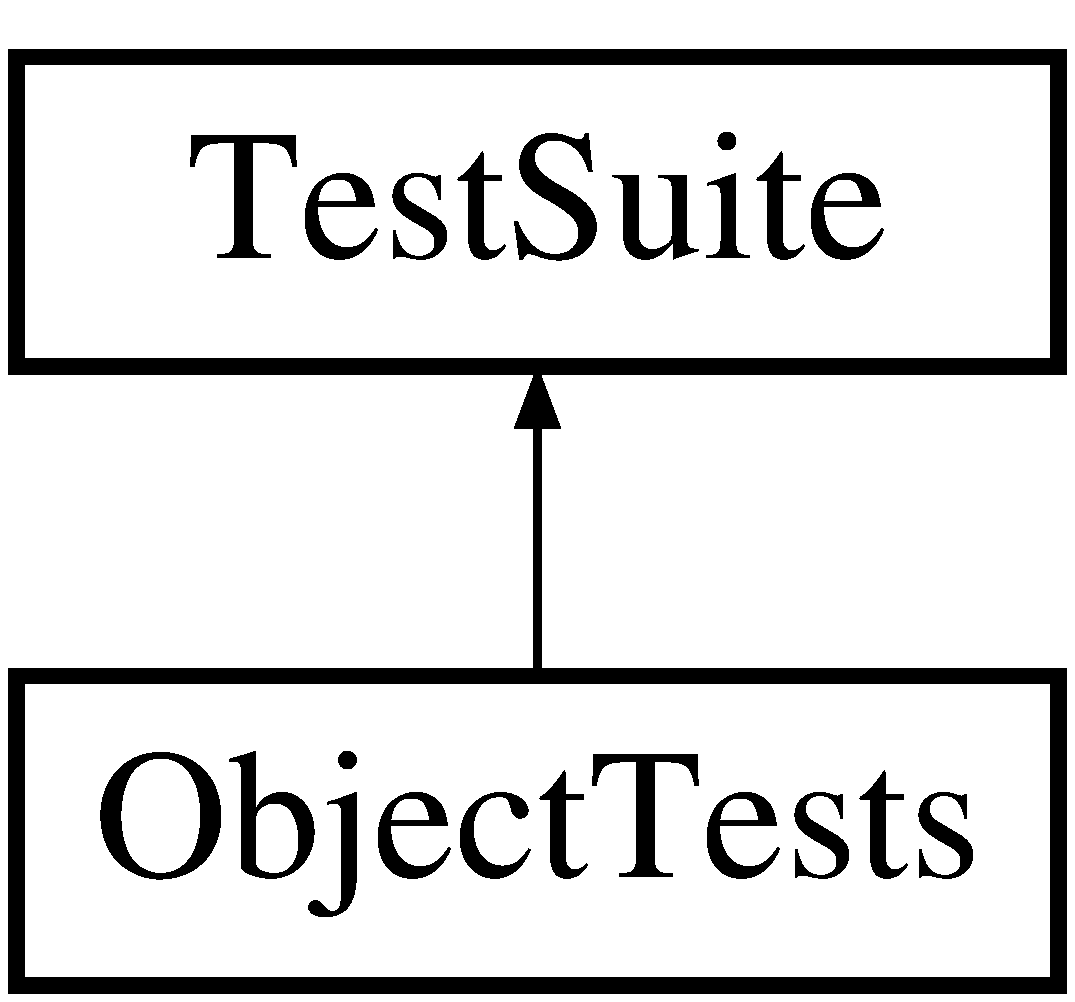
\includegraphics[height=2.000000cm]{classObjectTests}
\end{center}
\end{figure}
\subsection*{Public Member Functions}
\begin{DoxyCompactItemize}
\item 
void \hyperlink{classObjectTests_a85cdff21ccdcde04467372ae3abab902}{Test\-\_\-set\-Shape} (void)
\begin{DoxyCompactList}\small\item\em test whether set\-Shape function works well. \end{DoxyCompactList}\item 
void \hyperlink{classObjectTests_a65ea2e4d100fafec3dae904b4388c30e}{Test\-\_\-move\-Dist} (void)
\begin{DoxyCompactList}\small\item\em test whether move function works well in calculate deltadistance. \end{DoxyCompactList}\item 
void \hyperlink{classObjectTests_a2dbc3484f891810c18b831d326a3fdac}{Test\-\_\-move\-Ori} (void)
\begin{DoxyCompactList}\small\item\em test whether move function works well in calculate delta\-Ori. \end{DoxyCompactList}\item 
void \hyperlink{classObjectTests_a6deb7c9f475754e836f23edd17a11e51}{Test\-\_\-rotate} (void)
\begin{DoxyCompactList}\small\item\em test whether rotate function works well \end{DoxyCompactList}\item 
void \hyperlink{classObjectTests_a47b3e74691b343e097d5e0bbddc2e8c3}{Test\-\_\-set\-Color} (void)
\begin{DoxyCompactList}\small\item\em test whether set\-Color function works well in setting object's color. \end{DoxyCompactList}\item 
void \hyperlink{classObjectTests_ae0fc1474d18ba57a69660ac6e60f27f1}{Test\-\_\-set\-Type} (void)
\begin{DoxyCompactList}\small\item\em test whether set\-Type function works well \end{DoxyCompactList}\item 
void \hyperlink{classObjectTests_a7438b8610b6dc1b8eba65110f596a5d6}{Test\-\_\-set\-X\-Position\-Regular} (void)
\begin{DoxyCompactList}\small\item\em test whether set\-Position function works well in setting robot's X position. \end{DoxyCompactList}\item 
void \hyperlink{classObjectTests_adefdeada43ea50fe1b0334bedc7400c7}{Test\-\_\-set\-Y\-Position\-Regular} (void)
\begin{DoxyCompactList}\small\item\em test whether set\-Position function works well in setting robot's Y position. \end{DoxyCompactList}\item 
void \hyperlink{classObjectTests_a56da3c8ba84487866849205cdc3ca014}{Test\-\_\-set\-X\-Position\-Negetive\-Num} (void)
\begin{DoxyCompactList}\small\item\em test whether set\-Position function works well in setting X position to random value when negative input of X. \end{DoxyCompactList}\item 
void \hyperlink{classObjectTests_a7ccdbab9e0a7fc65c68f962062a6fd0f}{Test\-\_\-set\-Y\-Position\-Negetive\-Num} (void)
\begin{DoxyCompactList}\small\item\em test whether set\-Position function works well in setting Y position to random value when negative input of Y. \end{DoxyCompactList}\item 
void \hyperlink{classObjectTests_acfe64542be015eb777ad8f6e17bfa8c7}{Test\-\_\-set\-X\-Position\-Larger\-Num1} (void)
\begin{DoxyCompactList}\small\item\em test whether set\-Position function works well in setting X position to random value when beyond bounder input of X. \end{DoxyCompactList}\item 
void \hyperlink{classObjectTests_aaee0a0fad26b5bebfce14ff81d2b186c}{Test\-\_\-set\-X\-Position\-Larger\-Num2} (void)
\begin{DoxyCompactList}\small\item\em test whether set\-Position function works well in setting X position to random value when beyond bounder input of X. \end{DoxyCompactList}\item 
void \hyperlink{classObjectTests_a9aabec99604e89967320e7ba85a5be38}{Test\-\_\-set\-Y\-Position\-Larger\-Num1} (void)
\begin{DoxyCompactList}\small\item\em test whether set\-Position function works well in setting Y position to random value when beyond bounder input of Y. \end{DoxyCompactList}\item 
void \hyperlink{classObjectTests_a2db50cd40ae9c013e4dc8de85cd174f8}{Test\-\_\-set\-Y\-Position\-Larger\-Num2} (void)
\begin{DoxyCompactList}\small\item\em test whether set\-Position function works well in setting Y position to random value when beyond bounder input of Y. \end{DoxyCompactList}\item 
void \hyperlink{classObjectTests_a2c24cb7e640edfab1350c7fd6bae30ee}{Test\-\_\-set\-Size\-Regular} (void)
\begin{DoxyCompactList}\small\item\em test whether set\-Size function works well in regular value. \end{DoxyCompactList}\item 
void \hyperlink{classObjectTests_aea19fefb82d85e2354aa36e20001a1ee}{Test\-\_\-set\-Size\-\_\-bigger\-\_\-than\-\_\-60\-\_\-1} (void)
\begin{DoxyCompactList}\small\item\em test whether set\-Size function works well in beyond bounder value. \end{DoxyCompactList}\item 
void \hyperlink{classObjectTests_acb11b07a5ec45e71e5e659b3e7172fe3}{Test\-\_\-set\-Size\-\_\-bigger\-\_\-than\-\_\-60\-\_\-2} (void)
\begin{DoxyCompactList}\small\item\em test whether set\-Size function works well in beyond upper bound value. \end{DoxyCompactList}\item 
void \hyperlink{classObjectTests_a4447d749d95d2d1fe87ba82d30babc78}{Test\-\_\-set\-Size\-\_\-less\-\_\-than\-\_\-20\-\_\-1} (void)
\begin{DoxyCompactList}\small\item\em test whether set\-Size function works well in below lower bound value. \end{DoxyCompactList}\item 
void \hyperlink{classObjectTests_a17b80732faa07515ce308285c243220f}{Test\-\_\-set\-Size\-\_\-less\-\_\-than\-\_\-20\-\_\-2} (void)
\begin{DoxyCompactList}\small\item\em test whether set\-Size function works well in below lower bound value. \end{DoxyCompactList}\item 
void \hyperlink{classObjectTests_af81ace2398dad8139a6c1d25de79de0d}{Test\-\_\-get\-X\-Position} (void)
\begin{DoxyCompactList}\small\item\em test whether get\-X\-Position function works well. \end{DoxyCompactList}\item 
void \hyperlink{classObjectTests_a881750d276c37304b1e28855ec7efd89}{Test\-\_\-get\-Y\-Position} (void)
\begin{DoxyCompactList}\small\item\em test whether get\-X\-Position function works well. \end{DoxyCompactList}\item 
void \hyperlink{classObjectTests_aeb1525bf71b652c62bec9efb0a207683}{Test\-\_\-get\-Size} (void)
\begin{DoxyCompactList}\small\item\em test whether get\-Size function works well. \end{DoxyCompactList}\item 
void \hyperlink{classObjectTests_aa990ea69bf041eb56b9f5eaf77147dd7}{Test\-\_\-set\-Orientation\-\_\-regular} (void)
\begin{DoxyCompactList}\small\item\em test whether set\-Orientation function works well in regular values. \end{DoxyCompactList}\item 
void \hyperlink{classObjectTests_a41f09e4861c008db7a8ccbc269c2e709}{Test\-\_\-set\-Orientation\-\_\-bigger\-\_\-than\-\_\-360\-\_\-1} (void)
\begin{DoxyCompactList}\small\item\em test whether set\-Orientation function works well in beyond upper bound values. \end{DoxyCompactList}\item 
void \hyperlink{classObjectTests_a847dd35383f5542c3d7c96e758bc4898}{Test\-\_\-set\-Orientation\-\_\-bigger\-\_\-than\-\_\-360\-\_\-2} (void)
\begin{DoxyCompactList}\small\item\em test whether set\-Orientation function works well in beyond upper bound values. \end{DoxyCompactList}\item 
void \hyperlink{classObjectTests_aad4c222661558640bb487a7880b5a326}{Test\-\_\-set\-Orientation\-\_\-negative\-\_\-1} (void)
\begin{DoxyCompactList}\small\item\em test whether set\-Orientation function works well in negative values. \end{DoxyCompactList}\item 
void \hyperlink{classObjectTests_a82f42fddbe68538ca457961382109889}{Test\-\_\-set\-Orientation\-\_\-negative\-\_\-2} (void)
\begin{DoxyCompactList}\small\item\em test whether set\-Orientation function works well in negative values. \end{DoxyCompactList}\item 
void \hyperlink{classObjectTests_a7bac3f755703531183355993f8c880cc}{Test\-\_\-set\-Speed} (void)
\begin{DoxyCompactList}\small\item\em test whether set\-Speed function works well in regular values. \end{DoxyCompactList}\item 
void \hyperlink{classObjectTests_a2cf438a435380b1258587c55d652ffc3}{Test\-\_\-set\-Speed\-\_\-\-Negative} (void)
\begin{DoxyCompactList}\small\item\em test whether set\-Speed function works well in negative values. \end{DoxyCompactList}\item 
void \hyperlink{classObjectTests_ae3c9867ca18bf9fa6afa9f92ab4fbac3}{Test\-\_\-get\-Orientation} (void)
\begin{DoxyCompactList}\small\item\em test whether get\-Orientation function works well. \end{DoxyCompactList}\item 
void \hyperlink{classObjectTests_ade778461cf9a7dd289768f151303b956}{Test\-\_\-get\-Speed} (void)
\begin{DoxyCompactList}\small\item\em test whether get\-Speed function works well. \end{DoxyCompactList}\item 
void \hyperlink{classObjectTests_a46b29ddba05b7349987bad6f9c9b4147}{Test\-\_\-get\-Color\-\_\-1} (void)
\begin{DoxyCompactList}\small\item\em test whether get\-Color function works well. \end{DoxyCompactList}\item 
void \hyperlink{classObjectTests_a8fb183a34b9af5aebee5015cebbf245c}{Test\-\_\-get\-Color\-\_\-2} (void)
\begin{DoxyCompactList}\small\item\em test whether get\-Color function works well. \end{DoxyCompactList}\item 
void \hyperlink{classObjectTests_a938c749ad8c04ea2700bdf8b5de1b0fd}{Test\-\_\-get\-Color\-\_\-3} (void)
\begin{DoxyCompactList}\small\item\em test whether get\-Color function works well. \end{DoxyCompactList}\item 
void \hyperlink{classObjectTests_a4cdf6a34f4a1a805a273b979883ab437}{Test\-\_\-get\-Object\-Type} (void)
\begin{DoxyCompactList}\small\item\em test whether get\-Object\-Type function works well. \end{DoxyCompactList}\item 
void \hyperlink{classObjectTests_afa6f53eb63b3d20a0d4ecc8a9135abc8}{Test\-\_\-get\-Shape\-Type} (void)
\begin{DoxyCompactList}\small\item\em test whether get\-Shape\-Type function works well. \end{DoxyCompactList}\item 
void \hyperlink{classObjectTests_a558a178a81767c856e9981ed03367b92}{Test\-\_\-get\-I\-D} (void)
\begin{DoxyCompactList}\small\item\em test whether get\-I\-D function works well. \end{DoxyCompactList}\item 
void \hyperlink{classObjectTests_ae845b006977fa7a33d73e36e77cbc59b}{Test\-\_\-detect\-Wall\-Touch\-\_\-\-Top} (void)
\begin{DoxyCompactList}\small\item\em test whether detect\-Wall function works well in collision with Top wall situation. \end{DoxyCompactList}\item 
void \hyperlink{classObjectTests_a53f3339eefc24d3026f7270d790eaefe}{Test\-\_\-detect\-Wall\-Touch\-\_\-\-Bottom} (void)
\begin{DoxyCompactList}\small\item\em test whether detect\-Wall function works well in collision with Bottom wall situation. \end{DoxyCompactList}\item 
void \hyperlink{classObjectTests_ab1694e1c3b2e7b0754ec29acb9b97837}{Test\-\_\-detect\-Wall\-Touch\-\_\-\-Left} (void)
\begin{DoxyCompactList}\small\item\em test whether detect\-Wall function works well in collision with Left wall situation. \end{DoxyCompactList}\item 
void \hyperlink{classObjectTests_aa4cac76075e2988fa0c81c56a5ea8996}{Test\-\_\-detect\-Wall\-Touch\-\_\-\-Right} (void)
\begin{DoxyCompactList}\small\item\em test whether detect\-Wall function works well in collision with Right wall situation. \end{DoxyCompactList}\item 
void \hyperlink{classObjectTests_a0eeb781ec4b01084388c7b75749a0da0}{Test\-\_\-detect\-Wall\-Out\-\_\-\-Top} (void)
\begin{DoxyCompactList}\small\item\em test whether detect\-Wall function works well in collision with Top wall situation. \end{DoxyCompactList}\item 
void \hyperlink{classObjectTests_acea24c799dff75ee75284bfabe5d4c68}{Test\-\_\-detect\-Wall\-Out\-\_\-\-Bottom} (void)
\begin{DoxyCompactList}\small\item\em test whether detect\-Wall function works well in collision with Bottom wall situation. \end{DoxyCompactList}\item 
void \hyperlink{classObjectTests_a1b04be05c8764c131f102cbb5e6f7b84}{Test\-\_\-detect\-Wall\-Out\-\_\-\-Left} (void)
\begin{DoxyCompactList}\small\item\em test whether detect\-Wall function works well in collision with Left wall situation. \end{DoxyCompactList}\item 
void \hyperlink{classObjectTests_a1c05b1d58719770234f733435e4e9f46}{Test\-\_\-detect\-Wall\-Out\-\_\-\-Right} (void)
\begin{DoxyCompactList}\small\item\em test whether detect\-Wall function works well in collision with Right wall situation. \end{DoxyCompactList}\item 
void \hyperlink{classObjectTests_a713c431caa4e88bf0ac4de61119a0eb5}{Test\-\_\-detect\-Wall\-Within\-\_\-\-Top} (void)
\begin{DoxyCompactList}\small\item\em test whether detect\-Wall function works well in collision with Top wall situation. \end{DoxyCompactList}\item 
void \hyperlink{classObjectTests_afa6b29b259842f8549c69c1adea09a6c}{Test\-\_\-detect\-Wall\-Within\-\_\-\-Bottom} (void)
\begin{DoxyCompactList}\small\item\em test whether detect\-Wall function works well in collision with Bottom wall situation. \end{DoxyCompactList}\item 
void \hyperlink{classObjectTests_a45b83d0a628d43eca08e3b5babe978e7}{Test\-\_\-detect\-Wall\-Within\-\_\-\-Left} (void)
\begin{DoxyCompactList}\small\item\em test whether detect\-Wall function works well in collision with Left wall situation. \end{DoxyCompactList}\item 
void \hyperlink{classObjectTests_a2547f1471a274e1e48d553274d26148c}{Test\-\_\-detect\-Wall\-Within\-\_\-\-Right} (void)
\begin{DoxyCompactList}\small\item\em test whether detect\-Wall function works well in collision with Right wall situation. \end{DoxyCompactList}\item 
void \hyperlink{classObjectTests_a6fd794a9bc7550576305b528de2945ff}{Test\-\_\-detect\-Ostacle\-Touch} (void)
\begin{DoxyCompactList}\small\item\em test whether detect\-Obstacle function works well \end{DoxyCompactList}\item 
void \hyperlink{classObjectTests_a8edeba160a6edf0668132146d63de4ba}{Test\-\_\-detect\-Obstacle\-No\-Col} (void)
\begin{DoxyCompactList}\small\item\em test whether detect\-Obstacle function works well in no collision situation. \end{DoxyCompactList}\item 
void \hyperlink{classObjectTests_a1493e5b4f9715b52c6e40de7955b59ba}{Test\-\_\-detect\-Obstacle\-Col} (void)
\begin{DoxyCompactList}\small\item\em test whether detect\-Obstacle function works well \end{DoxyCompactList}\end{DoxyCompactItemize}


\subsection{Member Function Documentation}
\hypertarget{classObjectTests_a1493e5b4f9715b52c6e40de7955b59ba}{\index{Object\-Tests@{Object\-Tests}!Test\-\_\-detect\-Obstacle\-Col@{Test\-\_\-detect\-Obstacle\-Col}}
\index{Test\-\_\-detect\-Obstacle\-Col@{Test\-\_\-detect\-Obstacle\-Col}!ObjectTests@{Object\-Tests}}
\subsubsection[{Test\-\_\-detect\-Obstacle\-Col}]{\setlength{\rightskip}{0pt plus 5cm}void Object\-Tests\-::\-Test\-\_\-detect\-Obstacle\-Col (
\begin{DoxyParamCaption}
\item[{void}]{}
\end{DoxyParamCaption}
)\hspace{0.3cm}{\ttfamily [inline]}}}\label{classObjectTests_a1493e5b4f9715b52c6e40de7955b59ba}


test whether detect\-Obstacle function works well 

\hypertarget{classObjectTests_a8edeba160a6edf0668132146d63de4ba}{\index{Object\-Tests@{Object\-Tests}!Test\-\_\-detect\-Obstacle\-No\-Col@{Test\-\_\-detect\-Obstacle\-No\-Col}}
\index{Test\-\_\-detect\-Obstacle\-No\-Col@{Test\-\_\-detect\-Obstacle\-No\-Col}!ObjectTests@{Object\-Tests}}
\subsubsection[{Test\-\_\-detect\-Obstacle\-No\-Col}]{\setlength{\rightskip}{0pt plus 5cm}void Object\-Tests\-::\-Test\-\_\-detect\-Obstacle\-No\-Col (
\begin{DoxyParamCaption}
\item[{void}]{}
\end{DoxyParamCaption}
)\hspace{0.3cm}{\ttfamily [inline]}}}\label{classObjectTests_a8edeba160a6edf0668132146d63de4ba}


test whether detect\-Obstacle function works well in no collision situation. 

\hypertarget{classObjectTests_a6fd794a9bc7550576305b528de2945ff}{\index{Object\-Tests@{Object\-Tests}!Test\-\_\-detect\-Ostacle\-Touch@{Test\-\_\-detect\-Ostacle\-Touch}}
\index{Test\-\_\-detect\-Ostacle\-Touch@{Test\-\_\-detect\-Ostacle\-Touch}!ObjectTests@{Object\-Tests}}
\subsubsection[{Test\-\_\-detect\-Ostacle\-Touch}]{\setlength{\rightskip}{0pt plus 5cm}void Object\-Tests\-::\-Test\-\_\-detect\-Ostacle\-Touch (
\begin{DoxyParamCaption}
\item[{void}]{}
\end{DoxyParamCaption}
)\hspace{0.3cm}{\ttfamily [inline]}}}\label{classObjectTests_a6fd794a9bc7550576305b528de2945ff}


test whether detect\-Obstacle function works well 

\hypertarget{classObjectTests_acea24c799dff75ee75284bfabe5d4c68}{\index{Object\-Tests@{Object\-Tests}!Test\-\_\-detect\-Wall\-Out\-\_\-\-Bottom@{Test\-\_\-detect\-Wall\-Out\-\_\-\-Bottom}}
\index{Test\-\_\-detect\-Wall\-Out\-\_\-\-Bottom@{Test\-\_\-detect\-Wall\-Out\-\_\-\-Bottom}!ObjectTests@{Object\-Tests}}
\subsubsection[{Test\-\_\-detect\-Wall\-Out\-\_\-\-Bottom}]{\setlength{\rightskip}{0pt plus 5cm}void Object\-Tests\-::\-Test\-\_\-detect\-Wall\-Out\-\_\-\-Bottom (
\begin{DoxyParamCaption}
\item[{void}]{}
\end{DoxyParamCaption}
)\hspace{0.3cm}{\ttfamily [inline]}}}\label{classObjectTests_acea24c799dff75ee75284bfabe5d4c68}


test whether detect\-Wall function works well in collision with Bottom wall situation. 

\hypertarget{classObjectTests_a1b04be05c8764c131f102cbb5e6f7b84}{\index{Object\-Tests@{Object\-Tests}!Test\-\_\-detect\-Wall\-Out\-\_\-\-Left@{Test\-\_\-detect\-Wall\-Out\-\_\-\-Left}}
\index{Test\-\_\-detect\-Wall\-Out\-\_\-\-Left@{Test\-\_\-detect\-Wall\-Out\-\_\-\-Left}!ObjectTests@{Object\-Tests}}
\subsubsection[{Test\-\_\-detect\-Wall\-Out\-\_\-\-Left}]{\setlength{\rightskip}{0pt plus 5cm}void Object\-Tests\-::\-Test\-\_\-detect\-Wall\-Out\-\_\-\-Left (
\begin{DoxyParamCaption}
\item[{void}]{}
\end{DoxyParamCaption}
)\hspace{0.3cm}{\ttfamily [inline]}}}\label{classObjectTests_a1b04be05c8764c131f102cbb5e6f7b84}


test whether detect\-Wall function works well in collision with Left wall situation. 

\hypertarget{classObjectTests_a1c05b1d58719770234f733435e4e9f46}{\index{Object\-Tests@{Object\-Tests}!Test\-\_\-detect\-Wall\-Out\-\_\-\-Right@{Test\-\_\-detect\-Wall\-Out\-\_\-\-Right}}
\index{Test\-\_\-detect\-Wall\-Out\-\_\-\-Right@{Test\-\_\-detect\-Wall\-Out\-\_\-\-Right}!ObjectTests@{Object\-Tests}}
\subsubsection[{Test\-\_\-detect\-Wall\-Out\-\_\-\-Right}]{\setlength{\rightskip}{0pt plus 5cm}void Object\-Tests\-::\-Test\-\_\-detect\-Wall\-Out\-\_\-\-Right (
\begin{DoxyParamCaption}
\item[{void}]{}
\end{DoxyParamCaption}
)\hspace{0.3cm}{\ttfamily [inline]}}}\label{classObjectTests_a1c05b1d58719770234f733435e4e9f46}


test whether detect\-Wall function works well in collision with Right wall situation. 

\hypertarget{classObjectTests_a0eeb781ec4b01084388c7b75749a0da0}{\index{Object\-Tests@{Object\-Tests}!Test\-\_\-detect\-Wall\-Out\-\_\-\-Top@{Test\-\_\-detect\-Wall\-Out\-\_\-\-Top}}
\index{Test\-\_\-detect\-Wall\-Out\-\_\-\-Top@{Test\-\_\-detect\-Wall\-Out\-\_\-\-Top}!ObjectTests@{Object\-Tests}}
\subsubsection[{Test\-\_\-detect\-Wall\-Out\-\_\-\-Top}]{\setlength{\rightskip}{0pt plus 5cm}void Object\-Tests\-::\-Test\-\_\-detect\-Wall\-Out\-\_\-\-Top (
\begin{DoxyParamCaption}
\item[{void}]{}
\end{DoxyParamCaption}
)\hspace{0.3cm}{\ttfamily [inline]}}}\label{classObjectTests_a0eeb781ec4b01084388c7b75749a0da0}


test whether detect\-Wall function works well in collision with Top wall situation. 

\hypertarget{classObjectTests_a53f3339eefc24d3026f7270d790eaefe}{\index{Object\-Tests@{Object\-Tests}!Test\-\_\-detect\-Wall\-Touch\-\_\-\-Bottom@{Test\-\_\-detect\-Wall\-Touch\-\_\-\-Bottom}}
\index{Test\-\_\-detect\-Wall\-Touch\-\_\-\-Bottom@{Test\-\_\-detect\-Wall\-Touch\-\_\-\-Bottom}!ObjectTests@{Object\-Tests}}
\subsubsection[{Test\-\_\-detect\-Wall\-Touch\-\_\-\-Bottom}]{\setlength{\rightskip}{0pt plus 5cm}void Object\-Tests\-::\-Test\-\_\-detect\-Wall\-Touch\-\_\-\-Bottom (
\begin{DoxyParamCaption}
\item[{void}]{}
\end{DoxyParamCaption}
)\hspace{0.3cm}{\ttfamily [inline]}}}\label{classObjectTests_a53f3339eefc24d3026f7270d790eaefe}


test whether detect\-Wall function works well in collision with Bottom wall situation. 

\hypertarget{classObjectTests_ab1694e1c3b2e7b0754ec29acb9b97837}{\index{Object\-Tests@{Object\-Tests}!Test\-\_\-detect\-Wall\-Touch\-\_\-\-Left@{Test\-\_\-detect\-Wall\-Touch\-\_\-\-Left}}
\index{Test\-\_\-detect\-Wall\-Touch\-\_\-\-Left@{Test\-\_\-detect\-Wall\-Touch\-\_\-\-Left}!ObjectTests@{Object\-Tests}}
\subsubsection[{Test\-\_\-detect\-Wall\-Touch\-\_\-\-Left}]{\setlength{\rightskip}{0pt plus 5cm}void Object\-Tests\-::\-Test\-\_\-detect\-Wall\-Touch\-\_\-\-Left (
\begin{DoxyParamCaption}
\item[{void}]{}
\end{DoxyParamCaption}
)\hspace{0.3cm}{\ttfamily [inline]}}}\label{classObjectTests_ab1694e1c3b2e7b0754ec29acb9b97837}


test whether detect\-Wall function works well in collision with Left wall situation. 

\hypertarget{classObjectTests_aa4cac76075e2988fa0c81c56a5ea8996}{\index{Object\-Tests@{Object\-Tests}!Test\-\_\-detect\-Wall\-Touch\-\_\-\-Right@{Test\-\_\-detect\-Wall\-Touch\-\_\-\-Right}}
\index{Test\-\_\-detect\-Wall\-Touch\-\_\-\-Right@{Test\-\_\-detect\-Wall\-Touch\-\_\-\-Right}!ObjectTests@{Object\-Tests}}
\subsubsection[{Test\-\_\-detect\-Wall\-Touch\-\_\-\-Right}]{\setlength{\rightskip}{0pt plus 5cm}void Object\-Tests\-::\-Test\-\_\-detect\-Wall\-Touch\-\_\-\-Right (
\begin{DoxyParamCaption}
\item[{void}]{}
\end{DoxyParamCaption}
)\hspace{0.3cm}{\ttfamily [inline]}}}\label{classObjectTests_aa4cac76075e2988fa0c81c56a5ea8996}


test whether detect\-Wall function works well in collision with Right wall situation. 

\hypertarget{classObjectTests_ae845b006977fa7a33d73e36e77cbc59b}{\index{Object\-Tests@{Object\-Tests}!Test\-\_\-detect\-Wall\-Touch\-\_\-\-Top@{Test\-\_\-detect\-Wall\-Touch\-\_\-\-Top}}
\index{Test\-\_\-detect\-Wall\-Touch\-\_\-\-Top@{Test\-\_\-detect\-Wall\-Touch\-\_\-\-Top}!ObjectTests@{Object\-Tests}}
\subsubsection[{Test\-\_\-detect\-Wall\-Touch\-\_\-\-Top}]{\setlength{\rightskip}{0pt plus 5cm}void Object\-Tests\-::\-Test\-\_\-detect\-Wall\-Touch\-\_\-\-Top (
\begin{DoxyParamCaption}
\item[{void}]{}
\end{DoxyParamCaption}
)\hspace{0.3cm}{\ttfamily [inline]}}}\label{classObjectTests_ae845b006977fa7a33d73e36e77cbc59b}


test whether detect\-Wall function works well in collision with Top wall situation. 

\hypertarget{classObjectTests_afa6b29b259842f8549c69c1adea09a6c}{\index{Object\-Tests@{Object\-Tests}!Test\-\_\-detect\-Wall\-Within\-\_\-\-Bottom@{Test\-\_\-detect\-Wall\-Within\-\_\-\-Bottom}}
\index{Test\-\_\-detect\-Wall\-Within\-\_\-\-Bottom@{Test\-\_\-detect\-Wall\-Within\-\_\-\-Bottom}!ObjectTests@{Object\-Tests}}
\subsubsection[{Test\-\_\-detect\-Wall\-Within\-\_\-\-Bottom}]{\setlength{\rightskip}{0pt plus 5cm}void Object\-Tests\-::\-Test\-\_\-detect\-Wall\-Within\-\_\-\-Bottom (
\begin{DoxyParamCaption}
\item[{void}]{}
\end{DoxyParamCaption}
)\hspace{0.3cm}{\ttfamily [inline]}}}\label{classObjectTests_afa6b29b259842f8549c69c1adea09a6c}


test whether detect\-Wall function works well in collision with Bottom wall situation. 

\hypertarget{classObjectTests_a45b83d0a628d43eca08e3b5babe978e7}{\index{Object\-Tests@{Object\-Tests}!Test\-\_\-detect\-Wall\-Within\-\_\-\-Left@{Test\-\_\-detect\-Wall\-Within\-\_\-\-Left}}
\index{Test\-\_\-detect\-Wall\-Within\-\_\-\-Left@{Test\-\_\-detect\-Wall\-Within\-\_\-\-Left}!ObjectTests@{Object\-Tests}}
\subsubsection[{Test\-\_\-detect\-Wall\-Within\-\_\-\-Left}]{\setlength{\rightskip}{0pt plus 5cm}void Object\-Tests\-::\-Test\-\_\-detect\-Wall\-Within\-\_\-\-Left (
\begin{DoxyParamCaption}
\item[{void}]{}
\end{DoxyParamCaption}
)\hspace{0.3cm}{\ttfamily [inline]}}}\label{classObjectTests_a45b83d0a628d43eca08e3b5babe978e7}


test whether detect\-Wall function works well in collision with Left wall situation. 

\hypertarget{classObjectTests_a2547f1471a274e1e48d553274d26148c}{\index{Object\-Tests@{Object\-Tests}!Test\-\_\-detect\-Wall\-Within\-\_\-\-Right@{Test\-\_\-detect\-Wall\-Within\-\_\-\-Right}}
\index{Test\-\_\-detect\-Wall\-Within\-\_\-\-Right@{Test\-\_\-detect\-Wall\-Within\-\_\-\-Right}!ObjectTests@{Object\-Tests}}
\subsubsection[{Test\-\_\-detect\-Wall\-Within\-\_\-\-Right}]{\setlength{\rightskip}{0pt plus 5cm}void Object\-Tests\-::\-Test\-\_\-detect\-Wall\-Within\-\_\-\-Right (
\begin{DoxyParamCaption}
\item[{void}]{}
\end{DoxyParamCaption}
)\hspace{0.3cm}{\ttfamily [inline]}}}\label{classObjectTests_a2547f1471a274e1e48d553274d26148c}


test whether detect\-Wall function works well in collision with Right wall situation. 

\hypertarget{classObjectTests_a713c431caa4e88bf0ac4de61119a0eb5}{\index{Object\-Tests@{Object\-Tests}!Test\-\_\-detect\-Wall\-Within\-\_\-\-Top@{Test\-\_\-detect\-Wall\-Within\-\_\-\-Top}}
\index{Test\-\_\-detect\-Wall\-Within\-\_\-\-Top@{Test\-\_\-detect\-Wall\-Within\-\_\-\-Top}!ObjectTests@{Object\-Tests}}
\subsubsection[{Test\-\_\-detect\-Wall\-Within\-\_\-\-Top}]{\setlength{\rightskip}{0pt plus 5cm}void Object\-Tests\-::\-Test\-\_\-detect\-Wall\-Within\-\_\-\-Top (
\begin{DoxyParamCaption}
\item[{void}]{}
\end{DoxyParamCaption}
)\hspace{0.3cm}{\ttfamily [inline]}}}\label{classObjectTests_a713c431caa4e88bf0ac4de61119a0eb5}


test whether detect\-Wall function works well in collision with Top wall situation. 

\hypertarget{classObjectTests_a46b29ddba05b7349987bad6f9c9b4147}{\index{Object\-Tests@{Object\-Tests}!Test\-\_\-get\-Color\-\_\-1@{Test\-\_\-get\-Color\-\_\-1}}
\index{Test\-\_\-get\-Color\-\_\-1@{Test\-\_\-get\-Color\-\_\-1}!ObjectTests@{Object\-Tests}}
\subsubsection[{Test\-\_\-get\-Color\-\_\-1}]{\setlength{\rightskip}{0pt plus 5cm}void Object\-Tests\-::\-Test\-\_\-get\-Color\-\_\-1 (
\begin{DoxyParamCaption}
\item[{void}]{}
\end{DoxyParamCaption}
)\hspace{0.3cm}{\ttfamily [inline]}}}\label{classObjectTests_a46b29ddba05b7349987bad6f9c9b4147}


test whether get\-Color function works well. 

\hypertarget{classObjectTests_a8fb183a34b9af5aebee5015cebbf245c}{\index{Object\-Tests@{Object\-Tests}!Test\-\_\-get\-Color\-\_\-2@{Test\-\_\-get\-Color\-\_\-2}}
\index{Test\-\_\-get\-Color\-\_\-2@{Test\-\_\-get\-Color\-\_\-2}!ObjectTests@{Object\-Tests}}
\subsubsection[{Test\-\_\-get\-Color\-\_\-2}]{\setlength{\rightskip}{0pt plus 5cm}void Object\-Tests\-::\-Test\-\_\-get\-Color\-\_\-2 (
\begin{DoxyParamCaption}
\item[{void}]{}
\end{DoxyParamCaption}
)\hspace{0.3cm}{\ttfamily [inline]}}}\label{classObjectTests_a8fb183a34b9af5aebee5015cebbf245c}


test whether get\-Color function works well. 

\hypertarget{classObjectTests_a938c749ad8c04ea2700bdf8b5de1b0fd}{\index{Object\-Tests@{Object\-Tests}!Test\-\_\-get\-Color\-\_\-3@{Test\-\_\-get\-Color\-\_\-3}}
\index{Test\-\_\-get\-Color\-\_\-3@{Test\-\_\-get\-Color\-\_\-3}!ObjectTests@{Object\-Tests}}
\subsubsection[{Test\-\_\-get\-Color\-\_\-3}]{\setlength{\rightskip}{0pt plus 5cm}void Object\-Tests\-::\-Test\-\_\-get\-Color\-\_\-3 (
\begin{DoxyParamCaption}
\item[{void}]{}
\end{DoxyParamCaption}
)\hspace{0.3cm}{\ttfamily [inline]}}}\label{classObjectTests_a938c749ad8c04ea2700bdf8b5de1b0fd}


test whether get\-Color function works well. 

\hypertarget{classObjectTests_a558a178a81767c856e9981ed03367b92}{\index{Object\-Tests@{Object\-Tests}!Test\-\_\-get\-I\-D@{Test\-\_\-get\-I\-D}}
\index{Test\-\_\-get\-I\-D@{Test\-\_\-get\-I\-D}!ObjectTests@{Object\-Tests}}
\subsubsection[{Test\-\_\-get\-I\-D}]{\setlength{\rightskip}{0pt plus 5cm}void Object\-Tests\-::\-Test\-\_\-get\-I\-D (
\begin{DoxyParamCaption}
\item[{void}]{}
\end{DoxyParamCaption}
)\hspace{0.3cm}{\ttfamily [inline]}}}\label{classObjectTests_a558a178a81767c856e9981ed03367b92}


test whether get\-I\-D function works well. 

\hypertarget{classObjectTests_a4cdf6a34f4a1a805a273b979883ab437}{\index{Object\-Tests@{Object\-Tests}!Test\-\_\-get\-Object\-Type@{Test\-\_\-get\-Object\-Type}}
\index{Test\-\_\-get\-Object\-Type@{Test\-\_\-get\-Object\-Type}!ObjectTests@{Object\-Tests}}
\subsubsection[{Test\-\_\-get\-Object\-Type}]{\setlength{\rightskip}{0pt plus 5cm}void Object\-Tests\-::\-Test\-\_\-get\-Object\-Type (
\begin{DoxyParamCaption}
\item[{void}]{}
\end{DoxyParamCaption}
)\hspace{0.3cm}{\ttfamily [inline]}}}\label{classObjectTests_a4cdf6a34f4a1a805a273b979883ab437}


test whether get\-Object\-Type function works well. 

\hypertarget{classObjectTests_ae3c9867ca18bf9fa6afa9f92ab4fbac3}{\index{Object\-Tests@{Object\-Tests}!Test\-\_\-get\-Orientation@{Test\-\_\-get\-Orientation}}
\index{Test\-\_\-get\-Orientation@{Test\-\_\-get\-Orientation}!ObjectTests@{Object\-Tests}}
\subsubsection[{Test\-\_\-get\-Orientation}]{\setlength{\rightskip}{0pt plus 5cm}void Object\-Tests\-::\-Test\-\_\-get\-Orientation (
\begin{DoxyParamCaption}
\item[{void}]{}
\end{DoxyParamCaption}
)\hspace{0.3cm}{\ttfamily [inline]}}}\label{classObjectTests_ae3c9867ca18bf9fa6afa9f92ab4fbac3}


test whether get\-Orientation function works well. 

\hypertarget{classObjectTests_afa6f53eb63b3d20a0d4ecc8a9135abc8}{\index{Object\-Tests@{Object\-Tests}!Test\-\_\-get\-Shape\-Type@{Test\-\_\-get\-Shape\-Type}}
\index{Test\-\_\-get\-Shape\-Type@{Test\-\_\-get\-Shape\-Type}!ObjectTests@{Object\-Tests}}
\subsubsection[{Test\-\_\-get\-Shape\-Type}]{\setlength{\rightskip}{0pt plus 5cm}void Object\-Tests\-::\-Test\-\_\-get\-Shape\-Type (
\begin{DoxyParamCaption}
\item[{void}]{}
\end{DoxyParamCaption}
)\hspace{0.3cm}{\ttfamily [inline]}}}\label{classObjectTests_afa6f53eb63b3d20a0d4ecc8a9135abc8}


test whether get\-Shape\-Type function works well. 

\hypertarget{classObjectTests_aeb1525bf71b652c62bec9efb0a207683}{\index{Object\-Tests@{Object\-Tests}!Test\-\_\-get\-Size@{Test\-\_\-get\-Size}}
\index{Test\-\_\-get\-Size@{Test\-\_\-get\-Size}!ObjectTests@{Object\-Tests}}
\subsubsection[{Test\-\_\-get\-Size}]{\setlength{\rightskip}{0pt plus 5cm}void Object\-Tests\-::\-Test\-\_\-get\-Size (
\begin{DoxyParamCaption}
\item[{void}]{}
\end{DoxyParamCaption}
)\hspace{0.3cm}{\ttfamily [inline]}}}\label{classObjectTests_aeb1525bf71b652c62bec9efb0a207683}


test whether get\-Size function works well. 

\hypertarget{classObjectTests_ade778461cf9a7dd289768f151303b956}{\index{Object\-Tests@{Object\-Tests}!Test\-\_\-get\-Speed@{Test\-\_\-get\-Speed}}
\index{Test\-\_\-get\-Speed@{Test\-\_\-get\-Speed}!ObjectTests@{Object\-Tests}}
\subsubsection[{Test\-\_\-get\-Speed}]{\setlength{\rightskip}{0pt plus 5cm}void Object\-Tests\-::\-Test\-\_\-get\-Speed (
\begin{DoxyParamCaption}
\item[{void}]{}
\end{DoxyParamCaption}
)\hspace{0.3cm}{\ttfamily [inline]}}}\label{classObjectTests_ade778461cf9a7dd289768f151303b956}


test whether get\-Speed function works well. 

\hypertarget{classObjectTests_af81ace2398dad8139a6c1d25de79de0d}{\index{Object\-Tests@{Object\-Tests}!Test\-\_\-get\-X\-Position@{Test\-\_\-get\-X\-Position}}
\index{Test\-\_\-get\-X\-Position@{Test\-\_\-get\-X\-Position}!ObjectTests@{Object\-Tests}}
\subsubsection[{Test\-\_\-get\-X\-Position}]{\setlength{\rightskip}{0pt plus 5cm}void Object\-Tests\-::\-Test\-\_\-get\-X\-Position (
\begin{DoxyParamCaption}
\item[{void}]{}
\end{DoxyParamCaption}
)\hspace{0.3cm}{\ttfamily [inline]}}}\label{classObjectTests_af81ace2398dad8139a6c1d25de79de0d}


test whether get\-X\-Position function works well. 

\hypertarget{classObjectTests_a881750d276c37304b1e28855ec7efd89}{\index{Object\-Tests@{Object\-Tests}!Test\-\_\-get\-Y\-Position@{Test\-\_\-get\-Y\-Position}}
\index{Test\-\_\-get\-Y\-Position@{Test\-\_\-get\-Y\-Position}!ObjectTests@{Object\-Tests}}
\subsubsection[{Test\-\_\-get\-Y\-Position}]{\setlength{\rightskip}{0pt plus 5cm}void Object\-Tests\-::\-Test\-\_\-get\-Y\-Position (
\begin{DoxyParamCaption}
\item[{void}]{}
\end{DoxyParamCaption}
)\hspace{0.3cm}{\ttfamily [inline]}}}\label{classObjectTests_a881750d276c37304b1e28855ec7efd89}


test whether get\-X\-Position function works well. 

\hypertarget{classObjectTests_a65ea2e4d100fafec3dae904b4388c30e}{\index{Object\-Tests@{Object\-Tests}!Test\-\_\-move\-Dist@{Test\-\_\-move\-Dist}}
\index{Test\-\_\-move\-Dist@{Test\-\_\-move\-Dist}!ObjectTests@{Object\-Tests}}
\subsubsection[{Test\-\_\-move\-Dist}]{\setlength{\rightskip}{0pt plus 5cm}void Object\-Tests\-::\-Test\-\_\-move\-Dist (
\begin{DoxyParamCaption}
\item[{void}]{}
\end{DoxyParamCaption}
)\hspace{0.3cm}{\ttfamily [inline]}}}\label{classObjectTests_a65ea2e4d100fafec3dae904b4388c30e}


test whether move function works well in calculate deltadistance. 

\hypertarget{classObjectTests_a2dbc3484f891810c18b831d326a3fdac}{\index{Object\-Tests@{Object\-Tests}!Test\-\_\-move\-Ori@{Test\-\_\-move\-Ori}}
\index{Test\-\_\-move\-Ori@{Test\-\_\-move\-Ori}!ObjectTests@{Object\-Tests}}
\subsubsection[{Test\-\_\-move\-Ori}]{\setlength{\rightskip}{0pt plus 5cm}void Object\-Tests\-::\-Test\-\_\-move\-Ori (
\begin{DoxyParamCaption}
\item[{void}]{}
\end{DoxyParamCaption}
)\hspace{0.3cm}{\ttfamily [inline]}}}\label{classObjectTests_a2dbc3484f891810c18b831d326a3fdac}


test whether move function works well in calculate delta\-Ori. 

\hypertarget{classObjectTests_a6deb7c9f475754e836f23edd17a11e51}{\index{Object\-Tests@{Object\-Tests}!Test\-\_\-rotate@{Test\-\_\-rotate}}
\index{Test\-\_\-rotate@{Test\-\_\-rotate}!ObjectTests@{Object\-Tests}}
\subsubsection[{Test\-\_\-rotate}]{\setlength{\rightskip}{0pt plus 5cm}void Object\-Tests\-::\-Test\-\_\-rotate (
\begin{DoxyParamCaption}
\item[{void}]{}
\end{DoxyParamCaption}
)\hspace{0.3cm}{\ttfamily [inline]}}}\label{classObjectTests_a6deb7c9f475754e836f23edd17a11e51}


test whether rotate function works well 

\hypertarget{classObjectTests_a47b3e74691b343e097d5e0bbddc2e8c3}{\index{Object\-Tests@{Object\-Tests}!Test\-\_\-set\-Color@{Test\-\_\-set\-Color}}
\index{Test\-\_\-set\-Color@{Test\-\_\-set\-Color}!ObjectTests@{Object\-Tests}}
\subsubsection[{Test\-\_\-set\-Color}]{\setlength{\rightskip}{0pt plus 5cm}void Object\-Tests\-::\-Test\-\_\-set\-Color (
\begin{DoxyParamCaption}
\item[{void}]{}
\end{DoxyParamCaption}
)\hspace{0.3cm}{\ttfamily [inline]}}}\label{classObjectTests_a47b3e74691b343e097d5e0bbddc2e8c3}


test whether set\-Color function works well in setting object's color. 

\hypertarget{classObjectTests_a41f09e4861c008db7a8ccbc269c2e709}{\index{Object\-Tests@{Object\-Tests}!Test\-\_\-set\-Orientation\-\_\-bigger\-\_\-than\-\_\-360\-\_\-1@{Test\-\_\-set\-Orientation\-\_\-bigger\-\_\-than\-\_\-360\-\_\-1}}
\index{Test\-\_\-set\-Orientation\-\_\-bigger\-\_\-than\-\_\-360\-\_\-1@{Test\-\_\-set\-Orientation\-\_\-bigger\-\_\-than\-\_\-360\-\_\-1}!ObjectTests@{Object\-Tests}}
\subsubsection[{Test\-\_\-set\-Orientation\-\_\-bigger\-\_\-than\-\_\-360\-\_\-1}]{\setlength{\rightskip}{0pt plus 5cm}void Object\-Tests\-::\-Test\-\_\-set\-Orientation\-\_\-bigger\-\_\-than\-\_\-360\-\_\-1 (
\begin{DoxyParamCaption}
\item[{void}]{}
\end{DoxyParamCaption}
)\hspace{0.3cm}{\ttfamily [inline]}}}\label{classObjectTests_a41f09e4861c008db7a8ccbc269c2e709}


test whether set\-Orientation function works well in beyond upper bound values. 

\hypertarget{classObjectTests_a847dd35383f5542c3d7c96e758bc4898}{\index{Object\-Tests@{Object\-Tests}!Test\-\_\-set\-Orientation\-\_\-bigger\-\_\-than\-\_\-360\-\_\-2@{Test\-\_\-set\-Orientation\-\_\-bigger\-\_\-than\-\_\-360\-\_\-2}}
\index{Test\-\_\-set\-Orientation\-\_\-bigger\-\_\-than\-\_\-360\-\_\-2@{Test\-\_\-set\-Orientation\-\_\-bigger\-\_\-than\-\_\-360\-\_\-2}!ObjectTests@{Object\-Tests}}
\subsubsection[{Test\-\_\-set\-Orientation\-\_\-bigger\-\_\-than\-\_\-360\-\_\-2}]{\setlength{\rightskip}{0pt plus 5cm}void Object\-Tests\-::\-Test\-\_\-set\-Orientation\-\_\-bigger\-\_\-than\-\_\-360\-\_\-2 (
\begin{DoxyParamCaption}
\item[{void}]{}
\end{DoxyParamCaption}
)\hspace{0.3cm}{\ttfamily [inline]}}}\label{classObjectTests_a847dd35383f5542c3d7c96e758bc4898}


test whether set\-Orientation function works well in beyond upper bound values. 

\hypertarget{classObjectTests_aad4c222661558640bb487a7880b5a326}{\index{Object\-Tests@{Object\-Tests}!Test\-\_\-set\-Orientation\-\_\-negative\-\_\-1@{Test\-\_\-set\-Orientation\-\_\-negative\-\_\-1}}
\index{Test\-\_\-set\-Orientation\-\_\-negative\-\_\-1@{Test\-\_\-set\-Orientation\-\_\-negative\-\_\-1}!ObjectTests@{Object\-Tests}}
\subsubsection[{Test\-\_\-set\-Orientation\-\_\-negative\-\_\-1}]{\setlength{\rightskip}{0pt plus 5cm}void Object\-Tests\-::\-Test\-\_\-set\-Orientation\-\_\-negative\-\_\-1 (
\begin{DoxyParamCaption}
\item[{void}]{}
\end{DoxyParamCaption}
)\hspace{0.3cm}{\ttfamily [inline]}}}\label{classObjectTests_aad4c222661558640bb487a7880b5a326}


test whether set\-Orientation function works well in negative values. 

\hypertarget{classObjectTests_a82f42fddbe68538ca457961382109889}{\index{Object\-Tests@{Object\-Tests}!Test\-\_\-set\-Orientation\-\_\-negative\-\_\-2@{Test\-\_\-set\-Orientation\-\_\-negative\-\_\-2}}
\index{Test\-\_\-set\-Orientation\-\_\-negative\-\_\-2@{Test\-\_\-set\-Orientation\-\_\-negative\-\_\-2}!ObjectTests@{Object\-Tests}}
\subsubsection[{Test\-\_\-set\-Orientation\-\_\-negative\-\_\-2}]{\setlength{\rightskip}{0pt plus 5cm}void Object\-Tests\-::\-Test\-\_\-set\-Orientation\-\_\-negative\-\_\-2 (
\begin{DoxyParamCaption}
\item[{void}]{}
\end{DoxyParamCaption}
)\hspace{0.3cm}{\ttfamily [inline]}}}\label{classObjectTests_a82f42fddbe68538ca457961382109889}


test whether set\-Orientation function works well in negative values. 

\hypertarget{classObjectTests_aa990ea69bf041eb56b9f5eaf77147dd7}{\index{Object\-Tests@{Object\-Tests}!Test\-\_\-set\-Orientation\-\_\-regular@{Test\-\_\-set\-Orientation\-\_\-regular}}
\index{Test\-\_\-set\-Orientation\-\_\-regular@{Test\-\_\-set\-Orientation\-\_\-regular}!ObjectTests@{Object\-Tests}}
\subsubsection[{Test\-\_\-set\-Orientation\-\_\-regular}]{\setlength{\rightskip}{0pt plus 5cm}void Object\-Tests\-::\-Test\-\_\-set\-Orientation\-\_\-regular (
\begin{DoxyParamCaption}
\item[{void}]{}
\end{DoxyParamCaption}
)\hspace{0.3cm}{\ttfamily [inline]}}}\label{classObjectTests_aa990ea69bf041eb56b9f5eaf77147dd7}


test whether set\-Orientation function works well in regular values. 

\hypertarget{classObjectTests_a85cdff21ccdcde04467372ae3abab902}{\index{Object\-Tests@{Object\-Tests}!Test\-\_\-set\-Shape@{Test\-\_\-set\-Shape}}
\index{Test\-\_\-set\-Shape@{Test\-\_\-set\-Shape}!ObjectTests@{Object\-Tests}}
\subsubsection[{Test\-\_\-set\-Shape}]{\setlength{\rightskip}{0pt plus 5cm}void Object\-Tests\-::\-Test\-\_\-set\-Shape (
\begin{DoxyParamCaption}
\item[{void}]{}
\end{DoxyParamCaption}
)\hspace{0.3cm}{\ttfamily [inline]}}}\label{classObjectTests_a85cdff21ccdcde04467372ae3abab902}


test whether set\-Shape function works well. 

\hypertarget{classObjectTests_aea19fefb82d85e2354aa36e20001a1ee}{\index{Object\-Tests@{Object\-Tests}!Test\-\_\-set\-Size\-\_\-bigger\-\_\-than\-\_\-60\-\_\-1@{Test\-\_\-set\-Size\-\_\-bigger\-\_\-than\-\_\-60\-\_\-1}}
\index{Test\-\_\-set\-Size\-\_\-bigger\-\_\-than\-\_\-60\-\_\-1@{Test\-\_\-set\-Size\-\_\-bigger\-\_\-than\-\_\-60\-\_\-1}!ObjectTests@{Object\-Tests}}
\subsubsection[{Test\-\_\-set\-Size\-\_\-bigger\-\_\-than\-\_\-60\-\_\-1}]{\setlength{\rightskip}{0pt plus 5cm}void Object\-Tests\-::\-Test\-\_\-set\-Size\-\_\-bigger\-\_\-than\-\_\-60\-\_\-1 (
\begin{DoxyParamCaption}
\item[{void}]{}
\end{DoxyParamCaption}
)\hspace{0.3cm}{\ttfamily [inline]}}}\label{classObjectTests_aea19fefb82d85e2354aa36e20001a1ee}


test whether set\-Size function works well in beyond bounder value. 

\hypertarget{classObjectTests_acb11b07a5ec45e71e5e659b3e7172fe3}{\index{Object\-Tests@{Object\-Tests}!Test\-\_\-set\-Size\-\_\-bigger\-\_\-than\-\_\-60\-\_\-2@{Test\-\_\-set\-Size\-\_\-bigger\-\_\-than\-\_\-60\-\_\-2}}
\index{Test\-\_\-set\-Size\-\_\-bigger\-\_\-than\-\_\-60\-\_\-2@{Test\-\_\-set\-Size\-\_\-bigger\-\_\-than\-\_\-60\-\_\-2}!ObjectTests@{Object\-Tests}}
\subsubsection[{Test\-\_\-set\-Size\-\_\-bigger\-\_\-than\-\_\-60\-\_\-2}]{\setlength{\rightskip}{0pt plus 5cm}void Object\-Tests\-::\-Test\-\_\-set\-Size\-\_\-bigger\-\_\-than\-\_\-60\-\_\-2 (
\begin{DoxyParamCaption}
\item[{void}]{}
\end{DoxyParamCaption}
)\hspace{0.3cm}{\ttfamily [inline]}}}\label{classObjectTests_acb11b07a5ec45e71e5e659b3e7172fe3}


test whether set\-Size function works well in beyond upper bound value. 

\hypertarget{classObjectTests_a4447d749d95d2d1fe87ba82d30babc78}{\index{Object\-Tests@{Object\-Tests}!Test\-\_\-set\-Size\-\_\-less\-\_\-than\-\_\-20\-\_\-1@{Test\-\_\-set\-Size\-\_\-less\-\_\-than\-\_\-20\-\_\-1}}
\index{Test\-\_\-set\-Size\-\_\-less\-\_\-than\-\_\-20\-\_\-1@{Test\-\_\-set\-Size\-\_\-less\-\_\-than\-\_\-20\-\_\-1}!ObjectTests@{Object\-Tests}}
\subsubsection[{Test\-\_\-set\-Size\-\_\-less\-\_\-than\-\_\-20\-\_\-1}]{\setlength{\rightskip}{0pt plus 5cm}void Object\-Tests\-::\-Test\-\_\-set\-Size\-\_\-less\-\_\-than\-\_\-20\-\_\-1 (
\begin{DoxyParamCaption}
\item[{void}]{}
\end{DoxyParamCaption}
)\hspace{0.3cm}{\ttfamily [inline]}}}\label{classObjectTests_a4447d749d95d2d1fe87ba82d30babc78}


test whether set\-Size function works well in below lower bound value. 

\hypertarget{classObjectTests_a17b80732faa07515ce308285c243220f}{\index{Object\-Tests@{Object\-Tests}!Test\-\_\-set\-Size\-\_\-less\-\_\-than\-\_\-20\-\_\-2@{Test\-\_\-set\-Size\-\_\-less\-\_\-than\-\_\-20\-\_\-2}}
\index{Test\-\_\-set\-Size\-\_\-less\-\_\-than\-\_\-20\-\_\-2@{Test\-\_\-set\-Size\-\_\-less\-\_\-than\-\_\-20\-\_\-2}!ObjectTests@{Object\-Tests}}
\subsubsection[{Test\-\_\-set\-Size\-\_\-less\-\_\-than\-\_\-20\-\_\-2}]{\setlength{\rightskip}{0pt plus 5cm}void Object\-Tests\-::\-Test\-\_\-set\-Size\-\_\-less\-\_\-than\-\_\-20\-\_\-2 (
\begin{DoxyParamCaption}
\item[{void}]{}
\end{DoxyParamCaption}
)\hspace{0.3cm}{\ttfamily [inline]}}}\label{classObjectTests_a17b80732faa07515ce308285c243220f}


test whether set\-Size function works well in below lower bound value. 

\hypertarget{classObjectTests_a2c24cb7e640edfab1350c7fd6bae30ee}{\index{Object\-Tests@{Object\-Tests}!Test\-\_\-set\-Size\-Regular@{Test\-\_\-set\-Size\-Regular}}
\index{Test\-\_\-set\-Size\-Regular@{Test\-\_\-set\-Size\-Regular}!ObjectTests@{Object\-Tests}}
\subsubsection[{Test\-\_\-set\-Size\-Regular}]{\setlength{\rightskip}{0pt plus 5cm}void Object\-Tests\-::\-Test\-\_\-set\-Size\-Regular (
\begin{DoxyParamCaption}
\item[{void}]{}
\end{DoxyParamCaption}
)\hspace{0.3cm}{\ttfamily [inline]}}}\label{classObjectTests_a2c24cb7e640edfab1350c7fd6bae30ee}


test whether set\-Size function works well in regular value. 

\hypertarget{classObjectTests_a7bac3f755703531183355993f8c880cc}{\index{Object\-Tests@{Object\-Tests}!Test\-\_\-set\-Speed@{Test\-\_\-set\-Speed}}
\index{Test\-\_\-set\-Speed@{Test\-\_\-set\-Speed}!ObjectTests@{Object\-Tests}}
\subsubsection[{Test\-\_\-set\-Speed}]{\setlength{\rightskip}{0pt plus 5cm}void Object\-Tests\-::\-Test\-\_\-set\-Speed (
\begin{DoxyParamCaption}
\item[{void}]{}
\end{DoxyParamCaption}
)\hspace{0.3cm}{\ttfamily [inline]}}}\label{classObjectTests_a7bac3f755703531183355993f8c880cc}


test whether set\-Speed function works well in regular values. 

\hypertarget{classObjectTests_a2cf438a435380b1258587c55d652ffc3}{\index{Object\-Tests@{Object\-Tests}!Test\-\_\-set\-Speed\-\_\-\-Negative@{Test\-\_\-set\-Speed\-\_\-\-Negative}}
\index{Test\-\_\-set\-Speed\-\_\-\-Negative@{Test\-\_\-set\-Speed\-\_\-\-Negative}!ObjectTests@{Object\-Tests}}
\subsubsection[{Test\-\_\-set\-Speed\-\_\-\-Negative}]{\setlength{\rightskip}{0pt plus 5cm}void Object\-Tests\-::\-Test\-\_\-set\-Speed\-\_\-\-Negative (
\begin{DoxyParamCaption}
\item[{void}]{}
\end{DoxyParamCaption}
)\hspace{0.3cm}{\ttfamily [inline]}}}\label{classObjectTests_a2cf438a435380b1258587c55d652ffc3}


test whether set\-Speed function works well in negative values. 

\hypertarget{classObjectTests_ae0fc1474d18ba57a69660ac6e60f27f1}{\index{Object\-Tests@{Object\-Tests}!Test\-\_\-set\-Type@{Test\-\_\-set\-Type}}
\index{Test\-\_\-set\-Type@{Test\-\_\-set\-Type}!ObjectTests@{Object\-Tests}}
\subsubsection[{Test\-\_\-set\-Type}]{\setlength{\rightskip}{0pt plus 5cm}void Object\-Tests\-::\-Test\-\_\-set\-Type (
\begin{DoxyParamCaption}
\item[{void}]{}
\end{DoxyParamCaption}
)\hspace{0.3cm}{\ttfamily [inline]}}}\label{classObjectTests_ae0fc1474d18ba57a69660ac6e60f27f1}


test whether set\-Type function works well 

\hypertarget{classObjectTests_acfe64542be015eb777ad8f6e17bfa8c7}{\index{Object\-Tests@{Object\-Tests}!Test\-\_\-set\-X\-Position\-Larger\-Num1@{Test\-\_\-set\-X\-Position\-Larger\-Num1}}
\index{Test\-\_\-set\-X\-Position\-Larger\-Num1@{Test\-\_\-set\-X\-Position\-Larger\-Num1}!ObjectTests@{Object\-Tests}}
\subsubsection[{Test\-\_\-set\-X\-Position\-Larger\-Num1}]{\setlength{\rightskip}{0pt plus 5cm}void Object\-Tests\-::\-Test\-\_\-set\-X\-Position\-Larger\-Num1 (
\begin{DoxyParamCaption}
\item[{void}]{}
\end{DoxyParamCaption}
)\hspace{0.3cm}{\ttfamily [inline]}}}\label{classObjectTests_acfe64542be015eb777ad8f6e17bfa8c7}


test whether set\-Position function works well in setting X position to random value when beyond bounder input of X. 

\hypertarget{classObjectTests_aaee0a0fad26b5bebfce14ff81d2b186c}{\index{Object\-Tests@{Object\-Tests}!Test\-\_\-set\-X\-Position\-Larger\-Num2@{Test\-\_\-set\-X\-Position\-Larger\-Num2}}
\index{Test\-\_\-set\-X\-Position\-Larger\-Num2@{Test\-\_\-set\-X\-Position\-Larger\-Num2}!ObjectTests@{Object\-Tests}}
\subsubsection[{Test\-\_\-set\-X\-Position\-Larger\-Num2}]{\setlength{\rightskip}{0pt plus 5cm}void Object\-Tests\-::\-Test\-\_\-set\-X\-Position\-Larger\-Num2 (
\begin{DoxyParamCaption}
\item[{void}]{}
\end{DoxyParamCaption}
)\hspace{0.3cm}{\ttfamily [inline]}}}\label{classObjectTests_aaee0a0fad26b5bebfce14ff81d2b186c}


test whether set\-Position function works well in setting X position to random value when beyond bounder input of X. 

\hypertarget{classObjectTests_a56da3c8ba84487866849205cdc3ca014}{\index{Object\-Tests@{Object\-Tests}!Test\-\_\-set\-X\-Position\-Negetive\-Num@{Test\-\_\-set\-X\-Position\-Negetive\-Num}}
\index{Test\-\_\-set\-X\-Position\-Negetive\-Num@{Test\-\_\-set\-X\-Position\-Negetive\-Num}!ObjectTests@{Object\-Tests}}
\subsubsection[{Test\-\_\-set\-X\-Position\-Negetive\-Num}]{\setlength{\rightskip}{0pt plus 5cm}void Object\-Tests\-::\-Test\-\_\-set\-X\-Position\-Negetive\-Num (
\begin{DoxyParamCaption}
\item[{void}]{}
\end{DoxyParamCaption}
)\hspace{0.3cm}{\ttfamily [inline]}}}\label{classObjectTests_a56da3c8ba84487866849205cdc3ca014}


test whether set\-Position function works well in setting X position to random value when negative input of X. 

\hypertarget{classObjectTests_a7438b8610b6dc1b8eba65110f596a5d6}{\index{Object\-Tests@{Object\-Tests}!Test\-\_\-set\-X\-Position\-Regular@{Test\-\_\-set\-X\-Position\-Regular}}
\index{Test\-\_\-set\-X\-Position\-Regular@{Test\-\_\-set\-X\-Position\-Regular}!ObjectTests@{Object\-Tests}}
\subsubsection[{Test\-\_\-set\-X\-Position\-Regular}]{\setlength{\rightskip}{0pt plus 5cm}void Object\-Tests\-::\-Test\-\_\-set\-X\-Position\-Regular (
\begin{DoxyParamCaption}
\item[{void}]{}
\end{DoxyParamCaption}
)\hspace{0.3cm}{\ttfamily [inline]}}}\label{classObjectTests_a7438b8610b6dc1b8eba65110f596a5d6}


test whether set\-Position function works well in setting robot's X position. 

\hypertarget{classObjectTests_a9aabec99604e89967320e7ba85a5be38}{\index{Object\-Tests@{Object\-Tests}!Test\-\_\-set\-Y\-Position\-Larger\-Num1@{Test\-\_\-set\-Y\-Position\-Larger\-Num1}}
\index{Test\-\_\-set\-Y\-Position\-Larger\-Num1@{Test\-\_\-set\-Y\-Position\-Larger\-Num1}!ObjectTests@{Object\-Tests}}
\subsubsection[{Test\-\_\-set\-Y\-Position\-Larger\-Num1}]{\setlength{\rightskip}{0pt plus 5cm}void Object\-Tests\-::\-Test\-\_\-set\-Y\-Position\-Larger\-Num1 (
\begin{DoxyParamCaption}
\item[{void}]{}
\end{DoxyParamCaption}
)\hspace{0.3cm}{\ttfamily [inline]}}}\label{classObjectTests_a9aabec99604e89967320e7ba85a5be38}


test whether set\-Position function works well in setting Y position to random value when beyond bounder input of Y. 

\hypertarget{classObjectTests_a2db50cd40ae9c013e4dc8de85cd174f8}{\index{Object\-Tests@{Object\-Tests}!Test\-\_\-set\-Y\-Position\-Larger\-Num2@{Test\-\_\-set\-Y\-Position\-Larger\-Num2}}
\index{Test\-\_\-set\-Y\-Position\-Larger\-Num2@{Test\-\_\-set\-Y\-Position\-Larger\-Num2}!ObjectTests@{Object\-Tests}}
\subsubsection[{Test\-\_\-set\-Y\-Position\-Larger\-Num2}]{\setlength{\rightskip}{0pt plus 5cm}void Object\-Tests\-::\-Test\-\_\-set\-Y\-Position\-Larger\-Num2 (
\begin{DoxyParamCaption}
\item[{void}]{}
\end{DoxyParamCaption}
)\hspace{0.3cm}{\ttfamily [inline]}}}\label{classObjectTests_a2db50cd40ae9c013e4dc8de85cd174f8}


test whether set\-Position function works well in setting Y position to random value when beyond bounder input of Y. 

\hypertarget{classObjectTests_a7ccdbab9e0a7fc65c68f962062a6fd0f}{\index{Object\-Tests@{Object\-Tests}!Test\-\_\-set\-Y\-Position\-Negetive\-Num@{Test\-\_\-set\-Y\-Position\-Negetive\-Num}}
\index{Test\-\_\-set\-Y\-Position\-Negetive\-Num@{Test\-\_\-set\-Y\-Position\-Negetive\-Num}!ObjectTests@{Object\-Tests}}
\subsubsection[{Test\-\_\-set\-Y\-Position\-Negetive\-Num}]{\setlength{\rightskip}{0pt plus 5cm}void Object\-Tests\-::\-Test\-\_\-set\-Y\-Position\-Negetive\-Num (
\begin{DoxyParamCaption}
\item[{void}]{}
\end{DoxyParamCaption}
)\hspace{0.3cm}{\ttfamily [inline]}}}\label{classObjectTests_a7ccdbab9e0a7fc65c68f962062a6fd0f}


test whether set\-Position function works well in setting Y position to random value when negative input of Y. 

\hypertarget{classObjectTests_adefdeada43ea50fe1b0334bedc7400c7}{\index{Object\-Tests@{Object\-Tests}!Test\-\_\-set\-Y\-Position\-Regular@{Test\-\_\-set\-Y\-Position\-Regular}}
\index{Test\-\_\-set\-Y\-Position\-Regular@{Test\-\_\-set\-Y\-Position\-Regular}!ObjectTests@{Object\-Tests}}
\subsubsection[{Test\-\_\-set\-Y\-Position\-Regular}]{\setlength{\rightskip}{0pt plus 5cm}void Object\-Tests\-::\-Test\-\_\-set\-Y\-Position\-Regular (
\begin{DoxyParamCaption}
\item[{void}]{}
\end{DoxyParamCaption}
)\hspace{0.3cm}{\ttfamily [inline]}}}\label{classObjectTests_adefdeada43ea50fe1b0334bedc7400c7}


test whether set\-Position function works well in setting robot's Y position. 



The documentation for this class was generated from the following file\-:\begin{DoxyCompactItemize}
\item 
\hyperlink{ObjectTests_8h}{Object\-Tests.\-h}\end{DoxyCompactItemize}

\hypertarget{classSimulation}{\section{Simulation Class Reference}
\label{classSimulation}\index{Simulation@{Simulation}}
}


{\ttfamily \#include $<$Simulation.\-h$>$}

Inheritance diagram for Simulation\-:\begin{figure}[H]
\begin{center}
\leavevmode
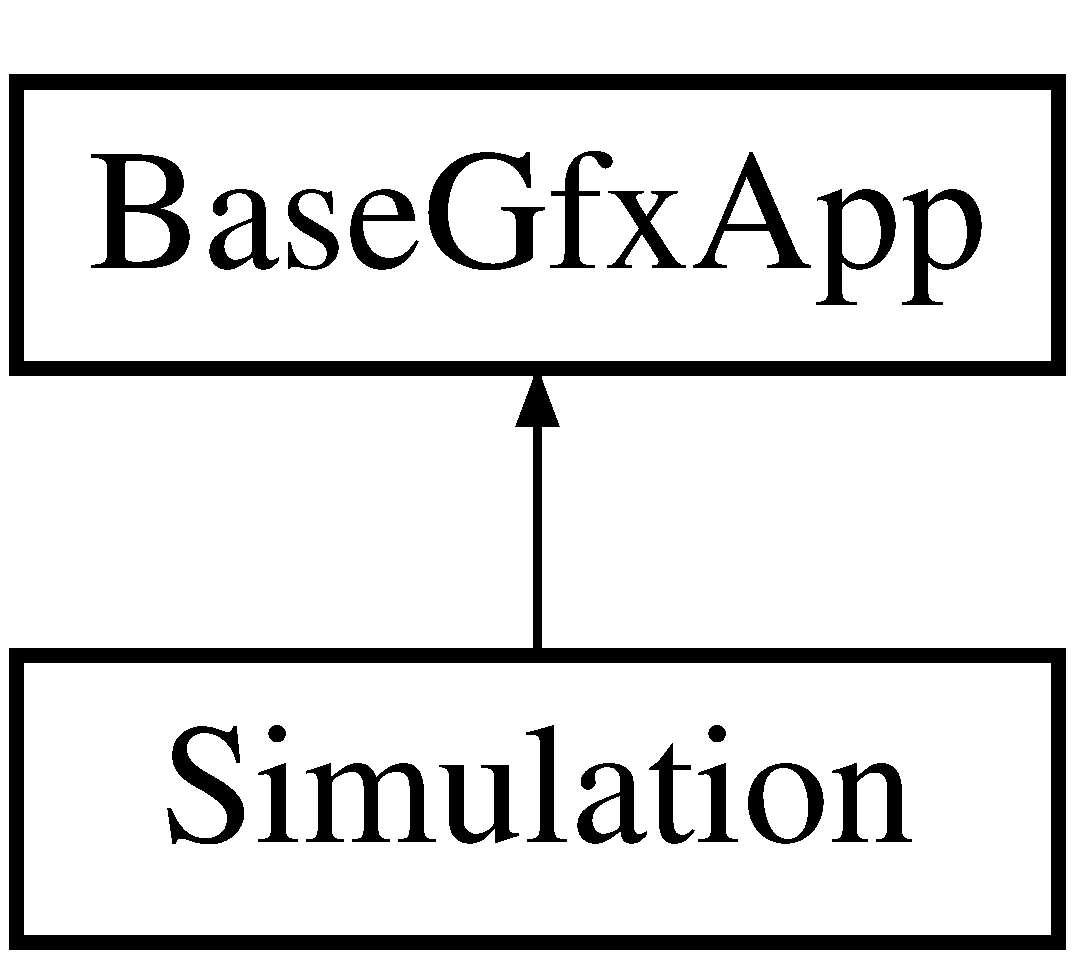
\includegraphics[height=2.000000cm]{classSimulation}
\end{center}
\end{figure}
\subsection*{Public Types}
\begin{DoxyCompactItemize}
\item 
enum \hyperlink{classSimulation_a0fd1c91d4e7699e893929d56b60a60bf}{U\-I\-Control\-Type} \{ \\*
\hyperlink{classSimulation_a0fd1c91d4e7699e893929d56b60a60bfa51f628c4a96a151830bd4a541dc42a5f}{U\-I\-\_\-\-Q\-U\-I\-T}, 
\hyperlink{classSimulation_a0fd1c91d4e7699e893929d56b60a60bfae8829fdccf0a3a28e0b0bf8dc47bf26e}{U\-I\-\_\-\-R\-E\-S\-U\-M\-E}, 
\hyperlink{classSimulation_a0fd1c91d4e7699e893929d56b60a60bfa6eb81d656b8ff64239548e4195560ef0}{U\-I\-\_\-\-P\-A\-U\-S\-E}, 
\hyperlink{classSimulation_a0fd1c91d4e7699e893929d56b60a60bfae4ec551adee29b6e2329929952c10ce5}{U\-I\-\_\-\-S\-T\-A\-R\-T}, 
\\*
\hyperlink{classSimulation_a0fd1c91d4e7699e893929d56b60a60bfa34512906ee0d0aafcd7f3257f738de15}{U\-I\-\_\-\-S\-P\-I\-N}
 \}
\begin{DoxyCompactList}\small\item\em the type of U\-I Control input. \end{DoxyCompactList}\end{DoxyCompactItemize}
\subsection*{Public Member Functions}
\begin{DoxyCompactItemize}
\item 
\hyperlink{classSimulation_a4c669ceaa34c7130966ce45f9de75fbe}{Simulation} (int argc, char $\ast$argv\mbox{[}$\,$\mbox{]}, int \hyperlink{classBaseGfxApp_ace089a1a94fb6bb0bc17e1b7fa48e05d}{width}, int \hyperlink{classBaseGfxApp_aa253dbe16a20c40e0a1bf8ff942ceea3}{height})
\begin{DoxyCompactList}\small\item\em arguements from user's command input and other window information. \end{DoxyCompactList}\item 
virtual \hyperlink{classSimulation_a80fad3f57dfaf195a36f7bc49bc88279}{$\sim$\-Simulation} ()
\item 
void \hyperlink{classSimulation_a449dcb7d97dfba99efe770de2f399c31}{display} ()
\begin{DoxyCompactList}\small\item\em display all the items. \end{DoxyCompactList}\item 
void \hyperlink{classSimulation_a1607cd18e552ab9f4a6f57d362f7121a}{glui\-Control} (int control\-I\-D)
\begin{DoxyCompactList}\small\item\em set controlflag value, in order to implement control panel. \end{DoxyCompactList}\item 
void \hyperlink{classSimulation_aa975d7962f1ea62a2c3a1ae42392d906}{render\-Robot} (\hyperlink{classRobotClass}{Robot\-Class} robot, int \hyperlink{classSimulation_a5a5e26d75c6a6dee8cdfecc7669545e3}{count})
\begin{DoxyCompactList}\small\item\em draw robot and send it to the window. \end{DoxyCompactList}\item 
void \hyperlink{classSimulation_a43ebad86548efc30eb3a3e9959002aaa}{render\-Light} (\hyperlink{classLight}{Light} light, int \hyperlink{classSimulation_a5a5e26d75c6a6dee8cdfecc7669545e3}{count})
\begin{DoxyCompactList}\small\item\em draw light and send it to the window. \end{DoxyCompactList}\item 
void \hyperlink{classSimulation_a786d1ba31d29937f0ac6f3ea88f8a607}{left\-Mouse\-Down} (int x, int y)
\begin{DoxyCompactList}\small\item\em The action will be taken when left mouse is clicked. \end{DoxyCompactList}\item 
void \hyperlink{classSimulation_a62ef254d85017074cd521a5787b5a234}{left\-Mouse\-Up} (int x, int y)
\begin{DoxyCompactList}\small\item\em The action will be taken when right mouse is clicked. \end{DoxyCompactList}\end{DoxyCompactItemize}
\subsection*{Private Attributes}
\begin{DoxyCompactItemize}
\item 
bool \hyperlink{classSimulation_a99785aef857b01f3056bada702b53d20}{controlflag}
\item 
int \hyperlink{classSimulation_aed3fe9fceae4a68746206b7a2f9e9d7f}{num\-Robot}
\item 
int \hyperlink{classSimulation_a792ef5172ff14046a641661ce2a95041}{num\-Light}
\item 
double \hyperlink{classSimulation_a9d5a2c76548907940c15b389344365df}{old\-Time\-Since\-Start}
\item 
vector$<$ \hyperlink{classRobotClass}{Robot\-Class} $>$ \hyperlink{classSimulation_ac48312060cc6b3b973bba8c802b45bce}{robots}
\item 
vector$<$ \hyperlink{classLight}{Light} $>$ \hyperlink{classSimulation_a4f6efa5f1bb16876c98f134fe80e9278}{lights}
\item 
\hyperlink{classEnvironmentClass}{Environment\-Class} $\ast$ \hyperlink{classSimulation_adb82ccf6c2a4b78c73987857f5362a35}{env}
\item 
G\-L\-U\-I\-\_\-\-Spinner $\ast$ \hyperlink{classSimulation_ade4b147d7d59002d1ea81b60bba84b48}{spinner}
\item 
int \hyperlink{classSimulation_a5a5e26d75c6a6dee8cdfecc7669545e3}{count}
\end{DoxyCompactItemize}
\subsection*{Additional Inherited Members}


\subsection{Detailed Description}
The \hyperlink{classSimulation}{Simulation} class. This sets up the G\-U\-I and the drawing environment. 

\subsection{Member Enumeration Documentation}
\hypertarget{classSimulation_a0fd1c91d4e7699e893929d56b60a60bf}{\index{Simulation@{Simulation}!U\-I\-Control\-Type@{U\-I\-Control\-Type}}
\index{U\-I\-Control\-Type@{U\-I\-Control\-Type}!Simulation@{Simulation}}
\subsubsection[{U\-I\-Control\-Type}]{\setlength{\rightskip}{0pt plus 5cm}enum {\bf Simulation\-::\-U\-I\-Control\-Type}}}\label{classSimulation_a0fd1c91d4e7699e893929d56b60a60bf}


the type of U\-I Control input. 

\begin{DoxyAuthor}{Author}
Zixiao Wang 
\end{DoxyAuthor}
\begin{Desc}
\item[Enumerator]\par
\begin{description}
\index{U\-I\-\_\-\-Q\-U\-I\-T@{U\-I\-\_\-\-Q\-U\-I\-T}!Simulation@{Simulation}}\index{Simulation@{Simulation}!U\-I\-\_\-\-Q\-U\-I\-T@{U\-I\-\_\-\-Q\-U\-I\-T}}\item[{\em 
\hypertarget{classSimulation_a0fd1c91d4e7699e893929d56b60a60bfa51f628c4a96a151830bd4a541dc42a5f}{U\-I\-\_\-\-Q\-U\-I\-T}\label{classSimulation_a0fd1c91d4e7699e893929d56b60a60bfa51f628c4a96a151830bd4a541dc42a5f}
}]\index{U\-I\-\_\-\-R\-E\-S\-U\-M\-E@{U\-I\-\_\-\-R\-E\-S\-U\-M\-E}!Simulation@{Simulation}}\index{Simulation@{Simulation}!U\-I\-\_\-\-R\-E\-S\-U\-M\-E@{U\-I\-\_\-\-R\-E\-S\-U\-M\-E}}\item[{\em 
\hypertarget{classSimulation_a0fd1c91d4e7699e893929d56b60a60bfae8829fdccf0a3a28e0b0bf8dc47bf26e}{U\-I\-\_\-\-R\-E\-S\-U\-M\-E}\label{classSimulation_a0fd1c91d4e7699e893929d56b60a60bfae8829fdccf0a3a28e0b0bf8dc47bf26e}
}]\index{U\-I\-\_\-\-P\-A\-U\-S\-E@{U\-I\-\_\-\-P\-A\-U\-S\-E}!Simulation@{Simulation}}\index{Simulation@{Simulation}!U\-I\-\_\-\-P\-A\-U\-S\-E@{U\-I\-\_\-\-P\-A\-U\-S\-E}}\item[{\em 
\hypertarget{classSimulation_a0fd1c91d4e7699e893929d56b60a60bfa6eb81d656b8ff64239548e4195560ef0}{U\-I\-\_\-\-P\-A\-U\-S\-E}\label{classSimulation_a0fd1c91d4e7699e893929d56b60a60bfa6eb81d656b8ff64239548e4195560ef0}
}]\index{U\-I\-\_\-\-S\-T\-A\-R\-T@{U\-I\-\_\-\-S\-T\-A\-R\-T}!Simulation@{Simulation}}\index{Simulation@{Simulation}!U\-I\-\_\-\-S\-T\-A\-R\-T@{U\-I\-\_\-\-S\-T\-A\-R\-T}}\item[{\em 
\hypertarget{classSimulation_a0fd1c91d4e7699e893929d56b60a60bfae4ec551adee29b6e2329929952c10ce5}{U\-I\-\_\-\-S\-T\-A\-R\-T}\label{classSimulation_a0fd1c91d4e7699e893929d56b60a60bfae4ec551adee29b6e2329929952c10ce5}
}]\index{U\-I\-\_\-\-S\-P\-I\-N@{U\-I\-\_\-\-S\-P\-I\-N}!Simulation@{Simulation}}\index{Simulation@{Simulation}!U\-I\-\_\-\-S\-P\-I\-N@{U\-I\-\_\-\-S\-P\-I\-N}}\item[{\em 
\hypertarget{classSimulation_a0fd1c91d4e7699e893929d56b60a60bfa34512906ee0d0aafcd7f3257f738de15}{U\-I\-\_\-\-S\-P\-I\-N}\label{classSimulation_a0fd1c91d4e7699e893929d56b60a60bfa34512906ee0d0aafcd7f3257f738de15}
}]\end{description}
\end{Desc}


\subsection{Constructor \& Destructor Documentation}
\hypertarget{classSimulation_a4c669ceaa34c7130966ce45f9de75fbe}{\index{Simulation@{Simulation}!Simulation@{Simulation}}
\index{Simulation@{Simulation}!Simulation@{Simulation}}
\subsubsection[{Simulation}]{\setlength{\rightskip}{0pt plus 5cm}Simulation\-::\-Simulation (
\begin{DoxyParamCaption}
\item[{int}]{argc, }
\item[{char $\ast$}]{argv\mbox{[}$\,$\mbox{]}, }
\item[{int}]{width, }
\item[{int}]{height}
\end{DoxyParamCaption}
)}}\label{classSimulation_a4c669ceaa34c7130966ce45f9de75fbe}


arguements from user's command input and other window information. 

\begin{DoxyAuthor}{Author}
Zixiao Wang 
\end{DoxyAuthor}

\begin{DoxyParams}{Parameters}
{\em argc} & The number of command arguement. \\
\hline
{\em argv} & The command input array. \\
\hline
{\em width} & The width of window. \\
\hline
{\em height} & The height of window. \\
\hline
\end{DoxyParams}
\hypertarget{classSimulation_a80fad3f57dfaf195a36f7bc49bc88279}{\index{Simulation@{Simulation}!$\sim$\-Simulation@{$\sim$\-Simulation}}
\index{$\sim$\-Simulation@{$\sim$\-Simulation}!Simulation@{Simulation}}
\subsubsection[{$\sim$\-Simulation}]{\setlength{\rightskip}{0pt plus 5cm}Simulation\-::$\sim$\-Simulation (
\begin{DoxyParamCaption}
{}
\end{DoxyParamCaption}
)\hspace{0.3cm}{\ttfamily [virtual]}}}\label{classSimulation_a80fad3f57dfaf195a36f7bc49bc88279}


\subsection{Member Function Documentation}
\hypertarget{classSimulation_a449dcb7d97dfba99efe770de2f399c31}{\index{Simulation@{Simulation}!display@{display}}
\index{display@{display}!Simulation@{Simulation}}
\subsubsection[{display}]{\setlength{\rightskip}{0pt plus 5cm}void Simulation\-::display (
\begin{DoxyParamCaption}
{}
\end{DoxyParamCaption}
)\hspace{0.3cm}{\ttfamily [virtual]}}}\label{classSimulation_a449dcb7d97dfba99efe770de2f399c31}


display all the items. 

\begin{DoxyAuthor}{Author}
Zixiao Wang and Triny Chen 
\end{DoxyAuthor}


Reimplemented from \hyperlink{classBaseGfxApp_ac8de2d5a955582547af5619b771b4d6d}{Base\-Gfx\-App}.

\hypertarget{classSimulation_a1607cd18e552ab9f4a6f57d362f7121a}{\index{Simulation@{Simulation}!glui\-Control@{glui\-Control}}
\index{glui\-Control@{glui\-Control}!Simulation@{Simulation}}
\subsubsection[{glui\-Control}]{\setlength{\rightskip}{0pt plus 5cm}void Simulation\-::glui\-Control (
\begin{DoxyParamCaption}
\item[{int}]{control\-I\-D}
\end{DoxyParamCaption}
)\hspace{0.3cm}{\ttfamily [virtual]}}}\label{classSimulation_a1607cd18e552ab9f4a6f57d362f7121a}


set controlflag value, in order to implement control panel. 

\begin{DoxyAuthor}{Author}
Zixiao Wang 
\end{DoxyAuthor}


Reimplemented from \hyperlink{classBaseGfxApp_a2978a7c358794c67df73b66776b2cef3}{Base\-Gfx\-App}.

\hypertarget{classSimulation_a786d1ba31d29937f0ac6f3ea88f8a607}{\index{Simulation@{Simulation}!left\-Mouse\-Down@{left\-Mouse\-Down}}
\index{left\-Mouse\-Down@{left\-Mouse\-Down}!Simulation@{Simulation}}
\subsubsection[{left\-Mouse\-Down}]{\setlength{\rightskip}{0pt plus 5cm}void Simulation\-::left\-Mouse\-Down (
\begin{DoxyParamCaption}
\item[{int}]{x, }
\item[{int}]{y}
\end{DoxyParamCaption}
)\hspace{0.3cm}{\ttfamily [virtual]}}}\label{classSimulation_a786d1ba31d29937f0ac6f3ea88f8a607}


The action will be taken when left mouse is clicked. 


\begin{DoxyParams}{Parameters}
{\em x} & the x position of mouse click position. \\
\hline
{\em y} & the y position of mouse click position. \\
\hline
\end{DoxyParams}


Reimplemented from \hyperlink{classBaseGfxApp_aaaccf5a5e923a9465441a5ee712424a8}{Base\-Gfx\-App}.

\hypertarget{classSimulation_a62ef254d85017074cd521a5787b5a234}{\index{Simulation@{Simulation}!left\-Mouse\-Up@{left\-Mouse\-Up}}
\index{left\-Mouse\-Up@{left\-Mouse\-Up}!Simulation@{Simulation}}
\subsubsection[{left\-Mouse\-Up}]{\setlength{\rightskip}{0pt plus 5cm}void Simulation\-::left\-Mouse\-Up (
\begin{DoxyParamCaption}
\item[{int}]{x, }
\item[{int}]{y}
\end{DoxyParamCaption}
)\hspace{0.3cm}{\ttfamily [virtual]}}}\label{classSimulation_a62ef254d85017074cd521a5787b5a234}


The action will be taken when right mouse is clicked. 


\begin{DoxyParams}{Parameters}
{\em x} & the x position of mouse click position. \\
\hline
{\em y} & the y position of mouse click position. \\
\hline
\end{DoxyParams}


Reimplemented from \hyperlink{classBaseGfxApp_a0a2961a932b02b2f9d7d0bb408f6fb51}{Base\-Gfx\-App}.

\hypertarget{classSimulation_a43ebad86548efc30eb3a3e9959002aaa}{\index{Simulation@{Simulation}!render\-Light@{render\-Light}}
\index{render\-Light@{render\-Light}!Simulation@{Simulation}}
\subsubsection[{render\-Light}]{\setlength{\rightskip}{0pt plus 5cm}void Simulation\-::render\-Light (
\begin{DoxyParamCaption}
\item[{{\bf Light}}]{light, }
\item[{int}]{count}
\end{DoxyParamCaption}
)}}\label{classSimulation_a43ebad86548efc30eb3a3e9959002aaa}


draw light and send it to the window. 

\begin{DoxyAuthor}{Author}
Zixiao Wang 
\end{DoxyAuthor}

\begin{DoxyParams}{Parameters}
{\em light} & pass in the light which is to be sent. \\
\hline
{\em count} & used for changing color \\
\hline
\end{DoxyParams}
\hypertarget{classSimulation_aa975d7962f1ea62a2c3a1ae42392d906}{\index{Simulation@{Simulation}!render\-Robot@{render\-Robot}}
\index{render\-Robot@{render\-Robot}!Simulation@{Simulation}}
\subsubsection[{render\-Robot}]{\setlength{\rightskip}{0pt plus 5cm}void Simulation\-::render\-Robot (
\begin{DoxyParamCaption}
\item[{{\bf Robot\-Class}}]{robot, }
\item[{int}]{count}
\end{DoxyParamCaption}
)}}\label{classSimulation_aa975d7962f1ea62a2c3a1ae42392d906}


draw robot and send it to the window. 

\begin{DoxyAuthor}{Author}
Zixiao Wang 
\end{DoxyAuthor}

\begin{DoxyParams}{Parameters}
{\em robot} & pass in the robot which is to be sent. \\
\hline
{\em count} & used for changing color \\
\hline
\end{DoxyParams}


\subsection{Member Data Documentation}
\hypertarget{classSimulation_a99785aef857b01f3056bada702b53d20}{\index{Simulation@{Simulation}!controlflag@{controlflag}}
\index{controlflag@{controlflag}!Simulation@{Simulation}}
\subsubsection[{controlflag}]{\setlength{\rightskip}{0pt plus 5cm}bool Simulation\-::controlflag\hspace{0.3cm}{\ttfamily [private]}}}\label{classSimulation_a99785aef857b01f3056bada702b53d20}
The flag for panel input \hypertarget{classSimulation_a5a5e26d75c6a6dee8cdfecc7669545e3}{\index{Simulation@{Simulation}!count@{count}}
\index{count@{count}!Simulation@{Simulation}}
\subsubsection[{count}]{\setlength{\rightskip}{0pt plus 5cm}int Simulation\-::count\hspace{0.3cm}{\ttfamily [private]}}}\label{classSimulation_a5a5e26d75c6a6dee8cdfecc7669545e3}
\hypertarget{classSimulation_adb82ccf6c2a4b78c73987857f5362a35}{\index{Simulation@{Simulation}!env@{env}}
\index{env@{env}!Simulation@{Simulation}}
\subsubsection[{env}]{\setlength{\rightskip}{0pt plus 5cm}{\bf Environment\-Class}$\ast$ Simulation\-::env\hspace{0.3cm}{\ttfamily [private]}}}\label{classSimulation_adb82ccf6c2a4b78c73987857f5362a35}
A environment created \hypertarget{classSimulation_a4f6efa5f1bb16876c98f134fe80e9278}{\index{Simulation@{Simulation}!lights@{lights}}
\index{lights@{lights}!Simulation@{Simulation}}
\subsubsection[{lights}]{\setlength{\rightskip}{0pt plus 5cm}vector$<${\bf Light}$>$ Simulation\-::lights\hspace{0.3cm}{\ttfamily [private]}}}\label{classSimulation_a4f6efa5f1bb16876c98f134fe80e9278}
A vector of lights created \hypertarget{classSimulation_a792ef5172ff14046a641661ce2a95041}{\index{Simulation@{Simulation}!num\-Light@{num\-Light}}
\index{num\-Light@{num\-Light}!Simulation@{Simulation}}
\subsubsection[{num\-Light}]{\setlength{\rightskip}{0pt plus 5cm}int Simulation\-::num\-Light\hspace{0.3cm}{\ttfamily [private]}}}\label{classSimulation_a792ef5172ff14046a641661ce2a95041}
The number of target \hypertarget{classSimulation_aed3fe9fceae4a68746206b7a2f9e9d7f}{\index{Simulation@{Simulation}!num\-Robot@{num\-Robot}}
\index{num\-Robot@{num\-Robot}!Simulation@{Simulation}}
\subsubsection[{num\-Robot}]{\setlength{\rightskip}{0pt plus 5cm}int Simulation\-::num\-Robot\hspace{0.3cm}{\ttfamily [private]}}}\label{classSimulation_aed3fe9fceae4a68746206b7a2f9e9d7f}
The number of robot \hypertarget{classSimulation_a9d5a2c76548907940c15b389344365df}{\index{Simulation@{Simulation}!old\-Time\-Since\-Start@{old\-Time\-Since\-Start}}
\index{old\-Time\-Since\-Start@{old\-Time\-Since\-Start}!Simulation@{Simulation}}
\subsubsection[{old\-Time\-Since\-Start}]{\setlength{\rightskip}{0pt plus 5cm}double Simulation\-::old\-Time\-Since\-Start\hspace{0.3cm}{\ttfamily [private]}}}\label{classSimulation_a9d5a2c76548907940c15b389344365df}
The time since the start \hypertarget{classSimulation_ac48312060cc6b3b973bba8c802b45bce}{\index{Simulation@{Simulation}!robots@{robots}}
\index{robots@{robots}!Simulation@{Simulation}}
\subsubsection[{robots}]{\setlength{\rightskip}{0pt plus 5cm}vector$<${\bf Robot\-Class}$>$ Simulation\-::robots\hspace{0.3cm}{\ttfamily [private]}}}\label{classSimulation_ac48312060cc6b3b973bba8c802b45bce}
A vector of robots created \hypertarget{classSimulation_ade4b147d7d59002d1ea81b60bba84b48}{\index{Simulation@{Simulation}!spinner@{spinner}}
\index{spinner@{spinner}!Simulation@{Simulation}}
\subsubsection[{spinner}]{\setlength{\rightskip}{0pt plus 5cm}G\-L\-U\-I\-\_\-\-Spinner$\ast$ Simulation\-::spinner\hspace{0.3cm}{\ttfamily [private]}}}\label{classSimulation_ade4b147d7d59002d1ea81b60bba84b48}
A panel spinner 

The documentation for this class was generated from the following files\-:\begin{DoxyCompactItemize}
\item 
\hyperlink{Simulation_8h}{Simulation.\-h}\item 
\hyperlink{Simulation_8cpp}{Simulation.\-cpp}\end{DoxyCompactItemize}

\chapter{File Documentation}
\hypertarget{BaseGfxApp_8cpp}{\section{Base\-Gfx\-App.\-cpp File Reference}
\label{BaseGfxApp_8cpp}\index{Base\-Gfx\-App.\-cpp@{Base\-Gfx\-App.\-cpp}}
}
{\ttfamily \#include \char`\"{}Base\-Gfx\-App.\-h\char`\"{}}\\*
\subsection*{Macros}
\begin{DoxyCompactItemize}
\item 
\#define \hyperlink{BaseGfxApp_8cpp_a38533d3b08eadb4b2e6fe2f443dd83f1}{I\-N\-I\-T\-\_\-\-W\-I\-D\-T\-H}~800
\item 
\#define \hyperlink{BaseGfxApp_8cpp_acd7e35d0c6cca5b5b665b77b5377c4a0}{I\-N\-I\-T\-\_\-\-H\-E\-I\-G\-H\-T}~600
\end{DoxyCompactItemize}


\subsection{Macro Definition Documentation}
\hypertarget{BaseGfxApp_8cpp_acd7e35d0c6cca5b5b665b77b5377c4a0}{\index{Base\-Gfx\-App.\-cpp@{Base\-Gfx\-App.\-cpp}!I\-N\-I\-T\-\_\-\-H\-E\-I\-G\-H\-T@{I\-N\-I\-T\-\_\-\-H\-E\-I\-G\-H\-T}}
\index{I\-N\-I\-T\-\_\-\-H\-E\-I\-G\-H\-T@{I\-N\-I\-T\-\_\-\-H\-E\-I\-G\-H\-T}!BaseGfxApp.cpp@{Base\-Gfx\-App.\-cpp}}
\subsubsection[{I\-N\-I\-T\-\_\-\-H\-E\-I\-G\-H\-T}]{\setlength{\rightskip}{0pt plus 5cm}\#define I\-N\-I\-T\-\_\-\-H\-E\-I\-G\-H\-T~600}}\label{BaseGfxApp_8cpp_acd7e35d0c6cca5b5b665b77b5377c4a0}
\hypertarget{BaseGfxApp_8cpp_a38533d3b08eadb4b2e6fe2f443dd83f1}{\index{Base\-Gfx\-App.\-cpp@{Base\-Gfx\-App.\-cpp}!I\-N\-I\-T\-\_\-\-W\-I\-D\-T\-H@{I\-N\-I\-T\-\_\-\-W\-I\-D\-T\-H}}
\index{I\-N\-I\-T\-\_\-\-W\-I\-D\-T\-H@{I\-N\-I\-T\-\_\-\-W\-I\-D\-T\-H}!BaseGfxApp.cpp@{Base\-Gfx\-App.\-cpp}}
\subsubsection[{I\-N\-I\-T\-\_\-\-W\-I\-D\-T\-H}]{\setlength{\rightskip}{0pt plus 5cm}\#define I\-N\-I\-T\-\_\-\-W\-I\-D\-T\-H~800}}\label{BaseGfxApp_8cpp_a38533d3b08eadb4b2e6fe2f443dd83f1}

\hypertarget{BaseGfxApp_8h}{\section{Base\-Gfx\-App.\-h File Reference}
\label{BaseGfxApp_8h}\index{Base\-Gfx\-App.\-h@{Base\-Gfx\-App.\-h}}
}


The basic application class for C\-Sci-\/3081 project. Uses G\-L\-U\-T and G\-L\-U\-I and wraps them in a nice C++ interface.  


{\ttfamily \#include $<$string$>$}\\*
{\ttfamily \#include $<$iostream$>$}\\*
{\ttfamily \#include $<$assert.\-h$>$}\\*
{\ttfamily \#include $<$G\-L/glui.\-h$>$}\\*
\subsection*{Classes}
\begin{DoxyCompactItemize}
\item 
class \hyperlink{classBaseGfxApp}{Base\-Gfx\-App}
\end{DoxyCompactItemize}


\subsection{Detailed Description}
The basic application class for C\-Sci-\/3081 project. Uses G\-L\-U\-T and G\-L\-U\-I and wraps them in a nice C++ interface. \begin{DoxyAuthor}{Author}
C\-Sci3081 Guru 
\end{DoxyAuthor}

\hypertarget{EnvironmentClass_8cpp}{\section{Environment\-Class.\-cpp File Reference}
\label{EnvironmentClass_8cpp}\index{Environment\-Class.\-cpp@{Environment\-Class.\-cpp}}
}
{\ttfamily \#include \char`\"{}Environment\-Class.\-h\char`\"{}}\\*
{\ttfamily \#include $<$math.\-h$>$}\\*
{\ttfamily \#include $<$G\-L/glut.\-h$>$}\\*
{\ttfamily \#include $<$stdlib.\-h$>$}\\*

\hypertarget{EnvironmentClass_8h}{\section{Environment\-Class.\-h File Reference}
\label{EnvironmentClass_8h}\index{Environment\-Class.\-h@{Environment\-Class.\-h}}
}


Main application class for the Environment Class.  


{\ttfamily \#include \char`\"{}Robot\-Class.\-h\char`\"{}}\\*
{\ttfamily \#include \char`\"{}Light.\-h\char`\"{}}\\*
{\ttfamily \#include $<$vector$>$}\\*
{\ttfamily \#include $<$iostream$>$}\\*
\subsection*{Classes}
\begin{DoxyCompactItemize}
\item 
class \hyperlink{classEnvironmentClass}{Environment\-Class}
\end{DoxyCompactItemize}


\subsection{Detailed Description}
Main application class for the Environment Class. \begin{DoxyAuthor}{Author}
Group Meryl\-\_\-\-Streep 
\end{DoxyAuthor}
\begin{DoxyDate}{Date}
10 April 2015 
\end{DoxyDate}

\hypertarget{EnvironmentClassTest_8h}{\section{Environment\-Class\-Test.\-h File Reference}
\label{EnvironmentClassTest_8h}\index{Environment\-Class\-Test.\-h@{Environment\-Class\-Test.\-h}}
}


The Tests for environment functions.  


{\ttfamily \#include $<$cxxtest/\-Test\-Suite.\-h$>$}\\*
{\ttfamily \#include \char`\"{}Environment\-Class.\-h\char`\"{}}\\*
{\ttfamily \#include $<$math.\-h$>$}\\*
{\ttfamily \#include $<$G\-L/glut.\-h$>$}\\*
{\ttfamily \#include \char`\"{}Object.\-h\char`\"{}}\\*
{\ttfamily \#include $<$stdlib.\-h$>$}\\*
\subsection*{Classes}
\begin{DoxyCompactItemize}
\item 
class \hyperlink{classEnvironmentClassTest}{Environment\-Class\-Test}
\end{DoxyCompactItemize}


\subsection{Detailed Description}
The Tests for environment functions. \begin{DoxyAuthor}{Author}
Group Meryl\-\_\-\-Streep 
\end{DoxyAuthor}
\begin{DoxyDate}{Date}
12 Mar 2015 
\end{DoxyDate}

\hypertarget{main_8cpp}{\section{main.\-cpp File Reference}
\label{main_8cpp}\index{main.\-cpp@{main.\-cpp}}
}


Main function.  


{\ttfamily \#include \char`\"{}Simulation.\-h\char`\"{}}\\*
\subsection*{Functions}
\begin{DoxyCompactItemize}
\item 
int \hyperlink{main_8cpp_a0ddf1224851353fc92bfbff6f499fa97}{main} (int argc, char $\ast$argv\mbox{[}$\,$\mbox{]})
\end{DoxyCompactItemize}


\subsection{Detailed Description}
Main function. \begin{DoxyAuthor}{Author}
C\-Sci5107 Guru 
\end{DoxyAuthor}


\subsection{Function Documentation}
\hypertarget{main_8cpp_a0ddf1224851353fc92bfbff6f499fa97}{\index{main.\-cpp@{main.\-cpp}!main@{main}}
\index{main@{main}!main.cpp@{main.\-cpp}}
\subsubsection[{main}]{\setlength{\rightskip}{0pt plus 5cm}int main (
\begin{DoxyParamCaption}
\item[{int}]{argc, }
\item[{char $\ast$}]{argv\mbox{[}$\,$\mbox{]}}
\end{DoxyParamCaption}
)}}\label{main_8cpp_a0ddf1224851353fc92bfbff6f499fa97}

\hypertarget{Object_8cpp}{\section{Object.\-cpp File Reference}
\label{Object_8cpp}\index{Object.\-cpp@{Object.\-cpp}}
}


The representation of \hyperlink{classObject}{Object} within the simulation.  


{\ttfamily \#include \char`\"{}Object.\-h\char`\"{}}\\*
{\ttfamily \#include $<$iostream$>$}\\*


\subsection{Detailed Description}
The representation of \hyperlink{classObject}{Object} within the simulation. \begin{DoxyAuthor}{Author}
Group Meryl\-\_\-\-Streep 
\end{DoxyAuthor}
\begin{DoxyDate}{Date}
9 March 2015 
\end{DoxyDate}

\hypertarget{Object_8h}{\section{Object.\-h File Reference}
\label{Object_8h}\index{Object.\-h@{Object.\-h}}
}


The \hyperlink{classObject}{Object} Class.  


{\ttfamily \#include $<$stdlib.\-h$>$}\\*
\subsection*{Classes}
\begin{DoxyCompactItemize}
\item 
struct \hyperlink{structNavigate}{Navigate}
\item 
class \hyperlink{classObject}{Object}
\begin{DoxyCompactList}\small\item\em Super Class of Robot\-Class, Target and Obstacle, contains position x, y and size. \end{DoxyCompactList}\end{DoxyCompactItemize}
\subsection*{Enumerations}
\begin{DoxyCompactItemize}
\item 
enum \hyperlink{Object_8h_a842c5e2e69277690b064bf363c017980}{Object\-Type} \{ \hyperlink{Object_8h_a842c5e2e69277690b064bf363c017980a0349261f505b36305e1a7468fd941de8}{Robot}, 
\hyperlink{Object_8h_a842c5e2e69277690b064bf363c017980a297b29d409921385e20239f12db235ed}{Obstacle}, 
\hyperlink{Object_8h_a842c5e2e69277690b064bf363c017980a444cbec7ad70f50f8eec3f6fa116d1da}{Target}
 \}
\item 
enum \hyperlink{Object_8h_a5a4538eeab397888d88a4eefcc5a1345}{Shape\-Type} \{ \hyperlink{Object_8h_a5a4538eeab397888d88a4eefcc5a1345ad3ce82743a8255ccd69f5b67d257c489}{Circle}, 
\hyperlink{Object_8h_a5a4538eeab397888d88a4eefcc5a1345a773e9be14af3bc697c412f3e6c5c509e}{Triangle}, 
\hyperlink{Object_8h_a5a4538eeab397888d88a4eefcc5a1345a349990a9494411f297f9349ed29172b3}{Quad}
 \}
\item 
enum \hyperlink{Object_8h_ad4f6886266572e51d198a61a6c762ce5}{Wall} \{ \\*
\hyperlink{Object_8h_ad4f6886266572e51d198a61a6c762ce5ac9d3e887722f2bc482bcca9d41c512af}{None}, 
\hyperlink{Object_8h_ad4f6886266572e51d198a61a6c762ce5a47321105d20c4efd6c573a6d829e1ad9}{Top}, 
\hyperlink{Object_8h_ad4f6886266572e51d198a61a6c762ce5a05cdd4fa6b505ee008f4e865acfecccb}{Bottom}, 
\hyperlink{Object_8h_ad4f6886266572e51d198a61a6c762ce5a9d4d8b0b72fc2659da772d761a3c5ecb}{Left}, 
\\*
\hyperlink{Object_8h_ad4f6886266572e51d198a61a6c762ce5ad48f7af8c070184f3774c8e85854eb66}{Right}
 \}
\end{DoxyCompactItemize}


\subsection{Detailed Description}
The \hyperlink{classObject}{Object} Class. \begin{DoxyAuthor}{Author}
Group Meryl\-\_\-\-Streep 
\end{DoxyAuthor}
\begin{DoxyDate}{Date}
9 March 2015 
\end{DoxyDate}


\subsection{Enumeration Type Documentation}
\hypertarget{Object_8h_a842c5e2e69277690b064bf363c017980}{\index{Object.\-h@{Object.\-h}!Object\-Type@{Object\-Type}}
\index{Object\-Type@{Object\-Type}!Object.h@{Object.\-h}}
\subsubsection[{Object\-Type}]{\setlength{\rightskip}{0pt plus 5cm}enum {\bf Object\-Type}}}\label{Object_8h_a842c5e2e69277690b064bf363c017980}
\begin{Desc}
\item[Enumerator]\par
\begin{description}
\index{Robot@{Robot}!Object.\-h@{Object.\-h}}\index{Object.\-h@{Object.\-h}!Robot@{Robot}}\item[{\em 
\hypertarget{Object_8h_a842c5e2e69277690b064bf363c017980a0349261f505b36305e1a7468fd941de8}{Robot}\label{Object_8h_a842c5e2e69277690b064bf363c017980a0349261f505b36305e1a7468fd941de8}
}]Type of \hyperlink{classObject}{Object} \index{Obstacle@{Obstacle}!Object.\-h@{Object.\-h}}\index{Object.\-h@{Object.\-h}!Obstacle@{Obstacle}}\item[{\em 
\hypertarget{Object_8h_a842c5e2e69277690b064bf363c017980a297b29d409921385e20239f12db235ed}{Obstacle}\label{Object_8h_a842c5e2e69277690b064bf363c017980a297b29d409921385e20239f12db235ed}
}]\index{Target@{Target}!Object.\-h@{Object.\-h}}\index{Object.\-h@{Object.\-h}!Target@{Target}}\item[{\em 
\hypertarget{Object_8h_a842c5e2e69277690b064bf363c017980a444cbec7ad70f50f8eec3f6fa116d1da}{Target}\label{Object_8h_a842c5e2e69277690b064bf363c017980a444cbec7ad70f50f8eec3f6fa116d1da}
}]\end{description}
\end{Desc}
\hypertarget{Object_8h_a5a4538eeab397888d88a4eefcc5a1345}{\index{Object.\-h@{Object.\-h}!Shape\-Type@{Shape\-Type}}
\index{Shape\-Type@{Shape\-Type}!Object.h@{Object.\-h}}
\subsubsection[{Shape\-Type}]{\setlength{\rightskip}{0pt plus 5cm}enum {\bf Shape\-Type}}}\label{Object_8h_a5a4538eeab397888d88a4eefcc5a1345}
\begin{Desc}
\item[Enumerator]\par
\begin{description}
\index{Circle@{Circle}!Object.\-h@{Object.\-h}}\index{Object.\-h@{Object.\-h}!Circle@{Circle}}\item[{\em 
\hypertarget{Object_8h_a5a4538eeab397888d88a4eefcc5a1345ad3ce82743a8255ccd69f5b67d257c489}{Circle}\label{Object_8h_a5a4538eeab397888d88a4eefcc5a1345ad3ce82743a8255ccd69f5b67d257c489}
}]Shape type of \hyperlink{classObject}{Object} \index{Triangle@{Triangle}!Object.\-h@{Object.\-h}}\index{Object.\-h@{Object.\-h}!Triangle@{Triangle}}\item[{\em 
\hypertarget{Object_8h_a5a4538eeab397888d88a4eefcc5a1345a773e9be14af3bc697c412f3e6c5c509e}{Triangle}\label{Object_8h_a5a4538eeab397888d88a4eefcc5a1345a773e9be14af3bc697c412f3e6c5c509e}
}]\index{Quad@{Quad}!Object.\-h@{Object.\-h}}\index{Object.\-h@{Object.\-h}!Quad@{Quad}}\item[{\em 
\hypertarget{Object_8h_a5a4538eeab397888d88a4eefcc5a1345a349990a9494411f297f9349ed29172b3}{Quad}\label{Object_8h_a5a4538eeab397888d88a4eefcc5a1345a349990a9494411f297f9349ed29172b3}
}]\end{description}
\end{Desc}
\hypertarget{Object_8h_ad4f6886266572e51d198a61a6c762ce5}{\index{Object.\-h@{Object.\-h}!Wall@{Wall}}
\index{Wall@{Wall}!Object.h@{Object.\-h}}
\subsubsection[{Wall}]{\setlength{\rightskip}{0pt plus 5cm}enum {\bf Wall}}}\label{Object_8h_ad4f6886266572e51d198a61a6c762ce5}
\begin{Desc}
\item[Enumerator]\par
\begin{description}
\index{None@{None}!Object.\-h@{Object.\-h}}\index{Object.\-h@{Object.\-h}!None@{None}}\item[{\em 
\hypertarget{Object_8h_ad4f6886266572e51d198a61a6c762ce5ac9d3e887722f2bc482bcca9d41c512af}{None}\label{Object_8h_ad4f6886266572e51d198a61a6c762ce5ac9d3e887722f2bc482bcca9d41c512af}
}]Different walls \index{Top@{Top}!Object.\-h@{Object.\-h}}\index{Object.\-h@{Object.\-h}!Top@{Top}}\item[{\em 
\hypertarget{Object_8h_ad4f6886266572e51d198a61a6c762ce5a47321105d20c4efd6c573a6d829e1ad9}{Top}\label{Object_8h_ad4f6886266572e51d198a61a6c762ce5a47321105d20c4efd6c573a6d829e1ad9}
}]\index{Bottom@{Bottom}!Object.\-h@{Object.\-h}}\index{Object.\-h@{Object.\-h}!Bottom@{Bottom}}\item[{\em 
\hypertarget{Object_8h_ad4f6886266572e51d198a61a6c762ce5a05cdd4fa6b505ee008f4e865acfecccb}{Bottom}\label{Object_8h_ad4f6886266572e51d198a61a6c762ce5a05cdd4fa6b505ee008f4e865acfecccb}
}]\index{Left@{Left}!Object.\-h@{Object.\-h}}\index{Object.\-h@{Object.\-h}!Left@{Left}}\item[{\em 
\hypertarget{Object_8h_ad4f6886266572e51d198a61a6c762ce5a9d4d8b0b72fc2659da772d761a3c5ecb}{Left}\label{Object_8h_ad4f6886266572e51d198a61a6c762ce5a9d4d8b0b72fc2659da772d761a3c5ecb}
}]\index{Right@{Right}!Object.\-h@{Object.\-h}}\index{Object.\-h@{Object.\-h}!Right@{Right}}\item[{\em 
\hypertarget{Object_8h_ad4f6886266572e51d198a61a6c762ce5ad48f7af8c070184f3774c8e85854eb66}{Right}\label{Object_8h_ad4f6886266572e51d198a61a6c762ce5ad48f7af8c070184f3774c8e85854eb66}
}]\end{description}
\end{Desc}

\hypertarget{ObjectTests_8h}{\section{Object\-Tests.\-h File Reference}
\label{ObjectTests_8h}\index{Object\-Tests.\-h@{Object\-Tests.\-h}}
}
{\ttfamily \#include \char`\"{}Object.\-h\char`\"{}}\\*
{\ttfamily \#include $<$iostream$>$}\\*
{\ttfamily \#include $<$cxxtest/\-Test\-Suite.\-h$>$}\\*
\subsection*{Classes}
\begin{DoxyCompactItemize}
\item 
class \hyperlink{classObjectTests}{Object\-Tests}
\end{DoxyCompactItemize}

\hypertarget{Simulation_8cpp}{\section{Simulation.\-cpp File Reference}
\label{Simulation_8cpp}\index{Simulation.\-cpp@{Simulation.\-cpp}}
}
{\ttfamily \#include \char`\"{}Simulation.\-h\char`\"{}}\\*
{\ttfamily \#include $<$math.\-h$>$}\\*
{\ttfamily \#include $<$time.\-h$>$}\\*

\hypertarget{Simulation_8h}{\section{Simulation.\-h File Reference}
\label{Simulation_8h}\index{Simulation.\-h@{Simulation.\-h}}
}


Main application class for the robot simulation.  


{\ttfamily \#include $<$vector$>$}\\*
{\ttfamily \#include $<$cstdlib$>$}\\*
{\ttfamily \#include \char`\"{}Base\-Gfx\-App.\-h\char`\"{}}\\*
{\ttfamily \#include \char`\"{}Environment\-Class.\-h\char`\"{}}\\*
{\ttfamily \#include \char`\"{}Object.\-h\char`\"{}}\\*
\subsection*{Classes}
\begin{DoxyCompactItemize}
\item 
class \hyperlink{classSimulation}{Simulation}
\end{DoxyCompactItemize}


\subsection{Detailed Description}
Main application class for the robot simulation. \begin{DoxyAuthor}{Author}
C\-Sci3081 Guru 
\end{DoxyAuthor}

%--- End generated contents ---

% Index
\newpage
\phantomsection
\addcontentsline{toc}{chapter}{Index}
\printindex

\end{document}
